%% An Introduction to LaTeX Thesis Template of Wuhan University
%%
%% Created by WHUTUG

\documentclass[type=master, class=professional]{whu-thesis}
\usepackage{rotating}
\usepackage{multirow}
\usepackage{graphicx}
\usepackage[normalem]{ulem}
\usepackage{booktabs}
% \usepackage[table,xcdraw]{xcolor}
\useunder{\uline}{\ul}{}
% 注释掉下面这行编译出来的即为插入空白页,不注释则为不插入空白页
\renewcommand{\cleardoublepage}{\clearpage}
\newcommand{\figcite}[1]{\scalebox{1.3}[1.3]{\raisebox{-0.7ex}{\cite{#1}}}}
\whusetup
  {
    info               =
      {
        title          = {跨域知识图谱的知识\\表示学习研究},
        title*         = {A Research on Knowledge Representation \\Learning in Cross-domain \\Knowledge Graphs},
%%%%% ------------------------------------------------------------------- %%%%%
        student-number = {2021282110124},
        school         = {计算机学院},
        school*        = {School of Computer Science},
        author         = {杨世杰},
        author*        = {\sc Yang Shijie},
        clc            = {TP391},%%%%%
        % subject        = {学科},
        major          = {人工智能(自然语言处理)},
        major*         = {Artificial Intelligence},
        advisor        = {彭敏 , 教授},
        advisor*       = {\sc Prof.Peng Min},
%%%%% -------------------- Upload System ----- BEGIN -------------------- %%%%%
        % student-number = {},
        % school         = {计算机学院},
        % school*        = {School of Computer Science},
        % author         = {},
        % author*        = {},
        % clc            = {TP391},%%%%%
        % % subject        = {学科},
        % major          = {计算机科学与技术},
        % major*         = {Computer Science and Technology},
        % advisor        = {},
        % advisor*       = {},
%%%%% -------------------- Upload System ----- END -------------------- %%%%%
        direction      = {自然语言处理},%%%%
        direction*     = {Natural Language Processing},%%%%
        % date           = {2022/5},
        keywords       = {知识表示学习, 本体嵌入, 元学习 ,图神经网络, 归纳推理},
        keywords*      = {knowledge presentation learning, ontology embedding, meta-learning, graph neural networks, inductive reasoning},
      },
    style              =
      {
        graphics-path  = {{figures/}{data/}},
        % list-of-figures,
        % list-of-tables,
        % bib-backend    = {bibtex},
        bib-style      = {numerical},
        cite-style     = {numerical-super},
        cjk-font       = overleaf
      },
    element            =
      {
        innovation     = {pages/innovation},
        abstract       = {pages/abstract},
        abstract*      = {pages/enabstract},
        bibliography   = {ref/refs},
        achievements   = {pages/achievements},
        thanks         = {pages/thanks},
        % appendix       = {pages/appendix}
      }
  }

\begin{document}
%%----------- 主体部分 ----------- %%
\chapter{绪论}

\section{研究背景和意义}
近几年,知识图谱(Knowledge Graph,KG)已经成为许多需要访问结构化知识的信息系统的基础\cite{zou2020survey}。知识图谱将人类知识建模为图的结构进行存储,图中的节点和边代表了现实世界的实体和实体间的关系。典型的知识图谱有Freebase\cite{bollacker2008freebase}、NELL-995\cite{xiong2017deeppath}、DBpedia\cite{bizer2009dbpedia}、YAGO\cite{suchanek2007yago}等。知识图谱中的知识非常庞杂,且往往是隐式或深层次的,难以直接利用或获取到有价值的信息。为了解决这个问题,知识图谱嵌入(Knowledge Graph Embedding,KGE)等知识表示学习(Knowledge Representation Learning,KRL)方法的相关研究迅速起步并获得了广泛的关注。知识图谱嵌入旨在将符号化实体和关系映射到低维稠密的向量空间,以便于计算和应用到下游任务,如知识图谱补全、三元组分类等\cite{2021-eh}。随着知识图谱数据规模的增长及在个人电脑、手机等移动设备上的应用,如图\ref{fig:1-1}所示,知识图谱的处理和存储开始逐渐分布在多个不同的终端上,如移动设备上的电商系统可以利用图谱对用户的商品喜好进行推理和预测。由于资源环境的限制,这些应用上的目标域知识图谱往往是覆盖范围最广、存储知识最多的源域知识图谱中的子集。并且随着图谱的应用,目标域知识图谱会不断引入源域图谱中未定义的、新的未见实体和关系。如何将源域知识图谱的表示学习能力泛化到目标域知识图谱上的跨域知识表示学习问题日益突显。
\begin{figure}[h]
  \centering
  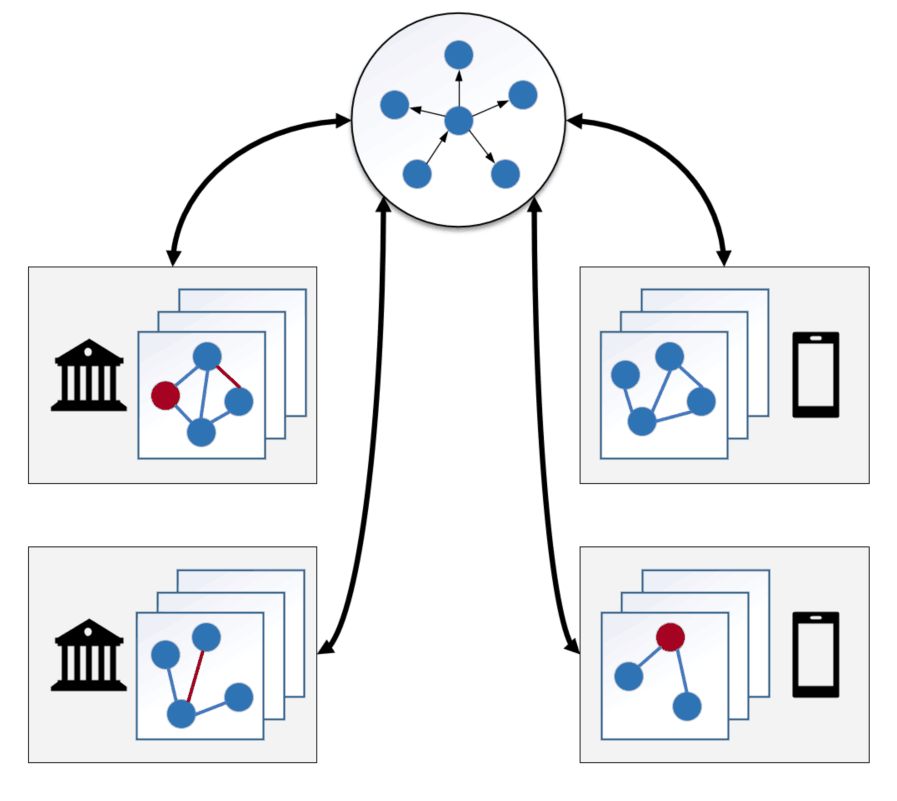
\includegraphics[width=0.5\textwidth]{1-1.png}
  \caption{跨域知识图谱的分布}
  \label{fig:1-1}
\end{figure}

传统的知识表示学习任务在训练集上学习知识图谱的嵌入表示,在测试集上获得实体或关系对应的向量并直接进行计算。而在跨域知识图谱上,目标域知识图谱存在着源域知识图谱中未定义的实体和关系,无法直接从源域知识图谱的嵌入中获取到对应的向量表示。同时出于用户隐私、成本等方面的考量,无法将新的实体和关系在源域知识图谱中进行知识融合并重新训练。因此跨域知识表示学习任务要求能够从源域知识图谱的训练中学习到对目标域知识图谱中未见实体和未见关系的表示。现有的基于逻辑规则的跨域知识表示学习方法通过自主学习逻辑规则来实现图谱嵌入,但其采用置信度来评估规则的质量,降低了规则的可信度,同时基于规则的模型也存在可扩展性差、大规模知识图谱训练效率低的问题。基于图神经网络的跨域知识表示学习模型聚合邻域特征对目标域知识图谱上新的实体和关系进行表示,但现有模型没有考虑到实体与关系的联系,并且在利用图结构信息进行嵌入的过程中,未能充分利用知识图谱的语义信息。

为了解决上述跨域知识图谱的表示学习上存在的问题,本文提出基于本体信息和元学习的知识表示学习方法。该方法通过对图谱结构信息和本体语义信息的特征学习,能够有效地嵌入表示目标域知识图谱上的新实体和新关系,为跨域知识图谱的表示学习提供一种新的解决方案。同时,本文采用元学习的方法在训练任务上模拟出未见的实体和未见的关系,使得模型能够通过多个训练任务快速收敛,并在测试任务上取得良好的效果。本文所提出的模型也可以应用于现实世界中的真实应用场景,具体流程为:首先在大规模源知识图谱上进行训练,找到最佳的模型参数;随后,利用该模型在各种低资源环境下对目标知识图谱进行小规模的图谱嵌入,以供下游应用如推荐系统、问答系统等使用。本文模型能够有效解决跨域知识图谱的表示学习问题,同时减小整个训练流程的成本消耗,提高源知识图谱的样本利用率。


% 典型的知识图谱通过人工和自动相结合的构建方式已经获得了大量的事实三元组,但仍旧是高度不完整的。以Freebase为例,作为当前最大的通用知识图谱之一,其中75\%的人物实体缺失国籍信息\cite{1022484779.nh}。因此知识图谱补全任务(Knowledge Graph Completion,KGC)受到了研究者广泛的关注,KGC通过预测新三元组的真实性对知识图谱进行补全。知识图谱的三元组存储方式虽然已经可以将知识进行高效的结构化表示,但是这种符号形式的表示仍旧会导致知识图谱在使用上备受局限。为了解决这个问题,知识图谱嵌入(Knowlege Graph Embedding,KGE)等的知识表示学习(Knowledge Representation Learning,KRL)方法的相关研究很快起步并获得了广泛的关注。KGE旨在将符号化的三元组(h,r,t)映射到低纬稠密的向量空间,便于实体和关系之间的计算\cite{2021-eh},降维后获得的知识图谱嵌入可以作为其他网络模型的输入来辅助下游任务的效果提升,包括知识图补全、三元分类、实体识别和关系抽取以及图谱外任务如推荐系统、问答,例如谷歌构建的规模庞大的知识图谱也已经展示出该方法的强大能力。

% 经典的KGE模型如基于翻译的TransE\cite{bordes2013translating}模型在同一空间向量中嵌入实体和关系,通过头实体和尾实体的平移操作来进行关系嵌入,时空复杂度低,但在建模复杂关系的场景下弊端也比较明显。为此TransE相关的扩展模型\cite{wang2014knowledge}也陆续被研究应用。其他的KGE模型如基于分解的模型DistMult\cite{yang2014embedding}、CompleEx\cite{trouillon2016complex}以及旋转模型RotatE\cite{sun2019rotate}等也都获得了广泛的应用。但传统的KGE方法基于图谱中固定的实体集和关系集学习图谱嵌入,不能处理训练图谱中不存在的新的关系和实体。在面对跨域的知识图谱,传统的KGE方法在源知识图谱上训练后无法直接应用到目标知识图谱上对新的实体和关系的进行嵌入。

% 现有的一些KGE模型通过几种不同的思路来处理KGC任务中非源知识图谱存在的部分。基于规则学习的模型从事实三元组中挖掘出能够满足规定置信度和支持度阈值的所有规则,这些规则通过对实体的抽象摆脱了对具体实体的依赖,从而可以作用在新的实体上。但规则的制定会很大影响到任务的效果,人工制定的规则质量好但成本高,通过自主学习规则的模型通过置信度来评估规则的质量降低了规则的可信度,并且基于规则的模型也存在可扩展性以及大规模知识图谱训练效率的问题。随着图神经网络(Graph Neural Networks,GNNs)的提出以及在知识图谱上的应用,基于图神经网络的嵌入模型成为知识表示学习的另一个主要趋势。GNNs通过节点的邻接点更新节点的状态,从而编码邻居节点信息和图的拓扑结构信息。这种聚合的方式使得GNNs模型具有天然可对目标知识图谱上新实体进行编码的能力。一些研究者通过GNN对链接预测三元组头尾实体的局部子图进行学习,在存在源知识图谱实体集未包含实体的新三元组的预测任务上也取得了一定的效果。但这些GNNs模型往往作用于新的实体,并没有考虑到新的关系,同时利用结构信息对新实体嵌入的过程中没有很好利用到像本体信息这种高度抽象的语义信息对表示学习进行增强。

% 为了解决上述在跨域知识图谱的表示学习上仍存在的问题,本文提出了一个基于GNN的知识表示学习框架。通过对图谱结构信息和本体语义信息的特征学习,能够对目标知识图谱上的新的实体和关系进行有效的嵌入表示,为跨域知识图谱的表示学习提供了一种新的解决方案。同时,本文通过采用元学习的方法在训练任务上模拟出未见的实体和未见的关系,使得模型能够通过多个训练任务的训练快速收敛,并在测试任务上取得良好的效果。在现实世界的应用中,可以采用本模型在大型的源知识图谱上进行训练,获得最优的模型参数,然后在各低资源的环境上,直接对目标知识图谱上进行小规模的图谱嵌入,可用于推荐系统、问答系统等下游应用等。能够有效解决跨域知识图谱的表示学习问题,同时减小整个训练流程的成本消耗,提高源知识图谱的样本利用率。

\section{国内外研究现状及趋势}
跨域知识表示学习一般涉及到融合辅助信息及基于归纳推理的知识表示学习方法。近几年,元学习在知识表示学习中也获得了众多学者的关注,主要用于在少样本、零样本等情境下对表示学习能力的加强。本节将阐述相关方法的研究现状及趋势。

\subsection{融合辅助信息的跨域表示学习方法}
传统的KGE方法主要包含基于翻译的表示学习方法和基于语义相似度的方法。基于翻译的方法通过测量低维向量间的距离来计算出三元组事实的可信度。这些方法通常会将关系的嵌入视为从头结点到尾结点的向量平移,代表模型有TransE\cite{bordes2013translating}及其变体如TransH\cite{wang2014knowledge}、TransR\cite{lin2015learning}等。基于语义相似度的方法通过比较实体和关系在向量空间表示中隐藏的语义特征的相似程度,来评判三元组的合理性,代表模型有DistMult\cite{yang2014embedding}、ComplEx\cite{trouillon2016complex}等。上述两类方法的本质都是通过设定的打分函数对图谱实体和关系的语义表示向量进行更新,使得表示向量可以更多地贴近源知识图谱中的事实。因此,在传统的、目标域知识图谱不存在源域未见实体和未见关系的知识表示学习上,传统的KGE方法能够取得很好的效果。然而,面向跨域知识图谱的知识表示学习,传统的KGE方法无法从源知识图谱中学习到新的实体和关系有关的语义信息,不能很好完成对新三元组的预测任务。

为了对目标域知识图谱中存在的未见实体进行更有效的特征学习,一些学者尝试引入其他辅助信息,以增加表示向量中的隐含特征。知识图谱除了采用事实三元组进行知识存储,还蕴含着其他的丰富信息用于加强知识表示学习,如关系路径信息、图结构信息等。也有一些研究者通过使用图谱外的信息,如文本描述信息等增强传统的KGE模型的表示能力。

NTN\cite{socher2013reasoning}模型最早在表示学习中引入实体的描述信息,该模型对实体进行嵌入时并没有采用随机初始化的方法,而是将实体的文本描述信息编码作为实体的表示向量。此后基于描述扩展的知识表示模型DKRL\cite{xie2016representation}试图改进TransE模型,使其能够进一步处理实体描述。DKRL通过将实体结构及实体描述相关的向量联合表示来作为实体嵌入。其中实体描述向量由描述文本经过连续词袋\cite{valverde2012link}编码器或卷积神经网络编码器获得。另一种常见的引入辅助信息的方法借助实体的关系信息来进行表示学习,关系信息揭示了实体之间的一个或多个语义联系。PtransE\cite{lin2015modeling}首次将图谱的多跳关系信息作为知识图谱嵌入的辅助信息使用,在TransE的基础上提出了一个以关系路径为基础的表示学习模型。PtransE的打分函数由两个部分组成,其中一部分是针对头尾实体直接相连关系路径的打分;另一部分是针对头尾实体间其他多跳关系路径的打分。这一改进使得TransE的单步推理得以扩展为多步推理,提升了在链接预测任务上的表现。冯俊等人则将知识图谱视为一个大的有向图,提出了基于图感知的表示模型GAKE\cite{feng2016gake},该模型利用知识图的结构信息来学习任意顶点或边的表示。
% \begin{figure}[h]
%   \centering
%   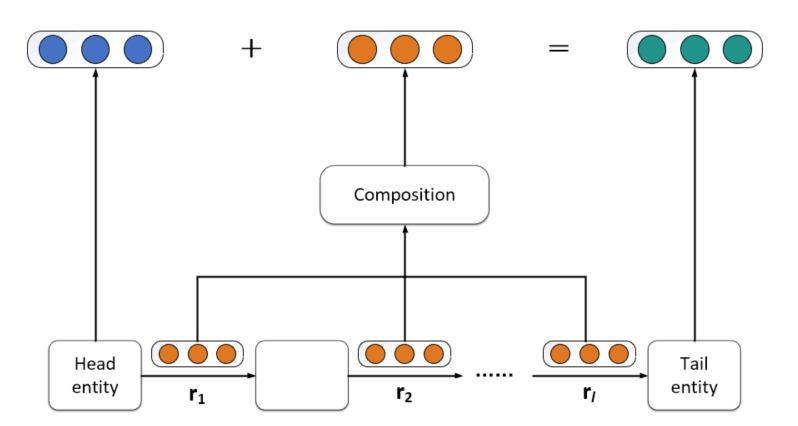
\includegraphics[width=0.7\textwidth]{1-6.png}
%   \caption{PtransE的模型架构}
%   \label{fig:1-6}
% \end{figure}

除了利用图谱自身隐含信息进行表示学习的方法外,一些学者还会引入外部知识以增强表示学习的效果。例如上述的实体描述信息,也可以从新闻稿或者维基百科中获取。图谱外其他模态的信息也同样适用于辅助表示学习,如实体的图像信息、自定义的语义证据等。代表性的IKRL\cite{xie2016image}模型实现了基于跨模态结构与基于图像的联合表示方法,该模型在遵循平移原则的基础上将图像编码到实体空间。IKRL提出的跨模态表示可以确保基于结构和基于图像的表示映射在同一个表示空间中。Ren\cite{li2022does}团队提出的基于语义证据的表示学习方法通过对语义证据的预测及实验验证,研究了KGE的外推问题,并通过建模实现了对三种语义证据的加强,在存在有未见实体的知识图谱补全任务上,相比于传统的KGE方法取得了更好的表现效果。

\subsection{基于归纳推理的跨域表示学习方法}
为了解决传统KGE方法无法处理目标域知识图谱中存在未见实体和未见关系的问题,学者们开始探索基于归纳推理的知识表示学习方法。这类方法通过对结构或一般规则的学习尽量减小对实体和关系的依赖,将表示学习能力泛化到对目标域知识图谱的新三元组的预测任务上。基于归纳推理的知识表示学习方法主要可分为基于逻辑规则和基于GNN的表示学习方法,本节将分别介绍两种方法的研究现状。

\paragraph{基于逻辑规则的表示学习方法}
基于逻辑规则的表示学习方法通过学习关系的共现模式来挖掘逻辑规则。从形式语言表达能力的角度可将规则分为“命题规则”和“一阶逻辑规则”\cite{2023-ed}。命题规则限定了具体的关系及实体,不包含变量,因此具有很强的限制性,无法应用到其他实体的推理任务上。一阶逻辑规则包含了关系及变量,可看作对命题规则的抽象,与具体的实体无关。这些规则从本质上获得了归纳推理的能力,摆脱了实体依赖的限制,可以对存在新实体和关系的三元组上的任务进行推理指导。

在对知识图谱事实三元组中隐含的规则进行挖掘上,传统的规则挖掘方法如AMIE\cite{galarraga2013amie}模型基于路径遍历的思想实现挖掘算法。这些模型将知识图的关系路径近似视为规则进行提取,通过统计度量或者固定的人工设定模式进行规则的学习。但是由于知识图谱的复杂关系,遍历路径会使得规则提取的成本大大提高,无法应用于大型知识图谱,并且这些传统的规则提取方法存在无法扩展的问题。

随着知识表示学习方法的广泛应用,基于表示学习的规则挖掘方法通过对实体和关系的向量打分来挖掘规则,典型的模型有RLvLR\cite{omran2018scalable}、HARL\cite{omran2022learning}、IterE\cite{zhang2019iteratively}等。RLvLR模型通过联合表示学习和子图采样方法从图谱中学习规则,能够在大型的知识图谱如Freebase、YAGO上进行有效的规则提取。HARL在RLvLR的基础上考虑了实体的属性信息,添加了对实体属性的规则学习。IterE模型为了获得对知识图谱中存在的大量稀疏实体和关系更准确的表示,提出了表示学习和规则学习同时进行的迭代算法。该模型在表示学习的基础上添加了公理归纳和公理注入的模块,通过对稀疏的实体和关系的公理注入来加强表示学习的效果,获得了规则和表示学习的共同提升。国内刘藤\cite{2021-qx}等人在IterE模型的基础上,专注于规则学习和规则融合模块的改进。他们基于三元组的打分函数,对规则置信度计算方法进行了改进,扩大了模型的适用性。此外,他们还实现了利用表示更新规则及利用规则增强表示的迭代算法,进一步提高了该方法的性能。

在专注于跨域知识图谱的链接预测任务上,一些可微规则学习方法如Neural-LP\cite{yang2017differentiable}模型和DRUM\cite{sadeghian2019drum}模型,采用端到端的方法学习规则逻辑。此类方法通过设计可微的逻辑规则学习模型,采用基于梯度的方法进行优化求解。然而这些方法不能解决知识图谱中缺边的问题,同时在处理候选规则中的不合理部分仍存在不足。不同于直接从事实三元组中学习逻辑规则的方法,一些方法利用子图隐式地表示逻辑规则。GraIL\cite{teru2020inductive}和TACT\cite{chen2021topology}通过学习未见实体周围的封闭子图结构,并将其用作逻辑规则。但是随着实体邻居数目的指数增长,这些子图的规模可能会很庞大从而导致效率低下的问题。

\paragraph{基于GNN的表示学习方法}
基于GNN的表示学习方法在传统的知识图谱嵌入方法上进行延伸,利用图神经网络作为编码器学习图结构信息,并采用TransE、ComplEx等传统知识图谱嵌入方法作为解码器。

Hamaguchi\cite{hamaguchi2017knowledge}等人将图神经网络应用到知识图谱上。不同于先前学者利用GNN将子图整体进行编码的方法,Hamaguchi利用图神经网络,将图中的实体和关系分别映射到单独的向量中。对于三元组中待预测的新实体,该方法通过汇总所有已知实体的信息来生成新实体的嵌入向量。该方法通过GNN编码节点信息和图的拓扑结构,能够处理跨域知识图谱中的未见实体,展现了GNN在知识图谱上的有效应用,催生了许多基于GNN的知识图谱嵌入方法的实现。然而,该方法在聚合邻居节点特征时,仅采用简单的池化操作,没有对邻居节点进行区分或引入关系特征。

图卷积网络\cite{kipf2016semi}(Graph Convolutional Network,GCN)是在图神经网络和卷积神经网络的基础上发展而来的。GCN通过在节点特征和邻居信息上进行卷积操作来更新节点表示,充分地进行邻居节点之间的信息传递。然而,GCN只适用于同构图,无法处理知识图谱中复杂的关系结构。而关系图卷积网络\cite{schlichtkrull2018modeling}(Relational Graph Convolutional Network,R-GCN)则为不同类型的关系设置不同的权重矩阵,将GCN模型扩展到了多关系图中。在此基础上,VR-GCN\cite{ye2019vectorized}在对实体和关系的嵌入过程中,考虑了知识图谱中不同关系方向和不同实体类型可能具有不同特征空间的情况。而TransGCN\cite{cai2019transgcn}则在VR-GCN的基础上,,利用RotatE思想对聚合函数进行扩展,提出了一种新的处理异构关系的方法。CompGCN\cite{vashishth2019composition}基于TransE、DistMult和HoIE的思想设置了三种不同的聚合操作,对图谱中的实体和关系信息同时进行建模和学习,并通过共享各层关系嵌入解决了过参数化的缺陷。

不同于上述模型对关系信息的关注和加强,受序列任务中注意力机制的启发,图注意力网络\cite{nathani2019learning}Graph Attention Networks,GAT)将注意力机制和图卷积网络结合,增加对邻接点关注度的区分,并应用于图数据中的节点分类。相关实验结果表明,该机制的引入可以高效地作用于跨域知识表示问题。此外,r-GAT\cite{chen2021r}(Relational Graph Attention Network)采用多通道的方法学习实体的嵌入表示,其中每个通道对应不同的实体语义信息,同时利用关系特征聚合邻居信息,从而能够有效处理复杂的多关系图。

\subsection{元学习在知识表示学习中的应用}
元学习的目的是帮助模型掌握如何学习的能力。其主要应用场景为数据稀少的零样本学习和小样本学习等,能够更快、更好地学习新的知识表示,并泛化至新的任务。

MetaR\cite{chen2019meta}模型首次将元学习应用到少样本的链接预测任务上。该模型尝试通过元学习的方法捕捉源域知识图谱中事实三元组隐含的、与关系相关的元信息。这类元信息通常是一类任务中常见且通用的信息,因此可迁移到新的三元组中。并且,通过使用小批量的三元组进行元学习,可以加速整个学习过程。MetaR结合元学习的方法解决少样本场景下的知识图谱补全任务,证明了元学习在跨域图谱的知识表示学习上的有效性。Meta-KGR\cite{lv2019adapting}模型提出了一种将强化学习与元学习结合的方法,以解决少样本的关系推理问题。该模型通过采用强化学习,训练了一个代理,用于搜索目标实体和多跳推理路径,从而提高了模型的可解释性。为了解决知识图谱补全过程中由于邻域稀疏导致的噪音过大问题,GANA\cite{niu2021relational}模型在MetaR模型的基础上引入了图注意力机制和门控网络对噪音进行过滤,同时采用TransH作为评分函数,提高了模型对复杂关系的表示能力。

随着图神经网络在知识表示学习中的良好应用,结合GNN和元学习方法的研究也受到了学者们的关注。Meta-iKG\cite{zheng2022subgraph}包含基于子图的元学习器。它将链接预测任务转换为子图建模问题,并采用局部子图传递子图特定信息。然而,该方法在对子图进行编码的过程中,仅提取了子图的结构语义,无法很好地处理反对称关系的三元组。最近提出的MorsE\cite{chen2022meta}同样结合了GNN和元学习方法,将元知识学习分为实体初始化器和图神经网络调制器两个模块。实体初始化器通过两个与实体无关的嵌入(关系域嵌入和关系范围嵌入)初始化每个实体嵌入。而GNN调制器则利用实体的邻居结构信息增强实体嵌入。通过对与实体无关的元知识进行建模和学习,MorsE可以为新实体生成高质量的嵌入。

整体而言,元学习方法侧重于捕获关系信息。模型整体结构分为两个部分:第一部分负责融合信息,获取任务相关的表示;第二部分利用元学习训练模型参数,从而将学习能力快速泛化到新关系上。为了满足具体任务的需要,这些方法往往会通过结合其他方法进行加强。

% 知识图谱表示学习的关键是学习出实体和关系特征的低纬度表示,这些表示空间主要是指逐点空间,具体的像向量、矩阵和张量等表现形式;而其他类型的表示空间,如复向量空间、高斯空间也被研究者所使用 \cite{dai2020survey}。基于翻译的方法通过测量实体向量间的距离来计算出三元组事实的可信度。这些基于翻译的方法通常会将关系的嵌入视为从头结点到尾结点的向量平移,例如Bordes等研究者在借鉴Word2Vec \cite{mikolov2013distributed}中的语义平移后提出的TransE模型认为在同一表示空间中头结点向量和关系向量的向量和在距离上应该更靠近事实上的尾结点,并以此设置评分函数进行图谱嵌入,在WordNet和FreeBase两个数据集上的链接预测任务的效果相比于早期的RESCAL \cite{nickel2011three}模型会更好。同时由于TransE模型结构并不复杂,实现简单,在学术界和工业界都获得了广泛的研究及使用,使其成为经典的知识表示学习方法之一。
% \begin{figure}[h]
%   \centering
%   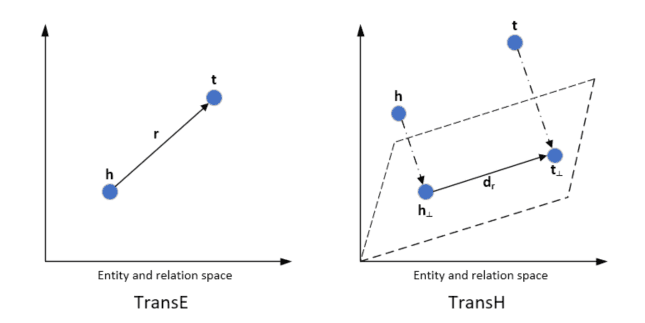
\includegraphics[width=0.8\textwidth]{1-2.png}
%   \caption{TransE和TransH的实体关系映射}
%   \label{fig:1-2}
% \end{figure}

% Bordes提出了关系的四种类型:1对1、1对多、多对1、多对多。TransE通过比较头结点与关系的向量和与尾结点的距离能够有效的处理1对1的简单关系类别,但同时缺点也显而易见,在处理复杂关系时由于实体或者关系嵌入的相似性会导致实验效果的下降。假设建模1对多的复杂关系,有(海贼王,人物,梦奇·D·路飞),(海贼王,人物,娜美)两个三元组,在同一个表示空间中,由于实体h和关系r相同,TransE会认为对应的所有尾实体都应该具有极为相似的向量表示,但很明显这个结论与事实相悖。为了弥补TransE模型的弊端,在该模型的基础上,相关的模型研究也有更新的发展。TransH通过将头尾实体都映射到关系的超平面上,即使头实体和关系一致也不会导致尾实体的嵌入一致,规避了尾结点重叠的问题,可以在一定程度上处理多对多的关系。
% \begin{figure}[h]
%   \centering
%   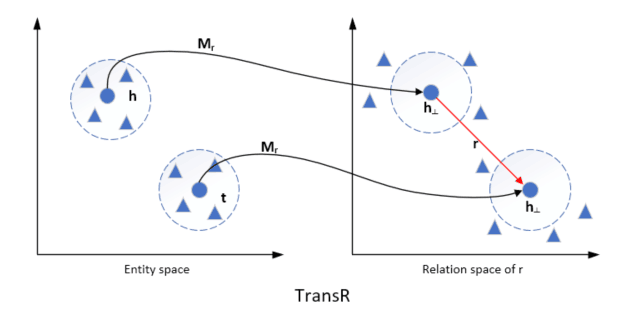
\includegraphics[width=0.8\textwidth]{1-3.png}
%   \caption{TransR的实体关系映射}
%   \label{fig:1-3}
% \end{figure}
% \begin{figure}[h]
%   \centering
%   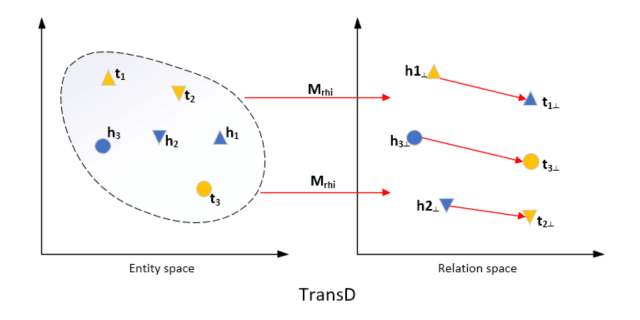
\includegraphics[width=0.8\textwidth]{1-4.png}
%   \caption{TransD的实体关系映射}
%   \label{fig:1-4}
% \end{figure}

% TransR \cite{lin2015learning}舍弃了实体和关系映射在统统一语义空间中的假设,把TransH涉及到的实体在关系上特有的映射的概念延展成关系特有的语义空间映射,在TransR的设定中三元组的实体映射到一个语义空间,而关系则表示为关系语义空间中的转换向量,TransR定义了关系关联的映射矩阵, 在执行转移操作之前, 分别通过实体向量在关系映射矩阵上的映射获得关系空间内的头实体与尾实体表示, 最后通过计算头实体映射向量加关系向量和尾实体映射向量的距离得到优化目标。但TransR模型将实体语义空间与关系语义空间的交互仅仅与关系矩阵相关联明显不合理,且由于空间投影使模型参数急剧增加,基于此Ji等人提出了TransD \cite{ji2015knowledge}模型,TransD模型设置了两个投影矩阵,分别将头实体和尾实体投影到关系空间,同时只利用两个投影向量构建投影矩阵来减少参数量。

% 总体上,基于翻译的Trans模型都将关系作为实体向量间的翻译,但受限于结构的弊端往往不能很好处理复杂关系的场景,无法得到蕴含更多特征的知识图谱表示。

% \subsection{基于语义相似度的方法}
% 基于语义相似度的方法通过标记实体和关系在向量空间表示所隐藏的语义特征的相似程度来作为评判三元组合理性的标准。传统的的语义匹配的模型一般采用张量分解的方式来完成,其中的张量由一个多维的数组来表示 \cite{kolda2009tensor}。
% \begin{figure}[h]
%   \centering
%   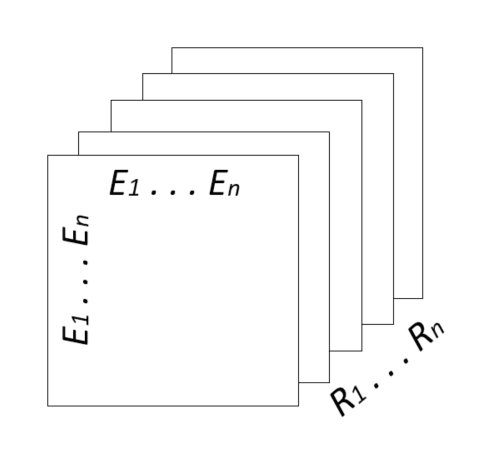
\includegraphics[width=0.5\textwidth]{1-5.png}
%   \caption{知识图谱的张量模型}
%   \label{fig:1-5}
% \end{figure}

% RESCAL模型将每个实体与一个向量联系起来,以捕捉其潜在的语义。每一种关系都用一个矩阵来表示,该矩阵模拟了潜在因素之间的双向相互作用。该模型通过潜在特征的成对交互解释三元组,首先将知识图谱中的三元组转换为三维张量\(X\)。给定一个张量\(X \in R^{n×n×m}\),其中\(n\)和\(m\)分别表示实体和关系的数量,该张量的两个模保存连接的头尾实体,另一个模则保存关系。如果一个张量实体\(X_{ijk} = 1\)即表明知识图谱中存在三元组(第i个实体,第k个关系,第j个实体);否则,\(X_{ijk} = 0 \)表示不存在或未见的三元组。然后对张量的每一个切片(关系数据)执行分解来获得实体的潜在语义表示,然而该模型的主要缺点在于对频繁出现的关系表现的很好,但对少见的关系表现的很差,并且容易导致过拟合,不适用存在大量稀有关系的数据集 \cite{choudhary2021survey}。鉴于此,研究者提出了一个潜在因子模型TATCE \cite{garcia2014effective},它能够将高容量三向模型与更易于控制的双向交互模型相结合,并利用它们两者的优势。由于双向和三向模型不使用相同的数据模式,也不在嵌入中编码相同的信息,因此在TATEC中,他们在第一阶段使用了两种不同的嵌入,然后在后期将它们组合并微调。相比于三向模型RESCAL、传统双向模型TransE以及同样采取双向三向模型结合的NTN \cite{socher2013reasoning}模型等,在链接预测任务上TATEC表现更优。为了简化模型计算的复杂度,DistMult模型在RESCAL的基础上将关系矩阵简化为对角矩阵,从而减少双线性模型的参数量,达到和TransE基本相同。ComplEx模型是对DistMult在关系模式上的改进,不仅具有学习对称关系的能力,还能够提供一些非对称性的表示。

% 近几年随着神经网络的兴起,由于其具有强大表示和泛化能力,也可以表达复杂的非线性投影。结合神经网络将知识图嵌入到连续的特征空间成为一个热门方向。其中代表性的如ConvE\cite{dettmers2018convolutional}、ConvKB\cite{nguyen2017novel}模型等,这些早期的结合神经网络模型的KGE方法采用卷积神经网络进行特性提取及嵌入,通过卷积神经网络捕捉知识库中的全局关系和翻译特性。将三元组输入到卷积层中进行卷积操作,输出特征并拼接为特征向量,然后经由评分函数进行打分。随着图卷积模型\cite{kipf2016semi}的提出及效果的不断提升,以图卷积网络为基础的KGE模型开始占据主流。R-GCN\cite{schlichtkrull2018modeling}首次提出采用图卷积网络做图谱嵌入任务,使用GCN的信息传播的思想表示图谱,并用上层的卷积输出作为下层的卷积输入。虽然R-GCN 的效果提升都比较微弱,但是因为GCN的出现,用它来做知识图谱表示学习也成为是一种必然。此后,基于GCN的KGE模型如CompGCN\cite{vashishth2019composition}也已经取代传统的神经网络KGE模型,不断取得更好的知识图谱嵌入效果。

% \subsection{融合辅助信息及归纳推理的方法}
% 基于翻译的表示学习方法和基于语义相似度的表示学习方法通过三元组信息学习实体及关系的表示。这些方法的目的都是学习知识图谱存储的事实信息并映射到嵌入向量中,使嵌入向量能够更好地贴近这些事实,从而完成各种下游任务。然而,这些仅依赖于知识图谱三元组进行表示学习的方法存在明显的弊端。这些学到的嵌入表示只能处理知识图谱中可见的实体和关系,对于未见组件可靠性会大幅下降。为了能够对这些未见的组件进行有效的特征学习,研究者往往会引入除三元组之外的辅助信息。因为知识图谱不仅通过三元组进行数据存储和检索,还蕴含着丰富的其他信息可以辅助进行知识图谱表示学习,比如文本描述信息、关系路径信息及图结构信息等。

% NTN模型最早在表示学习中引入实体的描述信息。虽然该模型是利用图谱存储的实体的文本信息来对实体嵌入进行初始化操作。此后描述扩展的知识图谱表示模型DKRL \cite{xie2016representation}试图通过改进TransE模型使其能够进一步处理实体描述,DKRL将实体嵌入由实体结构相关的变量及实体描述相关的变量联合表示,其中实体描述变量由描述文本通过连续词袋 \cite{valverde2012link}编码器或卷积神经网络编码器获得的词嵌入构成。另一种常见的辅助信息通过借助实体的关系信息来进行表示学习,关系信息揭示了实体之间的一个或多个语义关系。PtransE \cite{lin2015modeling}首次将图谱的多跳关系信息作为知识图谱嵌入的辅助信息,提出了一个以关系路径为基础的表示学习模型。该模型在TransE基础上改进,模型打分函数由两个部分组成,一方面是头尾实体直接关系的打分,另一方面计算头尾实体间其他多跳关系路径的打分。从而将transE的单步推理扩展为多步,获得了不错的效果提升。冯俊等人则将知识图谱视为一个大的有向图,提出了基于图感知的表示模型GAKE \cite{feng2016gake}。该模型利用知识图的结构信息生成实体和关系的表示。
% \begin{figure}[h]
%   \centering
%   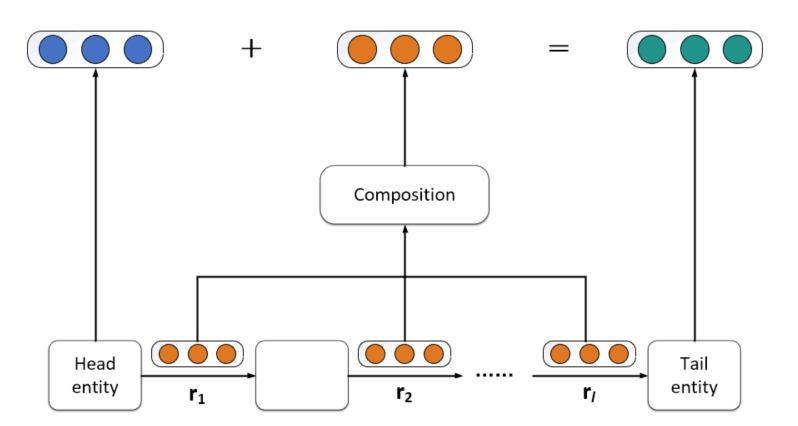
\includegraphics[width=0.7\textwidth]{1-6.png}
%   \caption{PtransE的模型架构}
%   \label{fig:1-6}
% \end{figure}

% 除了知识图谱自身的额外信息作为辅助外,许多研究者也会引入图谱外的其他知识用于表示学习。比如上述的实体描述信息,也可以从新闻稿或者维基百科中获取。图谱外其他模态的信息也同样被用于辅助表示学习,比如实体的图像信息,代表性的IKRL \cite{xie2016image}模型实现了包含基于跨模态结构和基于图像的表示,将图像编码到实体空间同时遵循平移原则。该模型提出的跨模态表示可以确保基于结构的表示和基于图像的表示映射在在同一个表示空间中。

% 以往的知识图谱表示学习聚焦于如何从现有的图谱知识中学习到更贴近知识的嵌入表示来完成相关的预测、补全、问答等任务,但这些学习往往学习到的不是更全局的表示,仅在现有的可见的图谱任务上才能获得较好的效果。而跨领域跨设备的场景要求更加苛刻的表示学习效果,需要更高层次、更适用性的知识提取,因此现有的研究开始向通用性知识以及辅助知识提取方向发展,该方向研究正在起步但无疑是未来的主要方向,本文的研究目标即在高层本体语义信息的辅助下进行更普适性的知识图谱表示学习。

\section{本文主要研究内容}
对于跨域知识图谱的知识表示学习,传统的知识图谱嵌入方法由于学习固定三元组的实体嵌入,无法很好地处理目标域知识图谱中的新实体和新关系。现有的基于归纳推理的模型尽管取得了一些效果,但利用逻辑规则的方法无法挖掘实体和关系间复杂的语义相关性;利用图结构信息对实体和关系进行嵌入的方法没有充分利用到未见实体与关系的相关性,且未考虑知识图谱语义信息(如本体)对表示学习的补充。一些学者尝试利用实体类型等辅助信息来增强表示学习,但这些信息往往集中于局部的特征。考虑到知识图谱本体可以提供更加丰富且完整的语义信息,包括实体类型、层次信息和关系信息,本文提出了一个本体信息增强的跨域知识表示学习模型,能够结合图的拓扑结构信息和本体语义信息对未见实体和未见关系进行建模,同时从实例关系位置结构中获得了关系本体三元组,结合本体描述文本对本体嵌入中的关系信息进行加强。

为了能更好的将源域的知识迁移到目标域,实现更好的泛化能力,本文提出了一种基于元学习的方法,将训练集划分成多个训练任务,并在每个任务中通过标签模拟未见实体和关系,以提高对目标域知识图谱上新实体和新关系的泛化学习能力。最后,本文进行了充分的实验和分析,验证了模型的有效性。

% \begin{enumerate}[label=\arabic*)]
%   \item 传统的知识图谱嵌入方法无法很好地建模跨域知识图谱嵌入中未见实体和未见关系。基于归纳推理的模型仅从子图结构来学习新实体和关系的表示,未能充分利用知识图谱其他语义信息。

%   \item 跨域知识图谱的知识表示学习要求模型能够在源域知识图谱上训练获得参数,并能够将学习能力迁移到存在新实体和关系的目标域知识图谱嵌入上。在跨域知识图谱场景下,需要保证模型对未见实体和关系的泛化学习能力。
% \end{enumerate}

% 本文通过对近几年相关技术的研究认为,本体作为知识图谱最高层次的语义抽象可以作为所有设备的全局信息,可以用于对未见关系和未见实体进行一定程度上语义特征的补充。同时借助于关系的位置关系,通过实体三元组关系与关系的相对关系构建出关系位置图,然后在该图中嵌入本体的语义信息,能够对关系节点进行编码从而学习到未见关系的特征表示;然后基于实体及连接关系的结构信息,可以通过未见实体连接的所有关系,聚合这些关系的特征作为实体特征从而实现了对未见实体的表示;最后,为了模拟出存在未见关系及未见实体的训练场景,本文借用元学习的思想设计了多个训练任务学习到最好的模型参数并进行实验验证了模型的有效性。

% 本文通过对近几年相关技术的研究认为,本体作为知识图谱最高层次的语义抽象可以作为所有设备的全局信息,并可用于对未知关系和实体进行一定程度的语义特征补充。此外,通过确定关系的相对位置关系,可以构建关系位置图,并嵌入本体的语义信息,从而对关系节点进行编码,以学习未见关系的特征表示。而后,基于实体及连接关系的结构信息,可以聚合连接未知实体的所有关系的特征,以表示未知实体。最后,为了模拟出具有未知关系和实体的训练场景,本文借用元学习的思想设计了多个训练任务,以学习最佳模型参数,并通过实验验证了模型的有效性。

% 许多学者已经尝试利用文本描述、属性描述、实体类型等多种辅助信息来增强实体和关系的表示,但这些信息往往集中于局部的特征,如实体类型仅强调类之间的层次关系。相比之下,知识图谱本体可以提供更加丰富且完整的语义信息,包括实体类型、层次信息和关系信息。因此,本文设计了一个本体信息增强的跨域知识表示学习模型。为了更好地建模未见关系,模型使用本体特征丰富关系的语义信息,同时利用关系间的相对位置构建关系位置图,以学习关系的结构信息。对于未见实体,本文通过聚合实体邻域的关系特征作为初始化表示,采用复杂图卷积网络对图上所有的实体和关系表示进行更新,得到了最终的向量表示。此外,为了模拟目标域知识图谱中存在未见关系和未见实体的场景,本文采用了元学习思想设计了多个训练任务,以获得对未见实体和关系的泛化学习能力。最后,本文进行了充分的实验和分析,验证了模型的有效性。

综上,本文的主要工作包括:
\begin{enumerate}[label=\arabic*)]
  \item 提出了一种嵌入学习模型框架,采用元学习的模型训练方法,分别训练多个单任务,并在各个训练任务中通过标签模拟未见实体和关系。在源域知识图谱上训练模型,并将训练的参数用于目标域的图谱嵌入上,实现了跨域知识表示学习任务。
  \item 针对目标域知识图谱上的未见关系,构建了一个以关系为结点的视图,融合本体信息和结构信息对关系进行建模,并基于关系拓扑结构和本体描述文本对本体嵌入加强。
  \item 在多个数据集上进行了充分的实验并与其他基准模型进行对比分析,实验结果表明了模型的有效性。同时通过一系列消融实验,证明了模型各部分的重要性。
\end{enumerate}

\section{本文组织结构}
本文的内容分为六章,以下主要概括各章的内容:

第一章,绪论部分:主要介绍跨域知识图谱的知识表示学习相关研究,探讨其现实意义,阐述了国内外学者在融合辅助信息、基于归纳推理的知识表示学习和元学习等方面的研究进展。最后概括了当前研究所面临的问题,并提出了解决思路。

第二章,跨域知识图谱的知识表示学习关键技术研究:分三个小节介绍本文模型主要涉及到的三种技术的发展状况及原理分析。其中,本体嵌入作为模型主要的语义信息补充,介绍了现有的本体嵌入方法。本文模型作为基于GNN的表示学习方法的实现,介绍了基于GNN的跨域知识表示学习模型所涉及的关键技术。最后简要介绍了元学习的主要技术及相关思想。

第三章,基于关系拓扑结构及描述文本的本体信息嵌入:介绍了如何捕捉本体的语义信息,并进行本体三元组的嵌入。为了补充本体中关系相关的三元组,本文采用了两种方法进行关系相关本体三元组的提取。在本体三元组结构嵌入的基础上,本章还详细说明了如何使用本体描述文本来增强本体嵌入。

第四章,基于元学习本体增强的跨域知识表示模型:详细介绍了本文提出的跨域知识表示学习模型的各个组成部分,主要包括未见关系嵌入、未见实体嵌入以及基于元学习的训练任务设定。为了验证知识表示学习模型的有效性,介绍了基于链接预测任务的模型实现流程。

第五章,实验结果及分析:介绍了本文使用的跨域表示学习效果评测所需的两个数据集的构建方法。在目标数据集上,对本文模型和相关基准模型进行了充分的实验,并分析实验结果,验证了模型的有效性。同时进行消融实验,对本文模型的各组成模块进行了验证,证明了各个模块的重要性。

第六章,总结部分:综合全文的研究内容及实验结果,总结了本文的主要工作,并对未来的工作进行规划。

% 本文的内容分为五章,以下主要概括各章的内容及安排:

% 第一章,绪论部分:主要介绍跨设备下的知识图谱表示学习相关的研究背景和现实意义,结合国内外研究者的相关研究分别介绍了传统的知识图谱表示学习方法中的基于翻译和基于语义相似度的方法以及相关一些通过辅助信息和归纳推理解决未见组件的一些研究进展,最后总结了研究面临的问题及本文的解决思路。

% 第二章,相关技术研究:分三个小结介绍了本文模型主要涉及到的三种技术的发展状况及原理分析。其中本体信息作为本文模型主要的语义信息来对未见组件进行语义层次的补充;元学习训练方法已经被广泛运用在各个领域,本文介绍了涉及到的设计方法;最后本文模型作为归纳推理模型的延伸,介绍了归纳推理模型相关的研究进展。

% 第三章,基于元学习本体增强的跨领域知识图谱表示模型介绍:详细介绍了本文提出的知识图谱归纳表示学习模型的各个组成部分,主要包含了本体信息嵌入模块、关系结构图构建及基于GCN的关系特征学习、基于CompGCN的实体特征学习模块。学习到实体和关系的相关表示后采用多种KGE得分函数来进行打分和更新。最后说明了模型在进行元学习训练的任务设定及训练流程。

% 第四章,实验结果及分析:介绍了本文采用的可用于归纳推理知识表示学习任务评测的三个数据集的构建方法以及相关用于本体嵌入的本体三元组抽取的方法。本章将本文模型及相关基准模型在目标数据集上进行了充分的实验并比较实验结果,验证了模型的有效性。最后对本文模型的各组成模块进行消融实验,验证了各模块的重要性。

% 第五章,总结部分:综合全文的研究内容及实验结果,总结了模型的可取部分及仍存在的问题与可改进的方法,对未来的相关工作进行规划。
\chapter{跨域知识图谱的知识表示学习关键技术}
传统的知识图谱嵌入模型通过提取三元组中的事实特征来对实体和关系进行编码。这类模型设计了评分函数如TransE、RESCAL等对三元组进行打分。然而在跨域知识图谱的场景下,目标域知识图谱存在新的实体和关系,传统的嵌入模型不能很好地学习到这些实体和关系的表示。基于规则和归纳推理的方法从子图或关系结构中学习向量表示,未能充分利用知识图谱的语义信息。为了解决跨域知识表示问题,本文设计了一个基于本体信息和元学习的跨域知识表示学习模型。本章将介绍模型涉及到的本体嵌入方法、基于GNN的表示学习方法以及元学习相关的关键技术。

\section{跨域知识图谱的知识表示学习定义}
知识图谱由众多的事实三元组组成,通常可以被定义为\(\mathcal{G} = (\mathcal{E},\mathcal{R},\mathcal{T})\),其中\(\mathcal{E}\),\(\mathcal{R}\),\(\mathcal{T}\)分别指代图谱实体的集合、关系的集合和实体三元组的集合。事实三元组中头尾实体和关系分别来自于实体集\(\mathcal{E}\)和关系集\(\mathcal{R}\),即\(\mathcal{T}=\{(h,r,t) \subseteq \mathcal{E} \times \mathcal{R} \times \mathcal{E}\}\)。传统的知识图谱表示学习旨在将实体和关系映射到连续的低维向量空间,同时保留知识图谱的结构特征。为了验证知识表示学习的有效性,一般会评价其在下游任务的性能表现,并将三元组划分为用于模型参数学习的三元组\(\mathcal{T}_{support}\)及用于测试的三元组\(\mathcal{T}_{query}\)。如在尾结链接预测任务中,给定测试三元组中的一个事实\((h,r,t) \in \mathcal{T}_{query}\),通过模型计算其所有可能的候选三元组\(\{(h,r,e) | e \in \mathcal{E}, (h,r,e) \notin \mathcal{T}_{support} \cup \mathcal{T}_{query}\}\)的排名,在所有预测三元组中,事实三元组\((h,r,t)\)的排名越靠前,则表明该表示学习模型的效果越好。

在跨域知识图谱的现实场景中,需要将源知识图谱上训练的模型应用于目标知识图谱上。由于成本、用户数据隐私等限制,无法将目标知识图谱与源知识图谱合并后重新训练,因此划分出跨域知识图谱。其中\(\textbf{源域知识图谱}\)包含大量已知事实三元组用于训练,\(\textbf{目标域知识图谱}\)作为源域知识图谱子集可能包含未定义的实体和关系用于测试。现给定一个用于训练的源域知识图谱\(\mathcal{G}^{train} = (\mathcal{E}^{train})\),并以在源域知识图谱上进行模型参数的学习为目标任务,从而能够将该模型应用在包含未见实体和未见关系的目标域知识图谱上,即\(\mathcal{G}^{test} = (\mathcal{E}^{test},\mathcal{R}^{test},\mathcal{T}^{test}_{support},\mathcal{T}^{test}_{query})\)。跨域知识图谱中的实体集和关系集遵循\((\mathcal{E}^{train} \neq \mathcal{E}^{test},\mathcal{E}^{train} \cap \mathcal{E}^{test} \neq \emptyset)\)及\((\mathcal{R}^{train} \neq \mathcal{R}^{test},\mathcal{R}^{train} \cap \mathcal{R}^{test} \neq \emptyset)\)。其中\(\mathcal{T}^{test}_{support}\)只用于标记测试集中实体与关系的结构,不用于对模型的训练。
\section{本体嵌入关键技术}
本体图是一种特殊的知识图谱,本体规定了一系列基本概念之间的语义关系。通常本体以层次概念为主干,通过属性来描述概念的语义关系,以表示通用或特定领域的知识。随着知识表示学习的不断发展,传统基于三元组结构信息进行表示学习的方法在面对跨域知识图谱等场景下,存在一定局限性。因此,越来越多的方法尝试引入本体信息,以提高表示学习的效果。如图\ref{fig:2-1}所示,这些本体信息不仅描述实体或关系的限制条件,如属性域和取值范围等,也是对知识图谱语义信息的抽象和集中表示。
\begin{figure}[h]
  \centering
  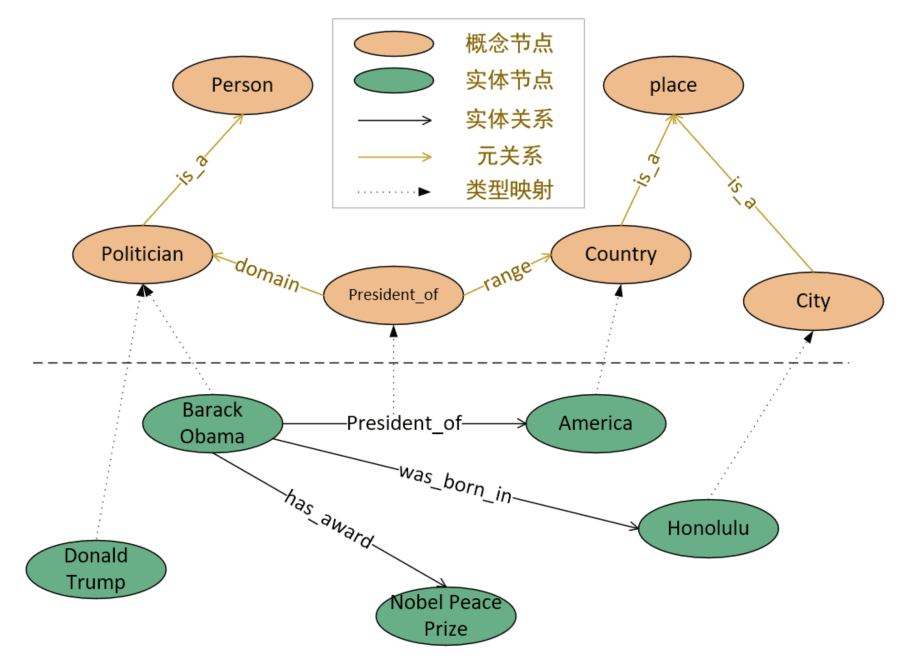
\includegraphics[width=0.8\textwidth]{2-1.png}
  \caption{知识图谱的本体视角和实例视角}
  \label{fig:2-1}
\end{figure}

本体图包含概念和概念间的元关系,通常被定义为\(\mathcal{G} = (\mathcal{C},\mathcal{P})\),其中\(\mathcal{C}\)是概念的集合,\(\mathcal{P}\)是元关系的集合。类似于实体三元组,一个本体三元组(s,r,t)表示概念s,t通过元关系r进行联系。然而,与实例知识图谱复杂多样的关系不同,元关系可进一步分类为传递关系、对称关系、层次关系和其他简单关系\cite{chen2018on2vec}。受KGE方法的启发,On2Vec\cite{chen2018on2vec}尝试将本体概念和元关系映射为低维向量。但该模型认为本体关系大多具有传递、对称等特性,不能直接将KGE方法应用在本体图上。例如对称关系r的两个三元组(c$_{1}$,r,c$_{1}$)和(c$_{1}$,r,c$_{1}$),当采用TransE等方法学习嵌入时,无法同时兼顾三元组对应的向量满足\(\textbf{c}_{1,r} + \textbf{r} ≈ \textbf{c}_{2,r}\)和\(\textbf{c}_{2,r} + \textbf{r} ≈ \textbf{c}_{1,r}\)。为了解决上述问题,On2Vec通过设置两个关系特定的投影函数,来区分同一概念在特定关系头尾位置的不同编码,如公式\ref{eq:2-1}所示:
\begin{equation}
  S_{d}(T) = || f_{1,r}(\textbf{s}) + \textbf{r} -f_{2,r}(\textbf{t})||,\label{eq:2-1}
\end{equation}
其中\(f_{1,r}\)和\(f_{2,r}\)分别代表了对特定关系r的三元组作为头本体和尾本体不同的投影操作。通过对头部本体和尾部本体分别进行不同的投影,可以解决上述传递元关系和对称元关系引起的矛盾问题。对于头尾本体投影操作的选择,On2Vec采用了简单的线性变换处理,如公式\ref{eq:2-2}所示:
\begin{equation}
  \begin{aligned} 
    &f_{1,r}(\textbf{s}) = \textbf{M}_{1,r}\textbf{s}, \quad\textbf{M}_{1,r} \in \mathbb{R}^{k \times k}, \\
    &f_{2,r}(\textbf{s}) = \textbf{M}_{2,r}\textbf{s}, \quad\textbf{M}_{2,r} \in \mathbb{R}^{k \times k},
    \end{aligned} \label{eq:2-2}
\end{equation}

特别对于层次关系,On2Vec将层次关系进一步划分为R$_{r}$和R$_{c}$,R$_{r}$表示粗略概念被划分为更细致概念的细化关系,而R$_{c}$表示将更细致概念分组为更粗略概念的简略关系。该模型为使细致概念的嵌入汇聚在一个更紧密的邻域内,采用层次模型对层次关系进行单独的处理。对层次关系嵌入的评分函数设置如公式\ref{eq:2-3}所示:
\begin{equation}
  \begin{aligned} 
    S_{hm}(G) = &\sum_{r\in R_{r}} \sum_{s\in C} \sum_{r\in \sigma(s,r)} \omega(f_{1,r}(\textbf{s}) + \textbf{r},f_{2,r}(\textbf{t}))\\
    + &\sum_{r\in R_{c}} \sum_{t\in C} \sum_{r\in \sigma(t,r)} \omega(f_{2,r}(\textbf{t}) -\textbf{r},f_{1,r}(\textbf{s})),
    \end{aligned} \label{eq:2-3}
\end{equation}
其中,\(\omega\)为两个参数向量的角度或距离单调递增的函数,On2Vec采用余弦距离函数。\(\sigma\)为对相应层次关系的本体节点的搜索操作,包括对细化关系寻找所有该关系下的所有尾本体、对简略关系寻找该关系下的所有头本体。On2Vec扩展了TransE方法,通过捕获本体关系的关系属性和层次结构,实现了对本体概念和元关系的表示,同时证明了在本体图上应用知识图谱嵌入方法的有效性。

现有的大多数本体模型在知识嵌入过程中都只包含单一的本体信息,对表示学习的补充作用有限,如SSE\cite{guo2016sse}、TKRL\cite{xie2016representation-TKRL}都仅采用了本体中实体类型信息,无法实现对所有可用本体信息的嵌入。本文能够在知识嵌入过程中整合所有可用的本体信息,充分补充图谱,提高复杂场景下的决策能力。同时本文使用了一种简单的本体形式,即RDF模式(RDF Schema,RDFS),而那些更复杂的OWL本体可以按照一定的标准转换为RDFS本体。

\section{基于GNN的跨域知识表示学习关键技术}
图神经网络模型是专门用于处理图数据的模型,对图结构进行编码,并进行节点级别、边级别及图级别的预测任务。CNN模型只能作用在具有相同结构的图像或者特定序列的语音和文字上,而图数据没有固定的形式且邻居节点也都是无序的,因此CNN模型无法作用在复杂的知识图谱上。相比之下,GNN通过聚合和更新操作,能够学习到图谱结构和节点特征的有效信息。

为学习到图的结构信息和节点特征,GNN主要包含了两个部分:聚合函数和更新函数。聚合函数可以将相邻节点的特征进行聚合,可以使用诸如sum、mean和max等聚合操作。一次聚合操作可以提取邻接节点的信息,这些邻接节点距离当前节点为一跳。GNN通常包含多层,每一层都会用上一层的信息进行聚合和传递。因此,n层聚合后传递的信息包含了n层邻接节点的结构信息和节点本身的特征信息。每层的特征聚合函数,如公式\ref{eq:2-7}所示:
\begin{equation}
  h_{v}^{k} = \sigma(W_{k} \sum \frac{h_{u}^{k-1}}{|N(v)|} + B_{k}h_{v}^{k-1}) \quad where \quad k = 1, ..., k-1 \label{eq:2-7}
\end{equation}
其中本层输出特征\(h_{v}^{k}\)包含两个组成部分。\(W_{k}\sum\frac{h^{k-1}_{u}}{|N(v)|}\)表示邻接点特征的聚合操作,后一部分是上一层聚合的特征与本层权重参数的乘积。这两部分特征通过激活函数更新,输出本层节点的特征表示。在GNN模型中,聚合函数没有区分邻接节点的重要性,仅采用简单的池化操作。

基于GNN的一种改进方向为集中于对图中关系表示的补充。图神经网络关注节点特征的聚合和更新操作,但在信息传递的过程中,图的关系结构仅用于指明邻接点,关系特征未参与节点的更新过程。为了增加关系信息对节点的影响,R-GCN在每层节点特征计算中引入了邻接点间的对应关系,更新函数如公式\ref{eq:2-8}所示:
\begin{equation}
  h_{i}^{l+1} = \sigma \left( \sum_{r\in\mathcal{R}} \sum_{j\in\mathcal{N}_{i}^{r}} \frac{1}{c_{i,r}}W_{r}^{l}h_{j}^{l} + W_{0}^{l}h_{i}^{l}\right), \label{eq:2-8}
\end{equation}

与GNN对邻接点特征聚合的操作不同,R-GCN引入了关系特定的转换。这种转换取决于边的类型和方向。为确保第l层的节点表示可以受到自身层次表示的影响,R-GCN在基础的图关系上为每个节点添加了一个自连接的特殊关系。如图\ref{fig:2-2}所示,在R-GCN中每层对一个实体节点(红色块表示)进行特征生成的过程中,首先从邻接点获取特征(蓝色块表示)并根据该节点与邻接节点的关系类型进行特征转换得到该种关系对应的表示(绿色块表示),其中关系类型分别由入关系、出关系以及自循环关系组成。然后将所有根据关系类型转换后的邻接节点信息累加求和,并通过一个如ReLU的激活函数更新,即可获得该节点本层的输出表示。相比于R-GCN,近期提出的CompGCN在R-GCN模型的基础上进一步引入了注意力机制,针对每种边类型和方向分别进行了注意力计算以加强对重要信息的关注。而且在计算效率方面,它减少了每个节点的嵌入大小及依赖于固定卷积核的计算量,因此更适合于大规模图数据。
\begin{figure}[h]
  \centering
  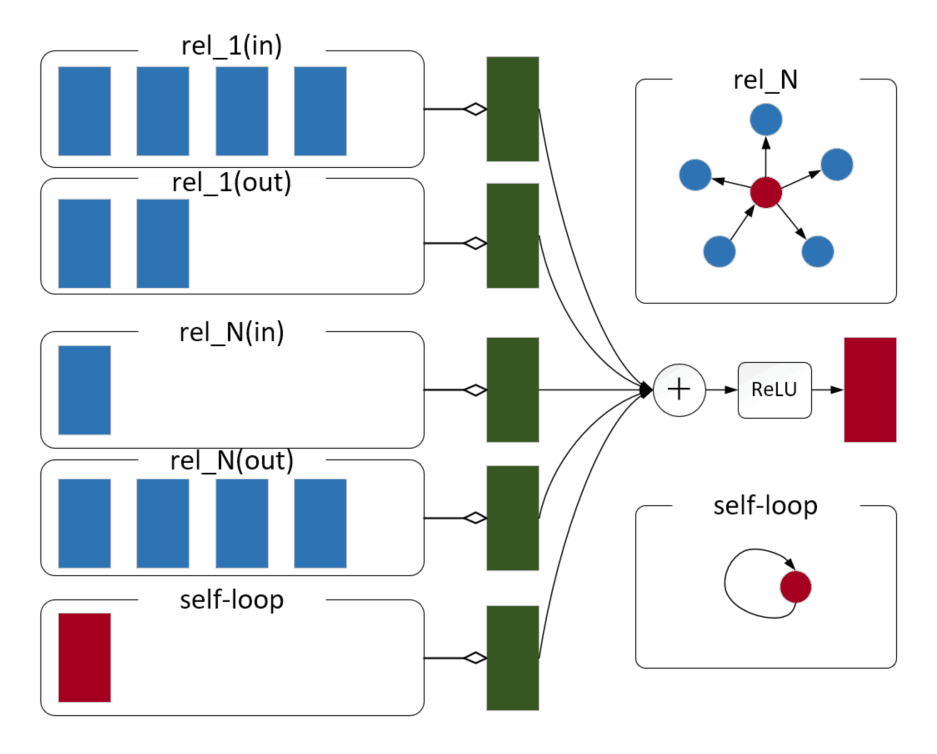
\includegraphics[width=0.7\textwidth]{2-2.png}
  \caption{R-GCN的特征传递}
  \label{fig:2-2}
\end{figure}

图神经网络通过聚合实体的邻域信息进行表示学习,一定程度上已经可以处理跨域知识表示问题,许多方法将GNN与其他方法结合进一步加强跨域知识表示学习效果。例如,INDIGO\cite{liu2021indigo}模型使用实体三元组与GNN的内层和外层的特征向量元素之间的一一对应关系对知识图谱进行编码,并避免了额外的打分函数,充分利用了GNN的特征聚合能力。其他方法如Zhao\cite{zhao2020attention}等人通过基于注意力的图网络聚合未见关系的邻接结构特征,来作为未见关系的表示。但这些方法要么专注于传统的知识表示学习领域,要么通过结构信息对未见的实体或关系进行嵌入,忽略了图谱的语义信息。本文通过全局本体信息的嵌入表示,在加强知识引入的同时,借助关系的位置结构信息来训练一个兼顾未见实体和关系的基于GNN的表示学习模型。

\section{元学习训练方法}
元学习最普适性的算法思想可以理解为“learning to learn”,它通过多个学习任务的训练来改进学习算法,而传统的机器学习算法则是在多个数据实例上进行模型的学习。

传统的机器学习方法会设置一个训练集\(\mathcal{D} = \{(x_{1},y_{1}),...,(x_{N},y_{N})\}\),如样本对(输入的图片,图片的标签)。而元学习的目的是训练出一个模型函数\(y = f_{\theta}(x)\),通过训练来获得其中的参数\(\theta\),求解公式如公式\ref{eq:2-9}所示:
\begin{equation}
  \theta^{*} = \underset { \theta } { \operatorname { arg } \operatorname { min } }\mathcal{L}(\mathcal{D};\theta,\omega) \label{eq:2-9}
\end{equation}
其中的\(\mathcal{L}\)是一个用于计算真实标签与模型预测标签之间的误差的损失函数,\(\omega\)指代了模型如何学习的假设,例如如何为参数\(\theta\)选择合适的优化器或者为\(f\)选择函数类型等。传统的机器学习方法实现过程中,该部分由研究者手动设置。模型的泛化性能则通过评估模型在已知标签测试集上的任务性能来衡量。传统的机器学习假设模型的优化在每个训练集\(\mathcal{D}\)上由初始参数开始执行,模型如何学习的设定是预先指定的,而这些设定将极大地影响模型的准确性和数据效率等性能指标。元学习试图从任务中通过学习学习算法本身来改进这些指标,而不是假设学习算法是预先指定或者固定的。

元学习可以视为一个双层优化问题,其中包含内外两层。双层优化\cite{stackelberg1952theory}是指一类层次性优化问题,其中一个优化问题包含另一个优化问题作为约束\cite{franceschi2018bilevel}\cite{sinha2017review}。经典的内外双层模型的算法如MAML,其算法流程如算法\ref{alg:meta}所示:
\begin{algorithm}
  \KwData{\(p(\mathcal{T})\):distribution over tasks}
  \KwData{\(\alpha,\beta\) step size hyperparameters}
    randomly initialize \(\theta\) \\
    \While{not done}{
    Sample batch of tasks \(\mathcal{T}_{i} \thicksim p(\mathcal{T})\)
    \For{\(\mathcal{T}_{i}\)}{
      Evaluate \(\nabla_{\theta}\mathcal{L}_{\mathcal{T}_{i}}(f_{\theta})\) wtih respect to K examples \\
      Compute adapted parameters with gradient descent:\(\theta^{'}_{i} = \theta - \alpha\nabla_{\theta}\mathcal{L}_{\mathcal{T}_{i}}(f_{\theta})\)
    }
    Update \(\theta \leftarrow \theta - \beta\nabla_{\theta} \sum_{\mathcal{T}_{i} \thicksim p(\mathcal{T})}\mathcal{L}_{\mathcal{T}_{i}}(f_{\theta^{'}})\)
  }
  \caption{MAML模型算法流程}\label{alg:meta}
  \end{algorithm}

  在该视角下,元学习任务可以通过公式\ref{eq:2-10}所示来规范化:
\begin{equation}
  \omega ^ { * } = \underset { \omega } { \operatorname { arg } \operatorname { min } } \sum_{i=1}^{M} \mathcal{L} ^ { \text { meta } } ( \mathcal{D} _ { \text { source } } ^ { \text { val } ( i ) } ; \theta ^ { * ( i ) } , \omega ), \label{eq:2-10}
\end{equation}
\begin{equation}
  s.t. \qquad \theta ^ { * ( i ) } ( \omega ) = \underset { \theta } { \operatorname { arg } \operatorname { min } } \mathcal{L} ^ { \text { task } } ( \mathcal{D} _ { \text { source } } ^ { \text { train } ( i ) } ; \theta , \omega ), \label{eq:2-11}
\end{equation}
其中\(\mathcal{L} ^ { \text { meta } }\)和\(\mathcal{L} ^ { \text { task } }\)分别指代外层的优化目标和内层的优化目标,如在分类任务下的交叉熵。但是这两层的优化级别并不对称,内层优化在基于外层参数\(\omega\)的优化过程中不能对\(\omega\)进行修改。公式中\(\omega\)可以指代如非凸优化\cite{finn2017model}的内层模型的初始化参数或其他可学习的超参数。因此,元学习的整个模型训练分为了两层:内层模型首先接收外层模型的参数\(\omega\),然后根据自己的任务在该任务的训练集上进行训练,并在任务的测试集上计算出损失;外层模型接收内层模型计算出的损失,并对参数\(\omega\)进行更新,使得内层函数的损失趋向最优。元学习的思想即通过外层模型的训练,学习到内层模型一个较优的设定,可以让内层模型更好的完成其他任务。

如前所述,内层模型在训练的时候需要针对面向的问题提供相应的训练集和测试集,这里以任务为训练单位的设定也是元学习方法区别于传统机器学习方法的一大特点。从训练任务的角度而言,元学习的目标即学习一种通用的、能够作用在各任务上的学习算法,这些学习到的算法能够在新的任务上获得更好的表现效果。内层模型可以视为带有外层模型参数\(\omega\)的传统机器学习算法,其数据集为\(\mathcal{D} = (\mathcal{D}^{train}, \mathcal{D}^{val})\),针对单个任务的损失函数为\(\mathcal{L}(\mathcal{D};\omega) = \mathcal{L}(\mathcal{D}^{val};\omega^{*}(\mathcal{D}^{train},\omega),\omega)\)。在实际应用中,通常只有一个训练集和测试集。因此,一般会从源训练集中抽样出一组任务用于训练。这些任务的训练集和测试集被称为support集和query集,以避免与最终模型训练后进行评估的测试集混淆。

本文旨在进行跨域知识图谱上进行知识表示的相关研究,并在含有未见实体和关系的目标域知识图谱上的链接预测任务上进行模型效果评估。传统的知识图谱表示学习的链接预测任务采用的数据集通常包含一个训练集和测试集,测试集中不包含新的实体和关系。因此,本文从现有数据集中构建符合跨域场景的测试集,并借鉴元学习“learning to learn”的思想,从训练数据中抽取多个任务用于训练,从任务上学习到对未见实体和关系的表示能力。

\section{本章小结}
本章首先介绍了跨域知识图谱的知识表示学习的定义,强调了跨域知识表示学习中新的实体和关系对传统知识表示学习的影响。对于如何将本体信息用于到知识表示中,介绍了使用本体嵌入的基本方法和代表性的一些应用模型。本体的向量表示,能够为实例图谱的实体和关系提供较为完整的语义信息。同时,本文结合GNN模型对邻接实体和关系的特征进行学习,在第三部分介绍了GNN在知识图谱的知识表示学习上的应用及基于GNN改进的一些模型方法。最后介绍了元学习相关的思想、原理及方法,为后续模型的任务划分及训练流程提供理论支撑和参考。
\chapter{基于关系拓扑结构及描述文本的本体信息嵌入}
本体是领域内公认的概念的集合。它通过对实例的抽象描述语义层次上的知识。本体知识不依赖于具体的关系和实体,因此能够对目标域知识图谱中的未见关系和未见实体提供语义信息。为了能够从本体中学习到关系和实体抽象的语义信息,并且将本体信息进行高效的表示学习用于后续的知识图谱嵌入。本章将介绍如何补充本体三元组,尤其是对本体中关系相关的三元组进行补充。为了对本体中关系相关的三元组进行补充,本文通过对源知识图谱三元组中的关系头尾节点信息和关系间的拓扑信息提取,得到了关系的定义域、值域三元组以及关系位置元关系三元组,以此构建了关系加强的本体图。然后在使用传统KGE方法得到的本体初步嵌入的基础上,本文又通过本体概念的描述文本信息对初步嵌入进行增强,学习到了融合本体三元组结构信息和文本信息的本体嵌入。

\section{基于关系拓扑结构及描述文本的本体嵌入框架}
\begin{figure}[h]
  \centering
  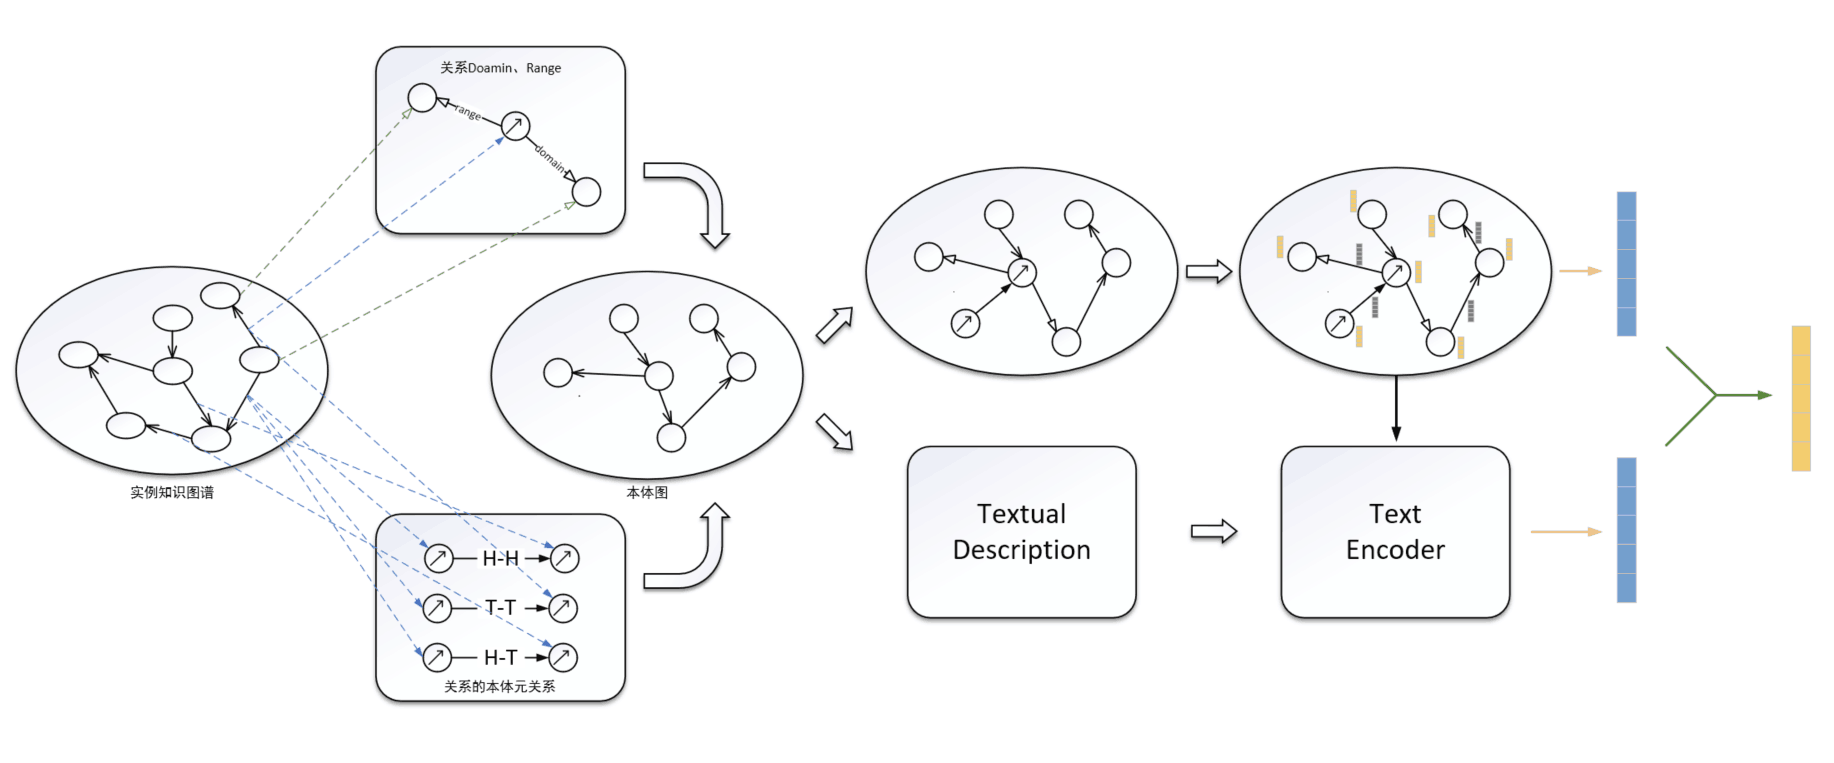
\includegraphics[width=1\textwidth]{new-3-1.png}
  \caption{本体嵌入整体框架}
  \label{fig:new-3-1}
\end{figure}

基于描述文本加强的本体嵌入框架主要包含两个部分,分别是关系本体构建和描述文本增强的本体表示。首先,作为本体嵌入的基础,本文了解到大多数引入本体信息的模型仅通过实体的类型和层次信息作为本体信息的体现,忽略了关系在本体中的体现。因此,本文首先对实例知识图谱中的关系进行处理,将关系的首尾实体抽象为实体类型,构建了关系的domain、range相关的本体三元组。考虑到知识图谱中关系的语义相关性,本文提出四种关系的位置元关系进一步对本体中的关系信息进行加强。而后在本体三元组的基础上学习对本体信息的嵌入。在通过传统KGE方法对本体三元组结构信息嵌入的基础上,本文又引入了本体节点的描述文本对本体嵌入的语义进行加强,获得了最终的本体向量表示。

\section{关系本体图构建}
结合本体的知识表示模型往往仅使用了类型、层次等信息,忽略了关系在本体中的重要体现。本节将介绍本文如何在现有的本体三元组基础上,对关系相关的本体三元组进行抽取。同时,根据关系的相对位置定义了四种关系的位置元关系,对本体中的关系信息进行补充和加强。

\subsection{关系本体三元组}
在RDF的设置下,知识图谱中的知识总是以三元组的形式出现,通过RDF的主语、谓语和宾语来描述事实。RDF通过类和属性描述个体之间的关系。这些类和属性由模式定义。RDF模式(RDF Schema,RDFS)提供了对类和属性的简单描述,一般用于对本体的简单定义。RDFS提供了最基本的对类和属性的描述元语:
\begin{itemize}
  \item rdfs:type:用于指定个体的类;
  \item rdfs:subClassOf:用于指定类的父类;
  \item rdfs:subPropertyOf:用于指定属性的父属性;
  \item rdfs:domain:用于指定属性的定义域;
  \item rdfs:range:用于指定属性的值域;
\end{itemize}

通过定义元语的方式来描述元数据之间的关系。同时,通过元语可以将知识分为两类:一类是数据层面的知识,如(Obama,type,Person)说明Obama是Person的一个实例;另一类是模式层面的知识,如(speaker,domain,Person)说明speaker属性的定义域是Person类。从简单意义上讲,数据层面的知识更多作用于实体,而模式层面的知识更多作用于关系。但当下将本体信息引入知识图谱嵌入的方法大多数仅采用数据层面的知识,忽略了模式层面知识对实例关系的知识补充。例如TransT\cite{ma2017transt}模型根据头尾实体的类型计算相似度作为知识图谱的先验知识改进三元组评分、JOIE\cite{hao2019universal}模型通过实体的本体类型信息将本体图和实例图进行跨视图的表示学习。这些模型主要通过本体的数据层面的知识,如实体类型对表示学习进行加强,更多偏向于实体的知识补充,忽略了对关系的补充。而跨域知识图谱中存在未见关系,本体中对关系模式的补充是非常必要的。

同样借助于实体的类型,本文通过对实例图谱中事实三元组的处理提取关系的本体三元组。如图\ref{fig:3-2}所示,对一个事实三元组(Obama,President\_of,America),其中头尾实体的类型(Obama,type,Person)和(America,type,Country),可知对于关系President\_of在本体中的定义域即头本体应该是类型Person,值域即尾本体,因此构建出相应的关系本体三元组(President\_of,domain,Person)和(President\_of,range,country)。
\begin{figure}[h]
  \centering
  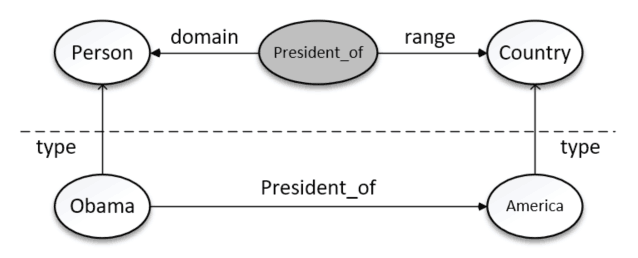
\includegraphics[width=0.8\textwidth]{new-3-2.png}
  \caption{关系本体三元组}
  \label{fig:3-2}
\end{figure}

但从源知识图谱直接抽取会产生大量的domain和range相关的关系本体三元组,其中包含了所有关系可能的值域和定义域。为了能够将抽取的关系的值域和定义域的本体三元组能够尽可能表示最普适的元信息,对于抽取所有的关系本体三元组,本文通过统计关系本体三元组在实例知识图谱中出现的频率,设置阈值对三元组进行筛选,以出现频率代表关系本体三元组的普适程度。除此之外,除了关系的domain和range的模式三元组,本文任务关系与关系之前存在相似性的关联,因此通过对关系描述文本的相似度匹配,计算关系与关系间的相似程度,本文还引入了关系与关系的联系和type本身的本体三元组中的isa、synonym关系共同设置为generalizations关系加入到本体三元组数据中。其中对关系描述文本的相似度匹配,本文采用word2vec进行文本嵌入和相似度计算。

\subsection{关系位置元关系}
上述关系本体三元组的抽取从值域和定义域的层面对本体中的关系信息进行了补充。除此之外,本文希望通过知识图谱中关系的语义相关性进一步对关系相关的语义信息进行捕捉。知识图谱中的实体具有隐含的语义相关性,例如北京和武汉在作为类型城市的实例具有相似的语义。而关系的语义相关性也非常常见,例如关系“/people/person/nationality”和“/people/ethnicity/languages\_spoken”具有很强的语义相关性,因为一个人说的语言很大程度上与他的国籍有关,在知识图谱上则可能直接表示为上述两个关系与同一个实体相关联。相反的,上述关系与语义差别很大的其他关系,如“/film/film/country”,则没有很强的语义相关性。并且这种语义相关性同关系的方向密切有关,如图\ref{fig:new-3-3}的“sister\_of”和通过e1节点连接的“has\_gender”,及通过e2节点连接的“sister\_gender”因为拓扑关系的不同,具备了完全不同的隐含信息。
\begin{figure}[h]
  \centering
  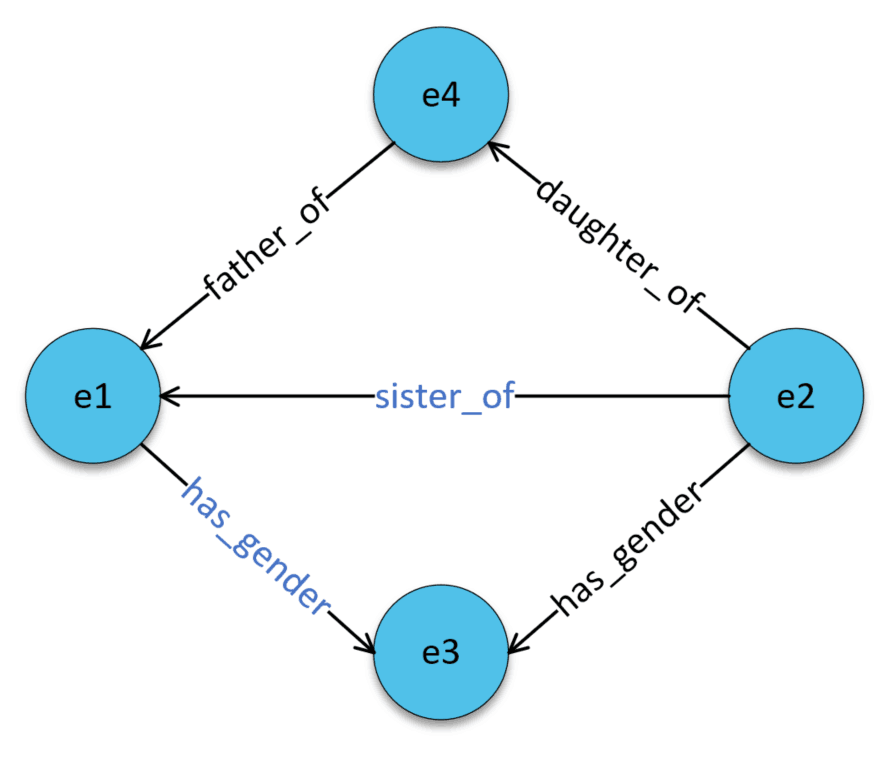
\includegraphics[width=0.5\textwidth]{new-3-3.png}
  \caption{关系位置实例}
  \label{fig:new-3-3}
\end{figure}

为了对两个关系之间的相关性进行建模,本文将关系与关系之间的拓扑关系建模为四种关系的位置元关系,分别为tail-head、head-tail、tail-tail、head-head。位置元关系的头结点和尾结点都代表了两个相邻关系的指向,比如(relation1,tail-head,relation2)代表同一个实体连接的两个相邻关系1和关系2,且关系1指向该实体而关系2则从该实体指向其他实体。对于在训练三元组中的两个关系,如果它们符合其中一种的相对未见关系,则提取一个位置元关系补充到本体三元组中。
\begin{figure}[h]
  \centering
  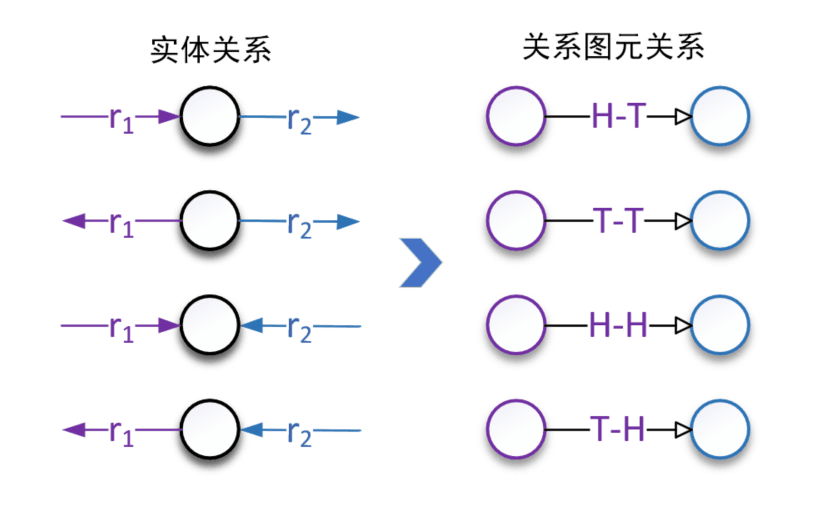
\includegraphics[width=0.7\textwidth]{3-4.png}
  \caption{实体关系与关系图元关系的映射}
  \label{fig:3-4}
\end{figure}

将位置元关系补充到本体三元组中后,本文希望通过传统的知识图谱嵌入方法对本体概念学习向量表示。但对位置元关系分析可知,“head-head”元关系自身、“tail-tail”元关系自身以及“head-tail”和“tail-head”元关系对都具有对称性。如图\ref{fig:new-3-3}中通过e1连接的“sister\_of”和“has\_gender”关系存在有(sister\_of,head-tail,has\_gender)与(has\_gender,tail-head,sister\_of),通过本文第2章对On2Vec模型的分析可知无法采用传统的KGE方法对有对称的元关系直接进行嵌入。因此,本文在补充位置元关系时仅保留了“head-tail”、“head-head”和“tail-tail”元关系,并且对“head-head”、“tail-tail”进行去重,避免了具有对称性位置元关系的存在。

通过对上述两种关系本体信息的补充,结合实体类型相关的本体三元组,本文在本体三元组中保留了domain、range、generalizations以及三个位置元关系总计6种元关系。本体三元组统计数据如下表\ref{tab:3-1}所示,最终构建出的本体图局部如图\ref{fig:new-3-5}所示。
% \begin{table}[h]
%   \caption{本体三元组统计信息}
%   \label{tab:3-1}
%   \centering
%   \resizebox{0.7\textwidth}{!}{%
%   \begin{tabular}{ccccc}
%   \hline
%   {\color[HTML]{333333} }         & {\color[HTML]{333333} 关系三元组数} & {\color[HTML]{333333} 元关系三元组数} & {\color[HTML]{333333} 其他三元组} & {\color[HTML]{333333} 总计}   \\ \hline
%   {\color[HTML]{333333} NELL\_Ext} & {\color[HTML]{333333} 1816}   & {\color[HTML]{333333} 2135}    & {\color[HTML]{333333} 332}   & {\color[HTML]{333333} 4326} \\
%   {\color[HTML]{333333} DB\_Ext}   & {\color[HTML]{333333} 1727}   & {\color[HTML]{333333} 1104}    & {\color[HTML]{333333} 464}   & {\color[HTML]{333333} 3295} \\ \hline
%   \end{tabular}%
%   }
%   \end{table}
\begin{table}[h]
  \caption{本体三元组统计信息}
  \label{tab:3-1}
  \centering
  \resizebox{0.7\textwidth}{!}{%
  \begin{tabular}{@{}ccccc@{}}
  \toprule
  {\color[HTML]{333333} }         & {\color[HTML]{333333} \textbf{关系三元组数}} & {\color[HTML]{333333} \textbf{元关系三元组数}} & {\color[HTML]{333333} \textbf{其他三元组}} & {\color[HTML]{333333} \textbf{总计}} \\ \midrule
  {\color[HTML]{333333} NELL\_Ext} & {\color[HTML]{333333} 1816}            & {\color[HTML]{333333} 2135}             & {\color[HTML]{333333} 332}            & {\color[HTML]{333333} 4326}        \\
  {\color[HTML]{333333} DB\_Ext}   & {\color[HTML]{333333} 1727}            & {\color[HTML]{333333} 1104}             & {\color[HTML]{333333} 464}            & {\color[HTML]{333333} 3295}        \\ \bottomrule
  \end{tabular}%
  }
  \end{table}
\begin{figure}[h]
  \centering
  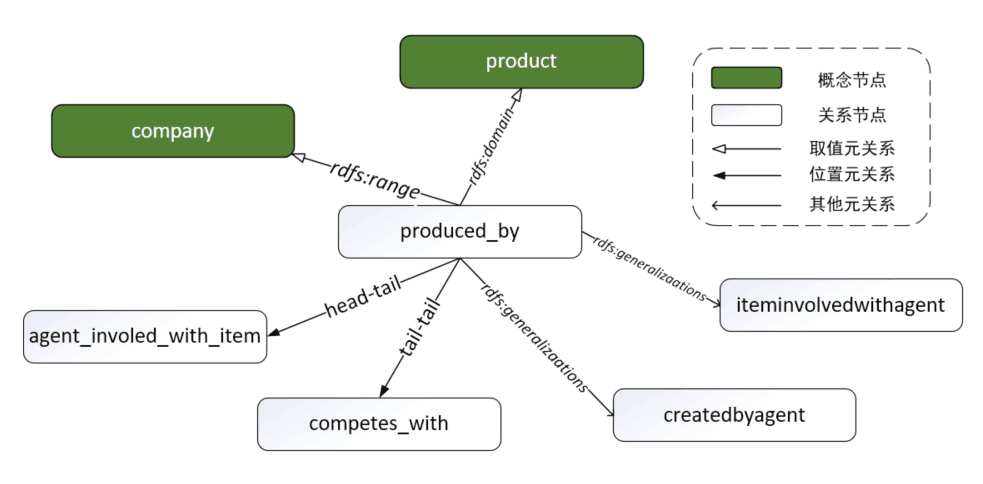
\includegraphics[width=0.9\textwidth]{new-3-5.png}
  \caption{关系本体图}
  \label{fig:new-3-5}
\end{figure}

\section{基于描述文本的本体表示增强}
为了将符号化的本体三元组用于后续对未见实体和未见关系的语义补充,需要将本体三元组转化为低纬向量表示。本节先从基础的本体三元组数据中学习到结构化的嵌入表示,然后从三元组的概念节点的描述信息中使用词嵌入学习到概念节点的描述文本嵌入。为了将描述文本的嵌入补充到本体信息的结构化中去,本文使用一个共享参数的线性层将结构化嵌入表示和描述文本嵌入表示映射到同一个表示空间中。在映射后的线性层中,参照TransE的评分思想,本文采用三个距离打分函数将映射后的两种嵌入表示联合更新,学习到兼顾结构信息和描述文本信息的嵌入表示。最后将两种表示拼接作为本体信息进行后续操作。基于描述文本的本体表示增强结构图\ref{fig:3-6}所示:
\begin{figure}[h]
  \centering
  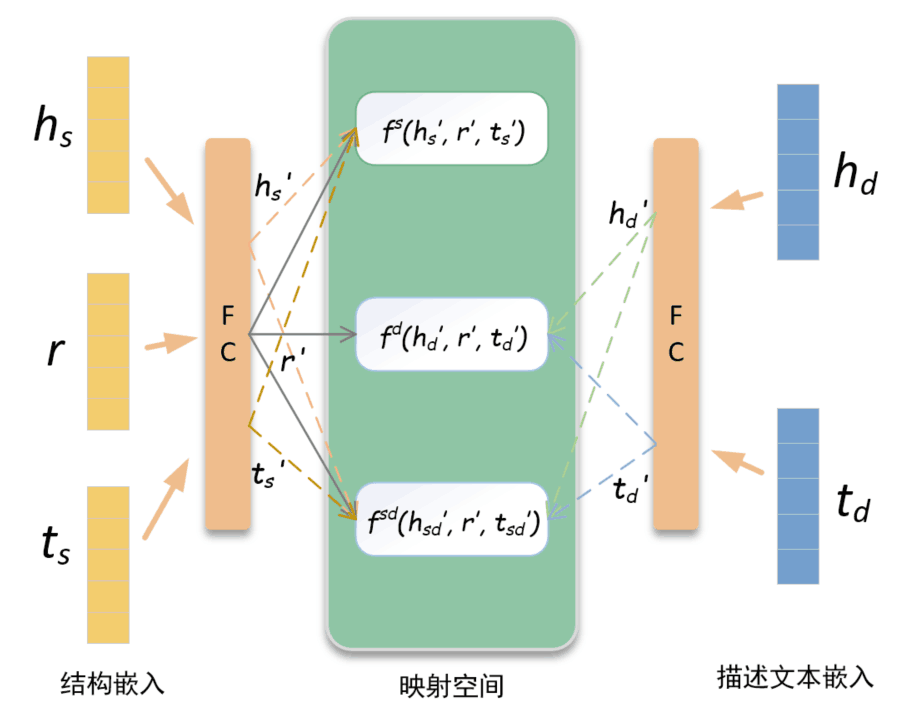
\includegraphics[width=0.9\textwidth]{3-2.png}
  \caption{本体嵌入架构}
  \label{fig:3-6}
\end{figure}

\subsection{本体结构信息嵌入}
对本体定义的结构化三元组进行嵌入的方法有很多种,因为在对本体三元组进行构建的时候本文已经尽可能减小了对称关系对嵌入效果的影响,因此可以通过多种传统的知识图谱嵌入方法学习本体表示。与传统的知识图谱嵌入表示类似,对于一个本体三元组\((c_{i},p,c_{j})\),本体语义信息编码的目的就是设计出一个打分函数\(f(c_{i},p,c_{j})\)作为编码模型的激活函数,本文采用RotatE对本体三元组进行编码。例如按照RotatE模型的设定,本体三元组的元关系属性是头尾两个实体节点的转移量,打分函数如公式\ref{eq:3-1}所示:
\begin{equation}
  f_{RotatE}(c_{i},p,c_{j}) = - \| \textbf{c}_{i} \circ \textbf{p} + \textbf{c}_{j}\|, \label{eq:3-1}
\end{equation}
其中\(\textbf{c}_{i}\),\(\textbf{p}\),\(\textbf{c}_{j}\)是一个本体三元组相应的概念编码和元关系编码,\(\circ\)指代了向量的旋转操作。同时为了提高所有本体三元组的嵌入效果,本文采用自对抗负抽样损失函数来计算损失更新模型,如公式\ref{eq:3-2}所示:
\begin{equation}
  \mathcal{L}_{\mathcal{O}} = \frac{1}{\mid \mathcal{T}_{\mathcal{O}}\mid} \sum_{(c_{i},p,c_{j}) \in \mathcal{T}_{\mathcal{O}}} [\gamma _{o} + f(c'_{i},p,c'_{j}) + f(c_{i},p,c_{j})], \label{eq:3-2}
\end{equation}
其中\(\gamma _{o}\)是控制正负样本得分的参数,同时\(c_{i}\),\(c_{j}\)是不存在于本体三元组中的负样本,为了生成这些负样本,本文在所有的本体概念中分别遮盖住已存在的本体三元组的头节点和尾结点,然后从所有本体节点中随机筛选出其他节点组成负样本。

\subsection{基于文本的本体嵌入}
除了结构化的本体三元组外,本体信息还有许多对本体进行详细描述的文本,如本体概念“companyceo”的描述文本“specifies that a particular CEO is the CEO of a particular company”。这些描述文本可以为本体信息提取提供额外的语义信息,因此本文通过使用文本描述来加强对本体三元组的语义嵌入。然而,描述文本的建模与一般的三元组建模因模型的差异而无法直接融合。因此对于给定的本体三元组\((c_{i},p,c_{j})\),本文首先获得了三元组的结构嵌入\(h_{s}/r/t_{s} \in \mathbb{R}^{d_{1}}\)和每个本体节点描述文本的向量表示\(h_{d}/t_{d} \in \mathbb{R}^{d_{2}}\),表示文本描述信息。为了融合这两个不同层面的嵌入,本文引入了一个全连接层,将两个不同的嵌入同时映射到同一表示维度上。映射后的结构嵌入和文本嵌入分别表示为\(h_{s}^{'}\)和\(h_{d}^{'}\),在统一表示空间中,使用TransE对三元组结构的嵌入进行打分,打分函数如公式\ref{eq:3-3}所示:
\begin{equation}
  f^{s} = -  \parallel h'_{s} + r' - t'_{s}  \parallel, \label{eq:3-3}
\end{equation}

对描述文本的嵌入进行打分,打分函数如公式\ref{eq:3-4}所示:
\begin{equation}
  f^{d} = -  \parallel h'_{d} + r' - t'_{d}  \parallel, \label{eq:3-4}
\end{equation}

同时为了为了使这两种类型的表示相互兼容和互补,本文遵循DKRL模型的设定来定义交叉和相加得分函数,打分函数如公式\ref{eq:3-5}所示:
\begin{equation}
  f^{sd} = -  \parallel h'_{s} + r' - t'_{d}  \parallel -  \parallel h'_{d} + r' - t'_{s}  \parallel, \label{eq:3-5}
\end{equation}

所有的四个得分函数综合可以保证两个层面的嵌入表示可以在相同空间里进行学习和更新,最后本体嵌入的得分函数如公式\ref{eq:3-6}所示:
\begin{equation}
  f'(c_{i},p,c_{j}) = f^{s} + f^{d} +f^{sd}, \label{eq:3-6}
\end{equation}

因此在本体嵌入的损失函数也响应的转化为:
\begin{equation}
  \mathcal{L}_{\mathcal{O}}^{ont} = \frac{1}{\mid \mathcal{T}_{\mathcal{O}}\mid} \sum_{(c_{i},p,c_{j}) \in \mathcal{T}_{\mathcal{O}}} [\gamma _{o} + f'(c'_{i},p,c'_{j}) + f'(c_{i},p,c_{j})], \label{eq:3-7}
\end{equation}

经过训练后每个本体节点都有两个层面的嵌入:三元组结构嵌入和描述文本嵌入。本文将这两种映射后的嵌入进行拼接作为本体节点的最终的向量表示。上述的描述文本的向量表示,本文采用了词袋模型进行生成。

\section{本章小结}
本章通过对本体三元组的关系部分构建,强调了关系在本体信息中的体现。尤其是在处理跨域知识图谱中存在的新的关系,本体中的信息能够对关系表示进行有效的语义补充。通过本体三元组的结构信息和本体的描述文本信息,能够学习到好的本体嵌入,为下一章未见关系的建模提供了良好的先验知识。
\chapter{基于元学习本体增强的跨域知识表示学习模型}
跨域知识图谱的知识表示学习关键在于如何对目标域知识图谱中的未见关系和未见实体进行嵌入,以解决零样本问题。受到元学习算法思想的启发,本文通过设置多个训练任务,在任务中模拟存在新的实体和新的关系的跨域场景,并基于训练任务进行模型训练,使得模型能够学习到对未见实体和未见关系的嵌入能力。在每一个训练任务上,模型通过对关系的拓扑信息和本体信息进行学习获得对未见关系的嵌入表示,通过对未见实体邻接的关系信息聚合获得未见实体的嵌入表示。为充分利用到已知关系和已知实体的特征信息,本文采用CompGCN在实例知识图谱上对所有实体和关系的初始化嵌入再进行一次更新,获得所有实体和关系最终的向量表示。最后通过多个KGE方法计算损失并进行模型优化。该模型的主要创新点如下:1)关系和实体的表示能够同时学习到事实三元组结构上的拓扑信息和本体层面上的语义信息。2)能够通过元学习的训练流程模拟出目标问题的学习任务并对模型参数进行更新。3)能够同时对测试集中未见的关系和未见的实体嵌入编码。

\section{模型整体架构}
\begin{figure}[h]
  \centering
  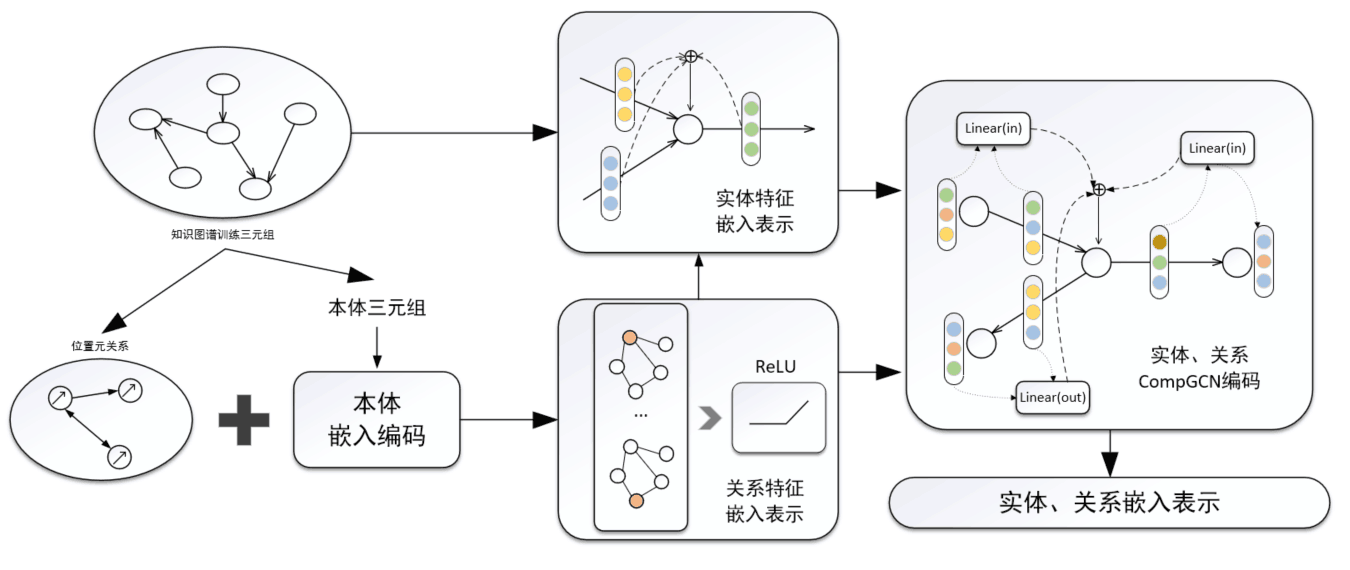
\includegraphics[width=1\textwidth]{3-1.png}
  \caption{模型架构图}
  \label{fig:3-1}
\end{figure}

本文提出的模型整体结构如图\ref{fig:3-1}所示,包含三个主要的部分:未见关系嵌入、未见实体嵌入以及元学习训练设定。对于跨域知识图谱上未见关系的特征提取,本文首先根据实例图谱中关系的相对位置构建了关系位置图,其中节点为实例图谱中的关系。本体信息和关系位置图结合后,通过两层GCN对关系的语义信息和结构信息进行更新和学习,获得关系特征的嵌入表示。对于未见实体的表示学习,本文对未见实体的邻接关系进行聚合,并使用关系方向特定的调整矩阵,提取所有关系的特征,以获得实体特征的嵌入表示。为了利用实例图谱中的已知关系和已知实体,本文在实例图谱上采用两层CompGCN聚合所有实体和关系及其邻域特征,并对它们的嵌入表示进行更新。模型修改了CompGCN的输出层,使得关系和实体的维度不要求一致,从而可以采用多种KGE模型作为打分函数来计算损失,以对模型进行调优。而为了能够让模型在训练过程中获得对目标域知识图谱未见实体和关系表示学习的能力,本文设置了多个训练任务对跨域场景进行模拟,在训练任务上获得最优参数,并将训练的参数用于目标域的图谱嵌入上。

对于训练集中可见的关系和实体,本文采用了传统的知识图谱表示学习的学习流程,即分别设置关系特征矩阵和实体特征矩阵,在初始化阶段对这两个矩阵按照各自目标维度随机向量初始化。在模型训练过程中通过TransE等打分函数对嵌入结果打分后进行更新,可以得到可见部分的特征嵌入。

\section{未见关系的特征嵌入}
\subsection{关系位置图构建}
为了能够对目标域知识图谱中的未见关系进行有效的特征学习,由于在源知识图谱中不存在相关的事实三元组可以提供知识,必须要从其他层面获取到对未见关系编码有效的语义信息。本文在第三章中为本体添加了关系的本体三元组,学习到了关系在本体层面的语义信息。同样,基于第三章的关系位置元关系的设定,源域知识图谱中所有的关系可以在关系位置图中进行表示,关系与关系之间通过已定义的四种关系位置元关系(tail-head,tail-tail,head-head,head-tail)进行连接。在关系位置图中,关系与关系间的位置联系可以作为关系的一种拓扑特征信息。这些结构性的信息会减少对具体实体和关系的依赖,在对关系特征进行学习的时候,通过聚合相连其他关系的信息来对关系进行特征表示,能够作用在未见的关系上。
\begin{figure}[h]
  \centering
  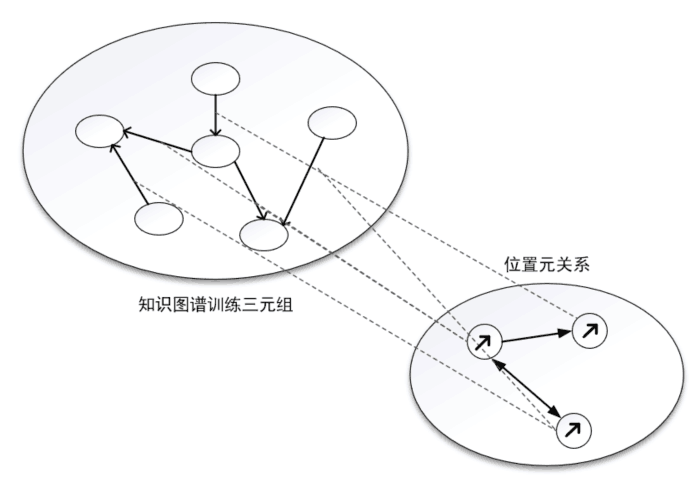
\includegraphics[width=0.5\textwidth]{3-3.png}
  \caption{实例图构建关系图}
  \label{fig:3-3}
\end{figure}

与第三章抽取关系的位置元关系不同,在位置关系图中,本节没有对图中具有对称性的位置元关系进行筛选和去除。为了防止对图中对称的元关系重复的进行信息传递,在对关系节点进行特征聚合时,本节仅考虑每个关系节点的入向关系,以此避免了位置元关系的对称性的影响。

对于输入的实体三元组,可以将原始的图结构转变为关系相关图,如图\ref{fig:3-3}所示。同时在构建图的过程中没有使用到任何额外的实体属性或关系属性,可以作用到任何未见或已知的关系上。关系相关图中的节点代表原始三元组中的关系,边表示在原始三元组任意两个关系对应的元关系。

\subsection{关系相关性系数聚合编码}
在关系位置图中,结点为原三元组中的关系,可以通过聚合关系结点的其他相邻关系结点的特征作为该关系的特征。为了能够将本体的嵌入作为对关系嵌入的语义补充,在构建好的关系位置图上,本文通过关系节点到本体概念的映射获取到各关系节点的初始化特征表示。然后通过多层图卷积网络聚合邻接节点的特征来对关系节点的特征学习,对于节点的更新公式如公式\ref{eq:4-4}所示:
\begin{equation}
  h_{v}^{l+1}= f\left( \sum_{u \in \mathcal{N}(v)} \frac{1}{c_{u}} h_{u}^{l} W^{l}\right) \label{eq:4-4}
\end{equation}
其中\(h_{u}^{l}\)是关系节点\(v\)相邻节点的特征。每层图卷积会有两步的操作,首先左乘归一化因子(如节点度的倒数)聚合邻接点的特征,然后右乘一个可学习的线性转换矩阵\(W\),再使用一个非线性的激活函数来获取本层的特征输出。

为了在聚合关系本体信息和拓扑信息时区分不同元关系的重要性,本文在对不同元关系连接的关系特征进行聚合时设置一个可学习的权重参数,根据任务的表现来学习不同元关系对应的重要程度,计算公式转化如公式\ref{eq:4-5}所示:
\begin{equation}
  h_{v}^{l+1} = f\left( \sum_{(u,r) \in \mathcal{N}(v)} \frac{1}{c_{u,r}} h_{u}^{l} W_{ dir(r) }^{l}\right) \label{eq:4-5}
\end{equation}
其中\(W_{dir(r)}\)是两个关系节点相连的元关系类型相对应的参数,根据本文设定的四种不同的元关系,该系数由四个不同的参数控制,如公式\ref{eq:4-6}所示:
\begin{equation}
  W_{dir(r)} = \left\{ \begin{array}{rcl}
    &W_{t-h}  \mbox{,} &\quad r \in R_{tail-head} \\
    &W_{h-t}  \mbox{,} &\quad  r \in R_{head-tail} \\
    &W_{t-t}  \mbox{,} &\quad  r \in R_{tail-tail} \\
    &W_{h-h}  \mbox{,} &\quad  r \in R_{head-head} \\
    \end{array}\right\} \label{eq:4-6}
\end{equation}

\section{未见实体的特征嵌入}
\subsection{基于关系聚合的实体表示}
传统的知识表示学习通过对知识图谱三元组的结构信息学习,能够使表示向量尽可能贴近事实。但在目标域知识图谱中存在未见实体的情况下,由于缺乏事实三元组的支撑,传统的KGE方法无法学习到未见实体的特征信息。

为了解决上述问题,本文借鉴人类对未见实体的推理过程来对未见实体进行编码。如图\ref{fig:3-5}所示,传统的KGE方法能够通过对事实三元组的学习,对已知的Tom节点进行有效的学习。对于存在未见实体的目标域知识图谱,常人虽然无法获得节点X、Y、Z、A的具体内容,但是通过对左右两个图谱的推理可知,X具有和Tom类似的邻域结构信息,如student\_of、advisor\_of及lives\_in等,因此,节点X应该是一个类似于Tom的一个学生类型的节点。这些结构性的信息可以帮助人去理解一个新的实体,同时这些实体的邻域结构信息与实体本身具体信息是无关且通用的。
\begin{figure}[h]
  \centering
  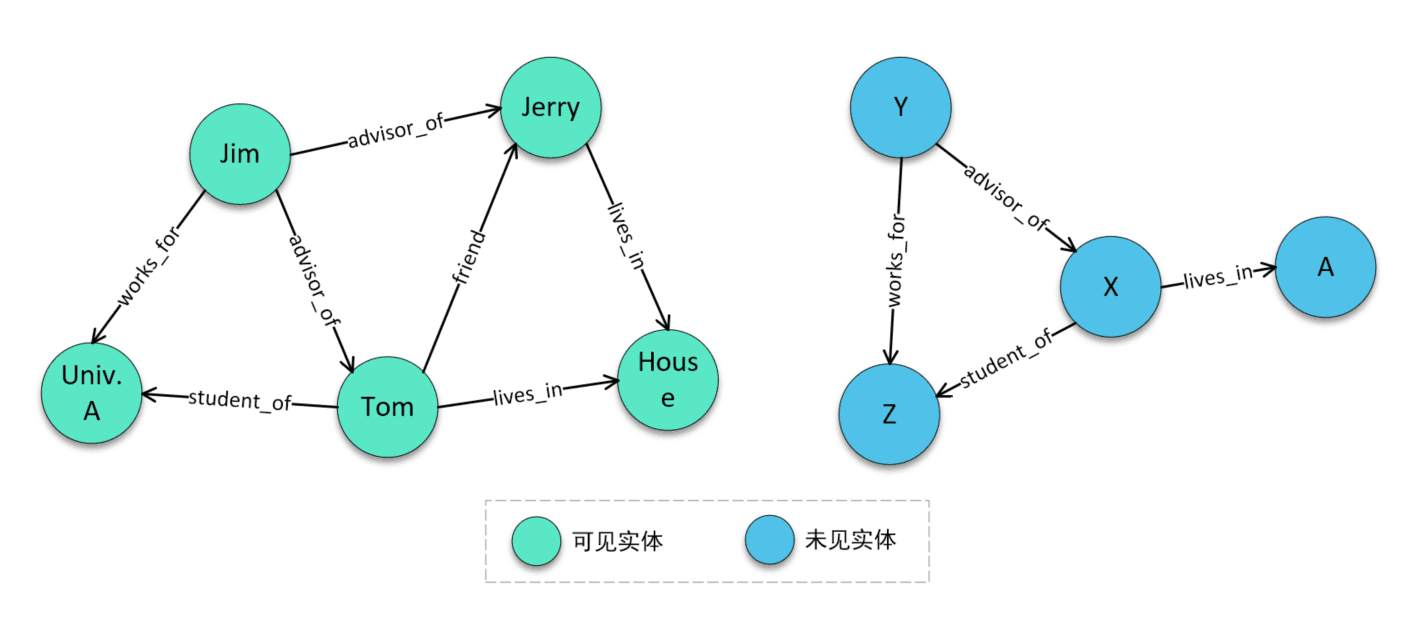
\includegraphics[width=0.8\textwidth]{3-5.png}
  \caption{未见实体的关系特征}
  \label{fig:3-5}
\end{figure}

本节通过模拟人类对新实体的推理过程,对实体邻域的结构信息进行建模来获得实体的特征编码。实体邻域结构信息最直接的体现便是与实体直接联系的各个关系,因此本节通过使用实体相关的关系信息获得未见实体的嵌入。同时考虑到实体关系的方向性,本文通过公式\ref{eq:4-7}来进行实体关系的聚合:
\begin{equation}
  \textbf{h}_{e} = \frac{1}{|\mathcal{I}(e)| + |\mathcal{O}(e)|} \left(
    \sum_{r\in \mathcal{I}(e)}\textbf{W}_{in}^{ent} \textbf{h}_{r} +
    \sum_{r\in \mathcal{O}(e)}\textbf{W}_{out}^{ent} \textbf{h}_{r}
    \right) \label{eq:4-7}
\end{equation}
其中\(\mathcal{I}(e)\)是实体e所有连接关系中指向实体e的集合,\(\mathcal{O}(e)\)是实体e所有连接关系中由实体e出发指向其他实体的关系集合,\(\textbf{W}_{in}^{ent}\)和\(\textbf{W}_{out}^{ent}\)分别是用于在聚合实体邻接关系中入关系和出关系是对关系嵌入的权重矩阵。

然而,通过对实体的关系特征进行聚合只能获得实体的初始化嵌入,因为实体的邻域结构只传递类型级别的信息,而不是实例级别的。例如,对于节点X,我们只能推断出该节点是一个类似Tom的学生类型节点,但无法得知节点X具体是谁。为了解决这个问题,本文在下一节引入了基于GNN的实体关系联合嵌入模块,根据实体的多跳邻域结构调制每个实体和关系的初始化嵌入。

\subsection{基于GNN的实体关系联合嵌入}
在上述两个章节中,本文通过关系的本体信息和拓扑信息学习到了未见关系的初始化嵌入,通过实体的邻域结构信息的聚合学习到了未见实体的初始化嵌入。但是这些初始化的嵌入仅传递了部分信息,如实体偏向于类型的初始化嵌入,没有充分利用到已知实体和已知关系的信息。因此,本文在实例知识图谱上,通过借鉴CompGCN的模型结构,设计了一个能够同时对实体和关系进行邻域信息聚合的模块。该模块通过对每一个实体和关系聚合多跳邻域结构信息,充分利用到所有已知关系和已知实体的信息,学习到未见实体和未见关系更充分的语义表示。

该层GNN网络虽然以CompGCN模型为基础,但是CompGCN原模型在对关系和实体进行聚合操作的时候采用了TransE、HoLE和DistMul模型的评分函数,限制了关系和实体的维度必须一致。为了使得该GNN网络能够输出维度不同的实体和关系的编码,本文借鉴MaKEr\cite{chen2022meta}模型的设置,将CompGCN模型原有的实体关系聚合器修改为一个线性转化层,可以让模型更好适应以多种传统KGE方法如RotatE来作为解码器进行下游任务。各层的实体嵌入更新公式如公式\ref{eq:4-8}所示:
\begin{equation}
\textbf{h}_{e}^{l+1} = f \left(
\frac{\sum_{(r,e)\in \mathcal{N}(e)}\textbf{W}_{dir(r)}^{l} [\textbf{h}_{r}^{l} ; \textbf{h}_{e}^{l}]}{|\mathcal{N}(e)|} + \textbf{W}_{self}^{l}\textbf{h}_{e}^{l}
\right) \label{eq:4-8}
\end{equation}
其中\(\mathcal{N}(e)\)是实体e的所有相连的关系集合,\(\textbf{W}_{dir(r)}^{l}\)是对集合中关系不同方向特定的权重参数,入方向和出方向时分别记为\(\textbf{W}_{in}^{l}\)和\(\textbf{W}_{out}^{l}\),\([;]\)指代两个向量的连接操作。\(\textbf{W}_{self}^{l}\)是针对实体e本身特征自循环更新的模型学习参数,\(f\)指代模型GNN模型的激活函数。同时,关系也在该层网络中也进行了更新操作,如公式\ref{eq:4-9}所示:
\begin{equation}
\textbf{h}_{r}^{l+1} = \textbf{W}_{rel}^{l}\textbf{h}_{r}^{l} \label{eq:4-9}
\end{equation}

经过两层GNN网络,关系嵌入和实体嵌入得到了更新,该模块输出的是该训练任务下所有实体和关系的知识表示嵌入,用于本次任务的损失计算及模型参数更新。

\section{基于元学习的训练任务设定}
为了能够对知识图谱中的未见关系和未见实体进行表示学习,借鉴于元学习“learning to learn”的思想,本文设置了训练元任务和测试元任务。训练元任务用于训练元学习算法,即在训练过程中让算法从元任务中获取经验并调整参数,以便于在测试任务中能够快速地适应。测试元任务则是在训练完成后用于测试元学习算法性能。不同于元学习一般划分多个不同元任务的设定,本文采用单任务设定,即训练元任务和测试元任务均视为单一的任务。单任务设定可以使得元学习算法更加适应目标任务,并提高模型的泛化能力。同时,模型可以更加专注于学习适应固定任务的策略,还可以减少模型的计算和存储成本,并使得模型更加容易调整和解释。

本文从训练集中抽取了一系列包含未见实体和关系的训练任务来模拟跨域环境,并在该训练环境中对模型进行训练。每个训练任务\(T^{i} = (\mathcal{E}^{i}, \mathcal{R}^{i}, \mathcal{T}^{i}_{sup},\mathcal{T}^{i}_{que})\)包含训练实体集、关系集、support训练三元组集以及query测试三元组集。为了模拟未见的组件,将部分实体和关系标记为未见,每个训练任务被重新定义为如\ref{eq:4-1}所示:
\begin{equation}
  T^{i} = (\mathcal{E}^{i} = (\hat{\mathcal{E}}^{i},\tilde{\mathcal{E}}^{i}), \mathcal{R}^{i} = (\hat{\mathcal{R}}^{i} ,\tilde{\mathcal{R}}^{i}   ), \mathcal{T}^{i}_{sup},\mathcal{T}^{i}_{que})  \label{eq:4-1}
\end{equation}
其中\(\hat{\mathcal{E}}^{i} \in \mathcal{E}^{train}\)指代实体集中的可见实体而\(\tilde{\mathcal{E}}^{i} \notin \mathcal{E}^{train}\)指代未见的实体;\(\hat{\mathcal{R}}^{i} \in \mathcal{R}^{train}\)指代关系集中的可见关系\(\tilde{\mathcal{R}}^{i} \notin \mathcal{R}^{train}\)指代未见的关系。对训练集中三元组抽取训练任务和测试任务的流程如算法\ref{alg:task}所示:
\begin{algorithm}
  \KwData{读取所有三元组,构建大图\(\mathcal{G}_{train}\)}
  \For{i < num\_subgraph}{
    选取num\_root个根节点\\
    \While{子图节点 < 50}{
      从根节点随机游走num\_step步,构建子图\(\mathcal{G}_{i}\)
    }
    从子图三元组中抽取10\%作为query三元组\\
    对query三元组中的关系和实体随机标记为未见\\
    构建support三元组中的实体和关系联系矩阵,构建关系位置图\\
    将support三元组、query三元组、关系位置图存储
  }
  \caption{任务子图构建流程}\label{alg:task}
\end{algorithm}

所有训练的总目标是:在每个任务的support集上对未见实体和关系的学习能力训练,使得在query集上的评估得分最高,计算函数如公式\ref{eq:4-2}所示:
\begin{equation}
  \max\limits_{ \theta } \mathbb{E} _ { T ^ { i } \sim p ( T ) } \left[ \sum\limits_{ ( h , r , t ) \in \mathcal{T} _ { \text { que } } ^ { i } } \frac { 1 } { | \mathcal{T} _ { \text { que } } ^ { i } | } \mathcal{M} ( h , r , t | \mathcal{T} _ { \text { sup } } ^ { i } ) \right] \label{eq:4-2}
\end{equation}
其中\(\mathcal{M}\)通过在support集上学习到实体和关系的嵌入表示,并在query集上对三元组计算得分。本文采用自对抗负抽样损失函数来对计算损失更新模型,如公式\ref{eq:4-3}所示:
\begin{equation}
  \begin{aligned}
    \mathcal{L}(T^{i}) = &\frac{1}{|\mathcal{T}^{i}_{que}|} \sum\limits_{(h,r,t)\in\mathcal{T}^{i}_{que}}-log\sigma(\gamma + s(h,r,t)) \\
    &-\sum\limits_{i=1}^{n}p(h'_{i},r,t'_{i})log\sigma(-\gamma - s(h,r,t)) \label{eq:4-3}
  \end{aligned}
\end{equation}
n指代负采样的数量,\(p(h'_{i},r,t'_{i})\)指代负采样的权重系数,\(s(h,r,t)\)是用于计算嵌入向量在query三元组上的得分函数。

\section{基于链接预测任务的模型实现}
知识图谱的知识表示学习通过学习实体和关系的向量表示,来捕捉隐含的语义关系和规律。跨域知识图谱的知识表示学习在传统知识表示学习的基础上,能够学习到目标域知识图谱上新的实体和关系的特征表示。为了验证知识表示学习的有效性,本文结合下游链接预测任务对提出的知识表示学习方法进行评判。

链接预测任务通常涉及知识图谱中实体对之间的关系推理。该任务基于现有事实来推断出未知的三元组,以帮助补全知识图谱中的缺失信息、推断未知实体之间的关系及预测新实体属性等。链接预测任务可分为头实体预测和尾实体预测两种类型。为了评估模型在链接预测方面的能力,常用的指标有MRR和Hits@k等。其中MRR被定义为测试数据集中每个三元组的预测排序的平均排名的倒数,而Hits@k则是指在测试数据集中每个三元组的预测概率排名中前k名的正确率,即命中率。这些指标可以帮助确定预测结果的准确性和可靠性,同时有助于对不同模型进行比较和评估。

本文在训练任务的support上学习到实体和关系的嵌入,并在query集上进行损失计算。在进行每次任务损失的过程中,通过正负样本的联合计算出损失,并以此进行梯度下降求解。负样本损失计算公式如公式\ref{eq:4-10}所示:
\begin{equation}
  \mathcal{L}_{neg} = \sum_{i = 1}^{n} \left( softmax(W[s_{tail};s_{head}])log \sigma (- [s_{tail};s_{head}]) \right) \label{eq:4-10}
\end{equation}
其中\(s_{tail}\)和\(s_{head}\)是对一个测试三元组对应的尾结点负采样得分和头结点负采样得分,n代表负采样的数量,\([;]\)操作将正负样本的得分矩阵进行简单的连接操作,\(W\)是对得分进行微调的权重参数,本文默认设置为1。正负样本的得分求得算术平均即为该测试三元组的单个损失。

对于模型的训练流程,本文按照元学习单任务训练方法进行,每个任务的目标都是使该任务下的连接预测效果最优,单个任务的训练流程包含有5步:

\begin{enumerate}[label=\arabic*)]
  \item 初始化模型参数,主要包含了训练数据集中可见实体和关系的嵌入初始化、元关系的权重参数以及两个不同阶段的GCN层和CompGCN层的传递参数。
  \item 获得任务的支持集和查询集,主要从原训练集中抽取单个任务的子图,并划分为支持集和查询集,同时对关系和节点的标签进行设置以模拟出未见组件。
  \item 单次任务训练获得实体关系的嵌入,通过KGE模型计算查询集损失,利用梯度下降求解。
  \item 更新模型参数,重复下一个任务的训练直至效果不再更优。
  \item 对测试集进行模型测试,输出任务得分。
\end{enumerate}

\section{本章小结}
本章从本文模型的总体架构开始,详细介绍了模型的各个组成部分,包括主要的未见关系嵌入、未见实体嵌入以及基于元学习的训练任务设定和基于链接预测任务的模型实现的说明。对未见关系嵌入,说明了本文模型如何对关系的拓扑结构进行提取以及如何通过图卷积层对关系的本体信息和拓扑信息进行联合学习,从而获得未见关系的有效表示;对未见实体嵌入,通过未见实体的邻接关系的特征聚合,并且在实例知识图谱上通过GNN来聚合其他关系和实体信息,完成最后的实体和关系的特征更新。之后的章节中将对本文模型在测试数据集上进行充分的实验,检验本文模型的有效性。
% \chapter{基于元学习本体增强的跨设备知识图谱表示模型}
本章将详细介绍提出的基于元学习本体增强的跨领域知识图谱表示学习模型的各个部分。本章首节对模型要解决的问题和测试的任务作出符号上的定义和解释;然后将介绍本文设计模型的整体框架以及对框架组成进行大概的描述;然后详细说明该知识表示模型的三个主要组成模块:关系编码模块、实体编码模块以及模型整体元学习训练设定与训练流程。此外对于训练集中可见的关系和实体,本文采用了传统的知识图谱表示学习的学习流程,即分别设置关系特征矩阵和实体特征矩阵,在初始化阶段对这两个矩阵按照各自目标维度随机赋值,在模型训练过程中通过TransE等打分函数对特征进行打分后进行更新,可以得到可见组件的特征嵌入。本章主要讲解本未见的组件进行编码的过程。该模型的主要创新点如下:(1)关系和实体的表示能够同时学习到实体三元组结构上的拓扑信息和本体层面上的语义信息。(2)能够通过元学习的训练流程模拟出目标问题的学习任务对模型参数进行更新。(3)能够同时对测试集中未见的关系和未见的实体嵌入编码。
\section{问题定义}
一个单独的知识图谱通常定义为\(\mathcal{G} = (\mathcal{E},\mathcal{R},\mathcal{T})\),其中\(\mathcal{E}\)指代所有图谱实体的集合,\(\mathcal{R}\)指代图谱所有关系的集合而\(\mathcal{T}\)指代所有的实体三元组,而且对于三元组集合\(\mathcal{T}=\{(h,r,t) \subseteq \mathcal{E} \times \mathcal{R} \times \mathcal{E}\}\),即所有的三元组的头尾实体和关系均来自于实体集\(\mathcal{E}\)和关系集\(\mathcal{R}\)中。对于知识图谱上的链接预测任务,则是给定一个三元组的头结点和关系\((h,r,?)\)或者尾结点和关系\((?,r,t)\)来预测缺失的实体节点\(e \in \mathcal{E}\),使得该缺失的实体节点能构成一个事实三元组\((h,r,t)\)来完成对原始知识图谱的知识补全。为了评估表示学习模型在链接预测任务上的效果,通常会设置两组三元组数据,一组训练三元组\(\mathcal{T}_{support}\)用于对表示学习模型的参数进行学习,另一组测试三元组\(\mathcal{T}_{query}\)包含了训练集中不存在的知识图谱的其他隐藏的事实三元组用于对模型的学习效果进行测试。例如对一个尾结点的预测任务,给定在测试三元组中的一个事实\((h,r,t) \in \mathcal{T}_{query}\),通过模型计算所有可能预测三元组\(\{(h,r,e) | e \in \mathcal{E}, (h,r,e) \notin \mathcal{T}_{support} \cup \mathcal{T}_{query}\}\),如果在所有预测三元组中\((h,r,t)\)的得分越高则说明该表示模型的效果越好。

而在跨设备的训练场景下,本文对传统的知识图谱链接预测任务的定义进行了场景适配。现给定一个基础的训练知识图谱\(\mathcal{G}^{train} = (\mathcal{E}^{train},\mathcal{R}^{train},\mathcal{T}^{train})\),训练的目标是在训练知识图谱上进行模型参数的学习,从而能够将该模型应用在包含未见组件的新兴测试知识图谱上,即\(\mathcal{G}^{test} = (\mathcal{E}^{test},\mathcal{R}^{test},\mathcal{T}^{test}_{support},\mathcal{T}^{test}_{query})\),其中的实体集和关系集遵循\((\mathcal{E}^{train} \neq \mathcal{E}^{test},\mathcal{E}^{train} \cap \mathcal{E}^{test} \neq \emptyset)\)及\((\mathcal{R}^{train} \neq \mathcal{R}^{test},\mathcal{R}^{train} \cap \mathcal{R}^{test} \neq \emptyset)\)。其中只用于标记测试集中实体与关系的结构,不用于对模型的训练。而且在跨设备的设定下,测试数据集和训练数据集无法进行数据合并。
\section{模型整体架构}
\begin{figure}[h]
  \centering
  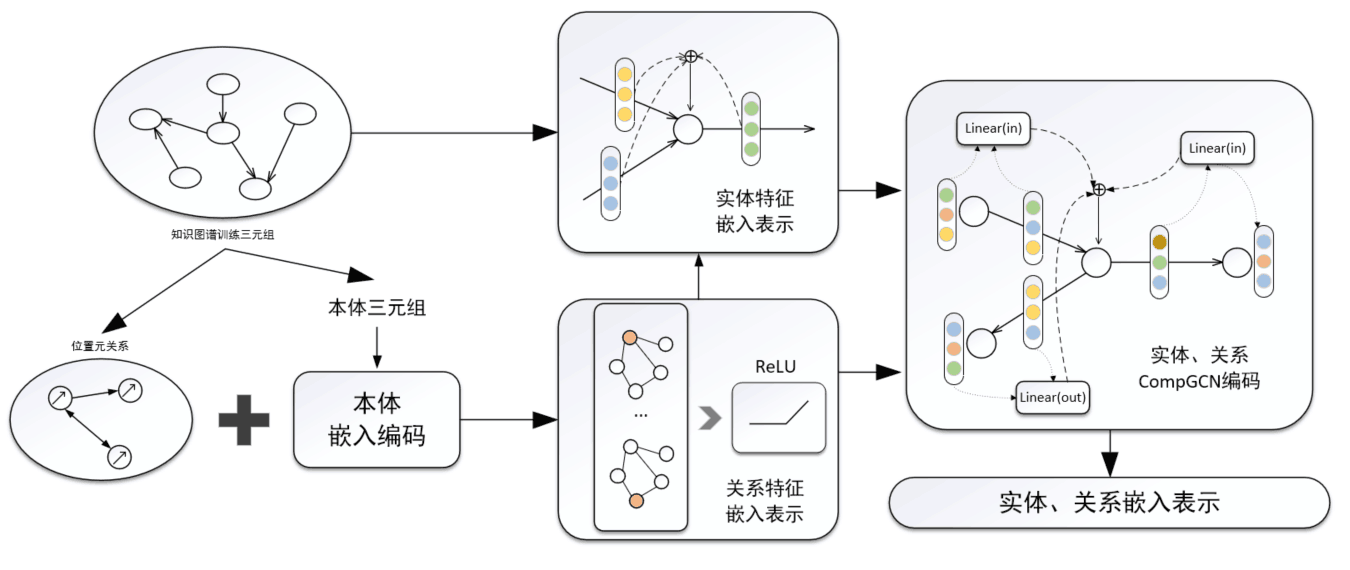
\includegraphics[width=1\textwidth]{3-1.png}
  \caption{模型架构图}
  \label{fig:3-1}
\end{figure}
本文提出的模型整体结构图如图\ref{fig:3-1}所示,总体包含三个大的模块:关系编码模块、实体编码模块、实体关系联合嵌入模块。

为了对关系的特征进行提取,本文模型首先根据实例图谱中的关系的相对位置结构构建出关系位置图,该图中的节点为实例图谱中的关系。然后基于图谱的本体三元组信息对本体的关系及概念节点进行嵌入,为了补充本体的信息,同时采用概念节点的描述文本对本体嵌入进行加强;然后将本体信息和关系位置图进行结合,通过两层GCN模型对关系的语义信息和结构信息进行更新和学习,获得关系特征的嵌入表示。对实体的表示上,通过聚合实体邻接关系,通过学习关系方向调整矩阵的参数来对所有关系的特征进行提取获得实体特征的嵌入表示。最后为了加强实体与关系的联系,本文模型在实例图谱上进行两层CompGCN的特征提取获得了最终的实体和关系的嵌入,同时修改了CompGCN的输出层使得关系和实体的维度不要求一致,从而可以通过多种KGE模型作为打分函数计算损失函数对模型调优。

其中对本体嵌入的过程中,本文首先从基础的三元组数据中学习到结构化的嵌入表示,然后从三元组的概念节点的描述信息中使用词嵌入学习到概念节点的描述文本嵌入,为了将描述文本的嵌入补充到本体信息的结构化中去,本文使用一个共享参数的线性层将结构化嵌入表示和描述文本嵌入表示映射到同一个表示空间中。在映射后的线性层中,参照TransE的评分思想,本文采用三个距离打分函数将映射后的两种嵌入表示联合更新,学习到兼顾结构信息和描述文本信息的嵌入表示。最后将两种表示拼接作为本体信息进行后续操作。本体嵌入整体结构图如下:
\begin{figure}[h]
  \centering
  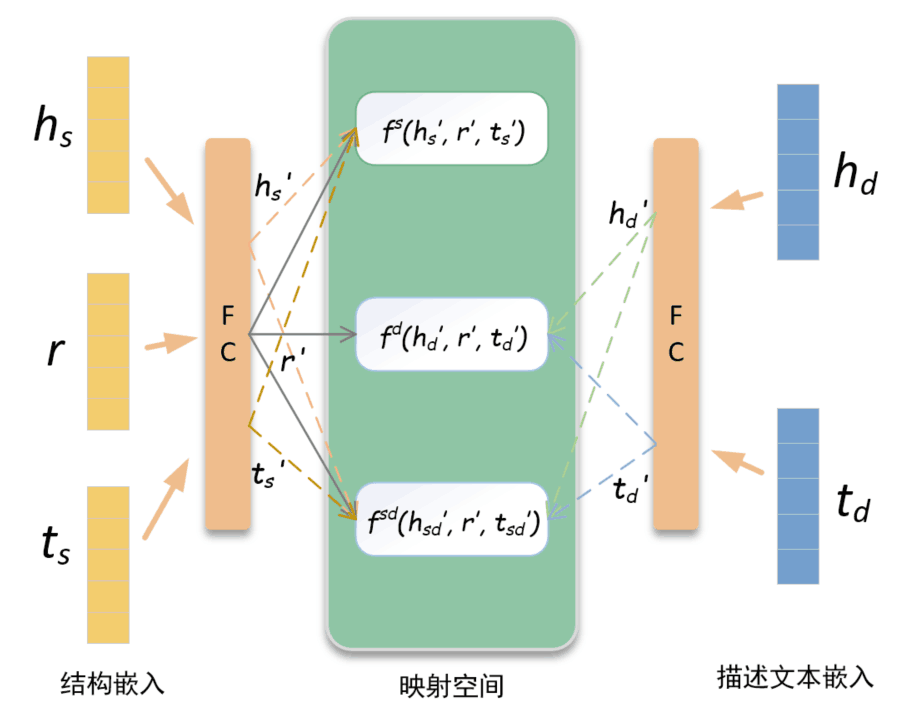
\includegraphics[width=0.9\textwidth]{3-2.png}
  \caption{本体嵌入架构}
  \label{fig:3-2}
\end{figure}

\section{关系嵌入模块}
\subsection{本体信息嵌入}
为了能从本体三元组的结构数据中捕捉到能够辅助实体三元组编码,特别是包含未见组件的本体概念信息,本文首先需要将本体三元组转换为响应的语义信息编码。与传统的知识图谱嵌入表示类似,对于一个本体三元组\((c_{i},p,c_{j})\),本体语义信息编码的目的就是设计出一个打分函数\(f(c_{i},p,c_{j})\)作为编码模型的激活函数,本文分别采用了传统的知识图谱嵌入方法如TransE对本体三元组进行编码,然后将编码后的本体信息用于辅助关系编码。例如按照TransE模型的设定,本体三元组的元关系属性是头尾两个实体节点的转移量,将打分函数设置为:
\begin{equation}
  f_{TransE}(c_{i},p,c_{j}) = - \| \textbf{c}_{i} + \textbf{p} + \textbf{c}_{j}\| \label{eq:3-1}
\end{equation}

其中\(\textbf{c}_{i}\),\(\textbf{p}\),\(\textbf{c}_{j}\),是一个本体三元组响应的概念编码和元关系编码。同时为了提高所有本体三元组的嵌入效果,本文采用自对抗负抽样损失函数来对计算损失更新模型:
\begin{equation}
  \mathcal{L}_{\mathcal{O}} = \frac{1}{\mid \mathcal{T}_{\mathcal{O}}\mid} \sum_{(c_{i},p,c_{j}) \in \mathcal{T}_{\mathcal{O}}} [\gamma _{o} + f(c'_{i},p,c'_{j}) + f(c_{i},p,c_{j})] \label{eq:3-2}
\end{equation}

公式中\(\gamma _{o}\)是控制正负样本得分的参数,同时\(c'_{i}\),\(c'_{j}\)是不存在与本体三元组中的负样本,为了生成这些负样本,本文在所有的本体概念中分别遮盖住已存在的本体三元组的头节点和尾结点,然后从所有本体节点中随机筛选出其他节点组成负样本。
本体信息除了结构化的本体三元组之外,还有许多对本体的详细描述文本,如本体节点“companyceo”的描述文本“specifies that a particular CEO is the CEO of a particular company”。这些描述文本可以在对本体信息提取的时候提供额外的语义信息,因此本文通过文本描述进一步加强了对本体三元组的语义嵌入。但是描述文本的建模和一般的三元组建模因为模型的差异一定无法直接进行融合,因此对于一个特定的本体三元组\((c_{i},p,c_{j})\),本文首先获得了三元组结构的嵌入\(h_{s}/r/t_{s} \in \mathbb{R}^{d_{1}}\)以及对每一个本体节点描述文本的向量表示\(h_{d}/t_{d} \in \mathbb{R}^{d_{2}}\)来指代文本描述信息,为了能够让这两个不同层面的嵌入进行融合,本文引入一个全连接层将两个不同的嵌入同时映射到同一个表示维度上,映射后的结构嵌入和文本嵌入分别表示为\(h_{s}^{'}\)和\(h_{d}^{'}\),在统一后的表示空间中使用TransE对三元组结构的嵌入进行打分:
\begin{equation}
  f^{s} = -  \parallel h'_{s} + r' - t'_{s}  \parallel \label{eq:3-3}
\end{equation}

对描述文本的嵌入进行打分:
\begin{equation}
  f^{d} = -  \parallel h'_{d} + r' - t'_{d}  \parallel \label{eq:3-4}
\end{equation}

同时为了为了使这两种类型的表示相互兼容和互补,本文遵循DKRL模型的设定来定义交叉和相加得分函数:
\begin{equation}
  f^{sd} = -  \parallel h'_{s} + r' - t'_{d}  \parallel -  \parallel h'_{d} + r' - t'_{s}  \parallel \label{eq:3-5}
\end{equation}

所有的四个得分函数综合可以保证两个层面的嵌入表示可以在相同空间里进行学习和更新,最后本体嵌入的得分函数表示为:
\begin{equation}
  f^{sd} = -  \parallel h'_{s} + r' - t'_{d}  \parallel -  \parallel h'_{d} + r' - t'_{s}  \parallel \label{eq:3-6}
\end{equation}

因此在本体嵌入的损失函数也响应的转化为:
\begin{equation}
  \mathcal{L}_{\mathcal{O}}^{ont} = \frac{1}{\mid \mathcal{T}_{\mathcal{O}}\mid} \sum_{(c_{i},p,c_{j}) \in \mathcal{T}_{\mathcal{O}}} [\gamma _{o} + f'(c'_{i},p,c'_{j}) + f'(c_{i},p,c_{j})] \label{eq:3-7}
\end{equation}

经过训练后每个本体节点都有两个层面的嵌入:三元组结构嵌入和描述文本嵌入,然后本文将这两种映射后的嵌入进行拼接作为本体节点的最终的向量表示。上述的描述文本的向量表示,本文采用了CNN网络进行生成。

\subsection{关系图构建}
对未见的关系,由于在训练集中没有相关的三元组可以提供特征学习的支持,所以必须要从除三元组以外的其他层面获取到可以对未见关系编码的特征表示。而关系作为构成知识图谱的一种结构信息,关系受相连节点的影响会与其他关系存在联系,这些联系可以作为关系的一种拓扑特征信息,类似的研究也有使用节点的度作为节点特征进行学习的尝试。这些结构性的信息会减少对训练集数据的依赖,在对关系特征进行学习的时候可以通过聚合相连其他关系的信息来对关系进行特征表示,能够较好作用在未见的关系上。

为了对关系的结构特征进行学习,本文继承了TACT模型对于关系的拓扑设定,将相邻的两个关系按照关系的方向抽取出四种元关系类型,并将关系视为节点,关系与关系之间由元关系进行连接。
\begin{figure}[h]
  \centering
  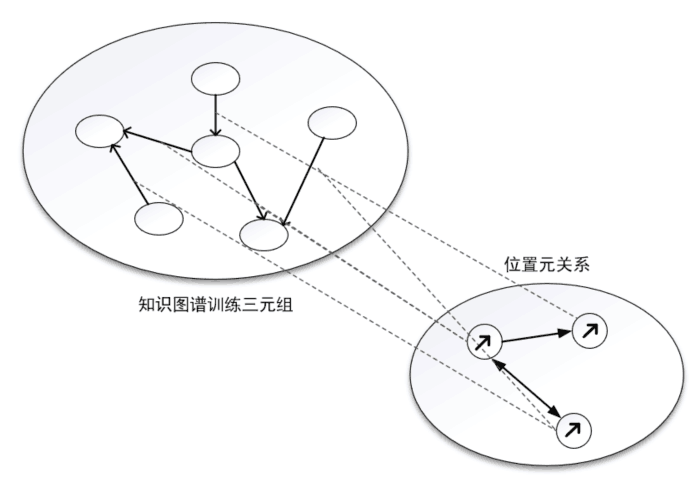
\includegraphics[width=0.5\textwidth]{3-3.png}
  \caption{从实体关系构建关系图}
  \label{fig:3-3}
\end{figure}

这些元关系根据关系的相对关系设置为四类,如图\ref{fig:3-4}所示,分别为tail-head、head-tail、tail-tail、head-head。元关系的head和tail都代表了两个相邻关系的指向,比如(relation1,tail-head,relation2)代表同一个实体连接的两个相邻关系1和关系2,且关系1指向该实体而关系2则从该实体指向其他实体。对于在训练三元组中的两个关系,如果它们符合其中一种的相对未见关系,则在关系位置图中创建一个关系结点,并通过与关系进行连接。
\begin{figure}[h]
  \centering
  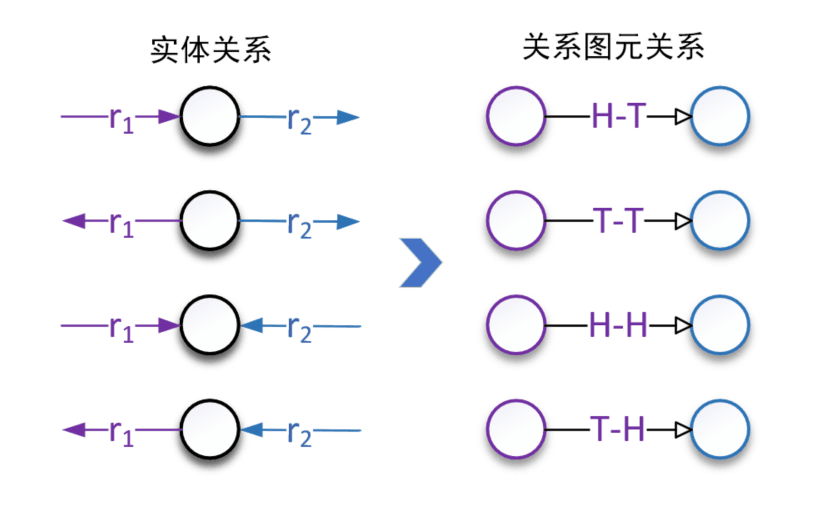
\includegraphics[width=0.5\textwidth]{3-4.png}
  \caption{实体关系与关系图元关系的映射}
  \label{fig:3-4}
\end{figure}

因此根据输入的实体三元组,可以将原始的图结构转变为关系相关图,同时在构建图的过程中没有使用到任何额外的实体属性或关系属性,可以作用到任何未见或已知的关系上。在关系相关图中的节点代表关系,边表示在原始三元组任意两个关系对应的元关系。

\subsection{关系相关性系数聚合编码}
在位置本体图中结点为原三元组中的关系,其位置结构部分的特征可以通过聚合关系结点的其他相邻关系结点的特征获取该关系的特征。为了能够将本体的嵌入作为对关系嵌入的语义补充,在构建好的关系位置图上本文通过对关系节点到本体概念的映射获取到各关系节点的初始化特征表示,然后通过多层GCN网络聚合邻接节点的特征来加强对关系节点的特征学习,对于节点的更新公式如下:
\begin{equation}
  h_{v} = f\left( \sum_{(u,r) \in \mathcal{N}(v)} W h_{u}\right) \label{eq:3-8}
\end{equation}

其中\(h_{u}\)是相邻关系节点的特征,每层GCN会有两步的操作,首先左乘归一化后的邻接矩阵对邻居节点的特征进行聚合,然后右乘一个可学习的线性转换矩阵\(W_{r}\)将输入的特征映射到目标特征空间中,最后使用一个非线性的激活函数来获取本层的特征输出。

为了区分在链接预测任务中不同元关系的的重要性,本文在对不同元关系连接的关系特征进行聚合时设置一个可学习的权重参数,根据任务的表现来学习不同元关系对应的重要程度,计算公式转化为:
\begin{equation}
  h_{v} = f\left( \sum_{(u,r) \in \mathcal{N}(v)} W_{ \lambda(r) } h_{u}\right) \label{eq:3-9}
\end{equation}

其中\(w_{r}\)是两个关系节点相连的元关系类型相对应的参数,根据本文设定的四种不同的元关系,该系数由四个不同的参数控制:
\begin{equation}
  W_{dir(r)} = \left\{ \begin{array}{rcl}
    &W_{t-h}  \mbox{,} &\quad r \in R_{tail-head} \\
    &W_{h-t}  \mbox{,} &\quad  r \in R_{head-tail} \\
    &W_{t-t}  \mbox{,} &\quad  r \in R_{tail-tail} \\
    &W_{h-h}  \mbox{,} &\quad  r \in R_{head-head} \\
    \end{array}\right\} \label{eq:3-10}
\end{equation}

\section{实体嵌入模块}
对于未见的实体特征提取,本文认为对一个未见的实体可通过它连接的关系来进行预测。如图\ref{fig:3-5}所示,右侧未见实体X的关系结构和Tom的关系相似,可以推断出3是一个类似Tom的一个学生节点,所以本文通过聚合实体所有关系来对实体进行表示。
\begin{figure}[h]
  \centering
  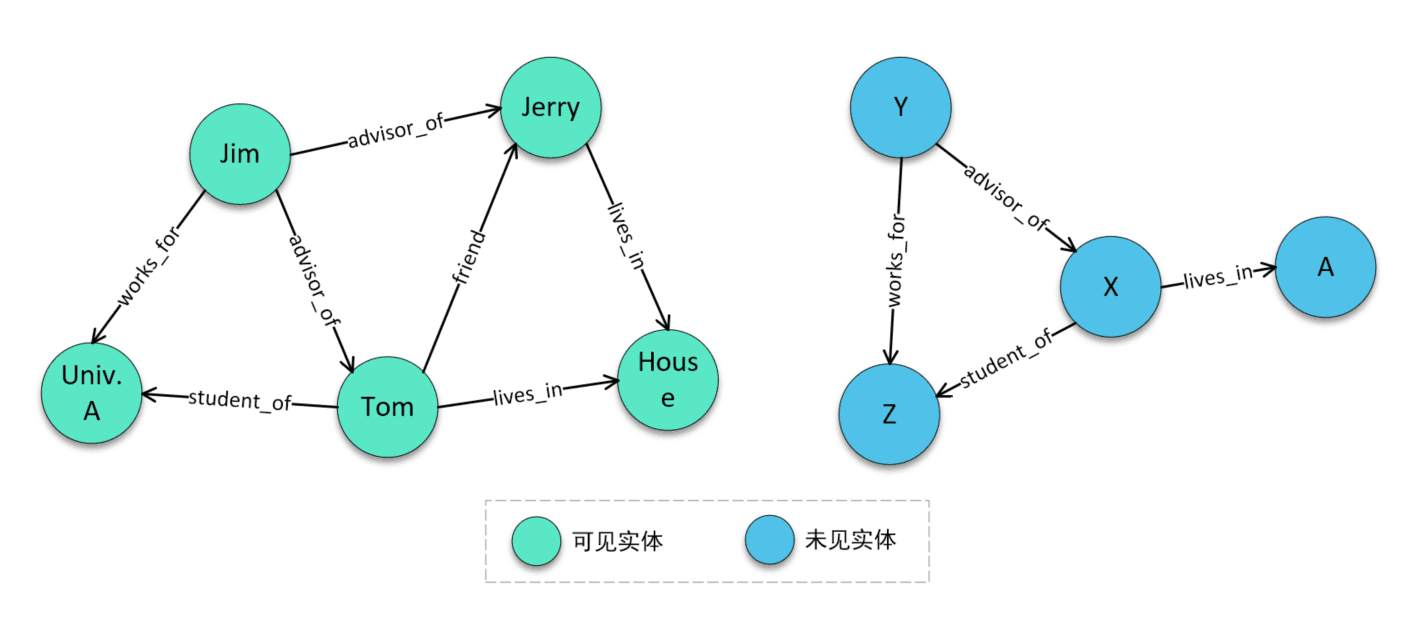
\includegraphics[width=0.8\textwidth]{3-5.png}
  \caption{未见实体的关系特征}
  \label{fig:3-5}
\end{figure}

同时考虑到实体关系的方向性,本文通过以下公式来进行实体特征的聚合:
\begin{equation}
  h_{e} = \frac{1}{ \mid \mathcal{N}(e) \mid} \sum_{r\in\mathcal{N}(e)} W^{ent}_{dir(r) }h_{r} \label{eq:3-11}
\end{equation}

\(\mathcal{N}(e)\)是实体e所有连接关系的集合;\(W^{ent}_{dir(r)}\)是用于将关系特征转化为实体特征且区分方向的一个转换参数,\(W^{ent}_{dir(r)}\)在关系r为指向实体e时表示为\(W^{ent}_{in}\),当关系r由实体e指向其他实体时记作\(W^{ent}_{out}\)。

\section{实体关系联合嵌入模块}
为了将关系特征聚合获得的实体特征进行抽取,本文在将输出的特征作为输入放到一个GNN网络中进行更新和编码得到学习后的嵌入,该GNN网络也以CompGCN模型为基础,但是将模型原有的实体关系聚合器修改为了一个线性转化层可以更好适应以多种传统KGE方法如RotatE来作为解码器进行下游任务,GNN层的实体嵌入更新如下:
\begin{equation}
  m _ { e } ^ { l + 1 } = \sum _ { ( r , t ) \in \mathcal{O} ( e ) } W _ { \text { out } } ^ { l } [ h _ { r } ^ { l } ; h _ { t } ^ { l } ] + \sum _ { ( r , h ) \in\mathcal{I} ( e ) } W _ { in } ^ { l } [ h _ { r } ^ { l } ; h _ { h } ^ { l } ]  \label{eq:3-12}
\end{equation}

\(\mathcal{O} ( e )\)是实体e的所有指向其他节点的关系和实体的集合,\(\mathcal{I} ( e )\)是所有指向其他节点e的关系和实体的集合,\( W _ { in } ^ { l }\)和\( W _ { out } ^ { l }\)分别是在GNN网络的第l层对实体的入关系和出关系的可学习的参数,\([;]\)而指代两个向量的连接操作。经由一层的GNN网络对特征的聚合后,实体的特征转换公式如下:
\begin{equation}
  h _ { e } ^ { l + 1 } = \sigma \left( \frac { m _ { e } ^ { l + 1 } } { | \mathcal{O} ( e ) | + | \mathcal{I} ( e ) | } + W _ { \text { self } } ^ { l } h _ { e } ^ { l } \right) \label{eq:3-13}
\end{equation}

\(W _ { \text { self } } ^ { l }\)是针对实体e本身特征自循环更新的模型学习参数,\(\sigma\)指代模型GNN模型的激活函数。同时,关系也在该层GCN中也进行了更新操作:
\begin{equation}
  h _ { r } ^ { l + 1 } = \sigma (W _ { \text { self } } ^ { l } h _ { r } ^ { l }) \label{eq:3-14}
\end{equation}

经过两层GCN对关系嵌入和实体嵌入的更新,该GNN模块即可输出该训练任务下所有可见组件以及未见组件的知识提取表示,用于本次任务的loss的计算及模型参数更新。

\section{元学习训练设定}
为了能够对知识图谱中的未见关系和未见实体进行表示学习,借鉴于元学习learning to learn的思想,本文从训练集中抽取了一系列包含未见实体和关系的训练任务来模拟测试环境,并且在该训练环境中对模型进行训练。

每个训练任务\(\mathcal{S}^{i} = (\mathcal{E}^{i}, \mathcal{R}^{i}, \mathcal{T}^{i}_{sup},\mathcal{T}^{i}_{que})\)包含训练实体集、关系集、support训练三元组集以及query测试三元组集。为了模拟未见的组件,将部分实体和关系标记为未见,每个训练任务被重新定义为如下:
\begin{equation}
  \mathcal{S}^{i} = (\mathcal{E}^{i} = (\hat{\mathcal{E}}^{i},\tilde{\mathcal{E}}^{i}), \mathcal{R}^{i} = (\hat{\mathcal{R}}^{i} ,\tilde{\mathcal{R}}^{i}   ), \mathcal{T}^{i}_{sup},\mathcal{T}^{i}_{que})  \label{eq:3-15}
\end{equation}

\(hat{\mathcal{E}}^{i} \in \mathcal{E}^{train}\)指代实体集中的可见实体而\(\tilde{\mathcal{E}}^{i} \notin \mathcal{E}^{train}\)指代未见的实体;\(\hat{\mathcal{R}}^{i} \in \mathcal{R}^{train}\)指代关系集中的可见关系\(\tilde{\mathcal{R}}^{i} \notin \mathcal{R}^{train}\)指代未见的关系。因此所有训练的总目标是基于每个任务的support集上进行对未见组件的训练使得在query集上的评估得分最高:
\begin{equation}
  \max\limits_{ \theta } \mathbb{E} _ { S ^ { i } \sim p ( S ) } \left[ \sum\limits_{ ( h , r , t ) \in \mathcal{T} _ { \text { que } } ^ { i } } \frac { 1 } { | \mathcal{T} _ { \text { que } } ^ { i } | } \mathcal{M} _ { \theta } ( h , r , t | \mathcal{T} _ { \text { sup } } ^ { i } ) \right] \label{eq:3-16}
\end{equation}

其中\(\mathcal{M}\)可以通过在support集上学习到响应的模型参数然后在query集上对三语组进行可行性打分,结合前几节模型中学习到的两个分散的embedding对三元组进行打分。本文采用自对抗负抽样损失函数来对计算损失更新模型:
\begin{equation}
\begin{aligned}
  \mathcal{L}(\mathcal{S}^{i}) = &\frac{1}{|\mathcal{T}^{i}_{que}|} \sum\limits_{(h,r,t)\in\mathcal{T}^{i}_{que}}-log\sigma(\gamma + s(h,r,t)) \\
  &-\sum\limits_{i=1}^{n}p(h'_{i},r,t'_{i})log\sigma(-\gamma - s(h,r,t)) \label{eq:3-17}
\end{aligned}
\end{equation}

n指代负采样的数量,\(p(h'_{i},r,t'_{i})\)指代负采样的权重系数,\(s(h,r,t)\)是用于计算embedding在query三元组上的得分函数。

\section{链接预测任务及训练流程}
链接预测任务主要是基于知识图谱已有事实来推断出知识图谱中当前不存在的事实三元组,根据待预测节点的不同可区分为头结点预测和尾结点预测,通过比较测试的事实三元组在模型预测的事实三元组排名中出现的概率来评估模型链接预测任务的好坏。本文在进行每次任务损失的过程中,通过正负样本的联合计算出损失,并以此进行梯度下降求解。负样本损失计算公式如下:
\begin{equation}
\mathcal{L}_{neg} = \sum_{i = 1}^{n} \left( softmax(W[s_{tail};s_{head}])log \sigma (- [s_{tail};s_{head}]) \right) \label{eq:3-18}
\end{equation}

其中\(s_{tail}\)和\(s_{head}\)是对一个测试三元组对应的尾结点负采样得分和头结点负采样得分,n代表负采样的数量,\([;]\)操作将正负样本的得分矩阵进行简单的连接操作,\(W\)是对得分进行微调的权重参数,本文默认设置为1。之后和正样本的得分求得算术平均即为该测试三元组的单个损失。

对于模型的训练流程,本文按照元学习单任务训练方法进行,每个任务的目标都是使该任务下的连接预测效果最优,具体流程如下:

\begin{enumerate}[label=\arabic*)]
  \item 初始化模型参数,主要包含了训练数据集中可见实体和关系的嵌入初始化、元关系的权重参数以及两个不同阶段的GCN层和CompGCN层的传递参数。
  \item 获得任务的支持集和查询集,主要从原训练集中抽取单个任务的子图,并划分为支持集和查询集,同时对关系和节点的标签进行设置以模拟出未见组件。
  \item 单次任务训练获得实体关系的嵌入,通过KGE模型计算查询集损失,通过损失函数进行梯度下降求解。
  \item 更新模型参数,重复下一个任务的训练直至效果不再更优。
  \item 对测试集进行模型测试,输出任务得分。
\end{enumerate}

\section{本章小结}
本章从本文模型的总体架构开始逐步详细介绍了模型的各个组成部分,包括主要的关系编码模块、实体编码模块以及元学习训练任务的定义和训练流程的说明。在关系编码模块说明了本文模型如何对关系的拓扑结构进行提取以及如何通过GCN层对关系的本体信息和拓扑信息进行融合学习,从而学习到未见关系的有效表示;在实体编码模块,通过未见实体的邻接关系的特征聚合进行表示,并且在实例知识图谱之上再次通过GNN来聚合其他关系和实体信息完成最后的特征表示。之后的章节中将对本文模型在测试数据集上进行充分的实验,检验本文模型的有效性。
\chapter{实验结果及分析}
在前文中,本文针对跨域知识图谱中存在未见实体和未见关系的问题,提出了一个基于本体信息和元学习的知识表示学习模型。同时针对跨域知识表示学习中知识图谱语义信息的不足,本文提出了一种基于关系拓扑结构和描述文本的本体嵌入框架,通过获取本体信息并与图结构信息联合学习,实现了对未见实体和未见关系的特征聚合。结合元学习和本体嵌入技术,能够有效地处理跨域知识图谱中新实体和新关系的表示。为了验证模型的有效性,本章主要验证和评估了本文模型(NAMER)的实验效果。实验主要面向跨域情景的测试数据集进行,与现有的处理类似问题的归纳知识图谱表示模型进行对比。结果表明,引入了多层次的特征信息后,本文模型在实验数据上明显优于其他现有模型。最后的多个消融实验也证明了模型各个组成部分的重要性。

\section{数据集}
由于传统的知识图谱数据集通常基于“closed-world”设定,测试三元组中的实体和关系在训练数据集中已知,不存在跨域场景中的未见实体和未见关系。因此,为测试模型在包含未知实体和关系的跨域场景下的有效性,本文通过抽取包含本体层次三元组的DBpedia和NELL-995知识图谱的子集构建了新的数据集DB\_Ext和NELL\_Ext。

\subsection{源数据集介绍}
DBpedia:DBpedia是一个基于维基百科的语义知识库。该数据集由开源社区维护并使用维基百科文章和其他在线网络资源进行扩展。DBpedia从Wikipedia中提取结构化的数据,转化为事实三元组进行存储,包括图像、标签、描述文本等结构化属性,最新的数据集快照含有8.5亿条事实三元组数据。此外,DBpedia注重本体论的构建,本体类型数共768个,主要包括人物、地点、工作、组织等概念。这些实体、属性和关系通常以RDF图的形式存储,标准查询语言为SPARQL。DBpedia开源社区提供网页公布数据集的最新版本和统计数据,同时支持各数据集版本的检索和下载,为研究者使用提供了便利。

NELL-995:NELL-995数据集是根据NELL知识库抽取用于知识图谱补全任务的基准数据集。NELL (Never Ending Language Learning)是由卡内基梅隆大学领导的自动化学习系统,旨在从互联网的非结构化文本中自动提取知识。基于NELL知识库,NELL-995数据集包含995个实体和129个关系,覆盖地理、医学、体育、音乐、文化等广泛领域。NELL-995数据集的实体和关系被细粒度分类,每个实体被分配到一组多层次的关系类型中。因此,NELL-995数据集是学习细粒度知识表示和关系推理模型的理想数据集。

\subsection{任务数据集构建}
为了抽取出包含未见实体和关系的数据子集,本文首先构建一个包含所有三元组的实例知识图谱,在其中随机选取100个根实体节点并将每个节点的10个相邻接点组成测试子图,将子图中1/10的实体和关系标记为测试集,并从训练集中剔除这些实体和关系相关的三元组作为测试三元组;最终每个数据集中都包含了两个基本的子知识图谱,训练知识图谱\(\mathcal{G}^{train}\)和测试图谱\(\mathcal{G}^{test}\),后者包含了训练图谱中不存在的实体和关系。此外,为了测试模型对未见关系及未见实体的单独学习性能,在测试集中的query集设置中,本文将测试三元组分为三类:1、所有测试三元组中只包含了未见的实体(unseen\_ent);2、所有测试三元组中只包含了未见的关系(unseen\_rel);3、所有测试三元组中同时包含了未见的实体和关系(unseen\_both)。两个数据集中的统计数据如表\ref{tab:4-1}所示。其中,DB\_Ext数据集包含243个仅含未见实体的测试三元组、10个仅含未见关系的三元组和243个同时包含两个未见组件的三元组;NELL\_Ext数据集包含565个仅含未见实体的测试三元组、12个仅含未见关系的三元组和115个同时包含两个未见组件的三元组。各数据集包含三元组的统计数量如表\ref{tab:4-1}所示。
\begin{table}[h]
  \caption{数据集统计数据(括号中为未见组件数量)}
  \label{tab:4-1}
  \resizebox{\textwidth}{!}{%
  \begin{tabular}{@{}cccccccc@{}}
  \toprule
  {\color[HTML]{333333} }         & \multicolumn{3}{c}{{\color[HTML]{333333} 训练图谱}}                                                             & \multicolumn{4}{c}{{\color[HTML]{333333} 测试图谱}}                                                                                                                                                                                \\ \cmidrule(l){2-8} 
  {\color[HTML]{333333} }         & {\color[HTML]{333333} 实体数}  & {\color[HTML]{333333} 关系数} & {\color[HTML]{333333} 三元组数}                      & {\color[HTML]{333333} 实体数}      & {\color[HTML]{333333} 关系数}     & {\color[HTML]{333333} \begin{tabular}[c]{@{}c@{}}support\\ 三元组数\end{tabular}} & {\color[HTML]{333333} \begin{tabular}[c]{@{}c@{}}query\\ 三元组数\end{tabular}} \\ \midrule
  {\color[HTML]{333333} NELL\_Ext} & {\color[HTML]{333333} 1583} & {\color[HTML]{333333} 153} & \multicolumn{1}{c|}{{\color[HTML]{333333} 5269}} & {\color[HTML]{333333} 851(753)} & {\color[HTML]{333333} 140(30)} & {\color[HTML]{333333} 2160}                                                   & {\color[HTML]{333333} 692}                                                  \\
  {\color[HTML]{333333} DB\_Ext}   & {\color[HTML]{333333} 795}  & {\color[HTML]{333333} 115} & \multicolumn{1}{c|}{{\color[HTML]{333333} 1508}} & {\color[HTML]{333333} 913(884)} & {\color[HTML]{333333} 128(46)} & {\color[HTML]{333333} 1930}                                                   & {\color[HTML]{333333} 496}                                                  \\ \bottomrule
  \end{tabular}%
  }
  \end{table}
% \begin{table}[h]
%   \caption{数据集统计数据(括号中为未见组件数量)}
%   \label{tab:4-1}
%   \resizebox{\textwidth}{!}{%
%   \begin{tabular}{cccccccc}
%   \hline
%                       & \multicolumn{3}{c}{训练图谱}                                                                                    & \multicolumn{4}{c}{测试图谱}                                                                                                                                                         \\ \cline{2-8} 
%   \multirow{-2}{*}{} & 实体数                         & 关系数                        & 三元组数                                             & 实体数                             & 关系数                            & \begin{tabular}[c]{@{}c@{}}support\\ 三元组数\end{tabular} & \begin{tabular}[c]{@{}c@{}}query\\ 三元组数\end{tabular} \\ \hline
%   NELL\_Ext          & {\color[HTML]{333333} 1583} & {\color[HTML]{333333} 153} & \multicolumn{1}{c|}{{\color[HTML]{333333} 5269}} & {\color[HTML]{333333} 851(753)} & {\color[HTML]{333333} 140(30)} & {\color[HTML]{333333} 2160}                            & {\color[HTML]{333333} 692}                           \\
%   DB\_Ext            & {\color[HTML]{333333} 795}  & {\color[HTML]{333333} 115} & \multicolumn{1}{c|}{{\color[HTML]{333333} 1508}} & {\color[HTML]{333333} 913(884)} & {\color[HTML]{333333} 128(46)} & {\color[HTML]{333333} 1930}                            & {\color[HTML]{333333} 496}                           \\ \hline
%   \end{tabular}%
%   }
%   \end{table}

\section{模型参数设置}
对于用于对比的基准模型,本文采用了相关论文给出的最优超参数设置,本文模型采用的相关参数设置如表\ref{tab:4-2}所示。
% \begin{table}[h]
%   \caption{模型超参数设置}
%   \label{tab:4-2}
%   \resizebox{\textwidth}{!}{%
%   \begin{tabular}{cc|cc|cc}
%   \hline
%   {\color[HTML]{333333} 本体嵌入参数}          & {\color[HTML]{333333} 设置值}     & {\color[HTML]{333333} 元学习训练参数}             & {\color[HTML]{333333} 设置值}    & {\color[HTML]{333333} 嵌入参数}       & {\color[HTML]{333333} 设置值} \\ \hline
%   {\color[HTML]{333333} lr}              & {\color[HTML]{333333} 0.00005} & {\color[HTML]{333333} lr}                  & {\color[HTML]{333333} 0.001}  & {\color[HTML]{333333} dim}        & {\color[HTML]{333333} 300} \\
%   {\color[HTML]{333333} ent\_str\_dim}     & {\color[HTML]{333333} 150}     & {\color[HTML]{333333} train\_bs}            & {\color[HTML]{333333} 64}     & {\color[HTML]{333333} num\_gcn}    & {\color[HTML]{333333} 2}   \\
%   {\color[HTML]{333333} ent\_text\_dim}    & {\color[HTML]{333333} 300}     & {\color[HTML]{333333} eval\_bs}             & {\color[HTML]{333333} 16}     & {\color[HTML]{333333} num\_comgcn} & {\color[HTML]{333333} 2}   \\
%   {\color[HTML]{333333} mapping\_size}    & {\color[HTML]{333333} 300}     & {\color[HTML]{333333} num\_step}            & {\color[HTML]{333333} 100000} & {\color[HTML]{333333} gcn\_dim}    & {\color[HTML]{333333} 300} \\
%   {\color[HTML]{333333} training\_epochs} & {\color[HTML]{333333} 1000}    & {\color[HTML]{333333} early\_stop\_patience} & {\color[HTML]{333333} 20}     & {\color[HTML]{333333} hid\_drop}   & {\color[HTML]{333333} 0.3} \\
%   {\color[HTML]{333333} batch\_size}      & {\color[HTML]{333333} 100}     & {\color[HTML]{333333} num\_sample\_size}     & {\color[HTML]{333333} 10}     & {\color[HTML]{333333} -}          & {\color[HTML]{333333} -}   \\ \hline
%   \end{tabular}%
%   }
%   \end{table}
% \begin{table}[h]
%   \caption{模型超参数设置}
%   \label{tab:4-2}
%   \resizebox{\textwidth}{!}{%
%   \begin{tabular}{|c|c|c|c|c|c|}
%   \hline
%   {\color[HTML]{333333} 本体嵌入参数}           & {\color[HTML]{333333} 设置值}     & {\color[HTML]{333333} 元学习训练参数}                          & {\color[HTML]{333333} 设置值}    & {\color[HTML]{333333} 嵌入参数}        & {\color[HTML]{333333} 元学习训练参数} \\ \hline
%   {\color[HTML]{333333} lr}               & {\color[HTML]{333333} 0.00005} & {\color[HTML]{333333} lr}                               & {\color[HTML]{333333} 0.001}  & {\color[HTML]{333333} dim}         & {\color[HTML]{333333} 300}     \\ \hline
%   {\color[HTML]{333333} ent\_str\_dim}    & {\color[HTML]{333333} 150}     & {\color[HTML]{333333} train\_bs}                        & {\color[HTML]{333333} 64}     & {\color[HTML]{333333} num\_gcn}    & {\color[HTML]{333333} 2}       \\ \hline
%   {\color[HTML]{333333} ent\_text\_dim}   & {\color[HTML]{333333} 300}     & {\color[HTML]{333333} eval\_bs}                         & {\color[HTML]{333333} 16}     & {\color[HTML]{333333} num\_comgcn} & {\color[HTML]{333333} 2}       \\ \hline
%   {\color[HTML]{333333} mapping\_size}    & {\color[HTML]{333333} 300}     & {\color[HTML]{333333} num\_step}                        & {\color[HTML]{333333} 100000} & {\color[HTML]{333333} gcn\_dim}    & {\color[HTML]{333333} 300}     \\ \hline
%   {\color[HTML]{333333} training\_epochs} & {\color[HTML]{333333} 1000}    & {\color[HTML]{333333} early\_stop\_patience}            & {\color[HTML]{333333} 20}     & {\color[HTML]{333333} hid\_drop}   & {\color[HTML]{333333} 0.3}     \\ \hline
%   {\color[HTML]{333333} batch\_size}      & {\color[HTML]{333333} 100}     & {\color[HTML]{333333} num\_sample\_for\_estimate\_size} & {\color[HTML]{333333} 10}     & {\color[HTML]{333333} -}           & {\color[HTML]{333333} -}       \\ \hline
%   \end{tabular}%
%   }
% \end{table}

其中主要包含以下三个方面的参数设置:
\begin{enumerate}[label=\arabic*)]
\item 本体嵌入相关参数:模型学习率lr、本体三元组概念节点结构嵌入维度ent\_str\_dim、本体概念节点文本嵌入维度ent\_text\_dim、线性隐藏层维度mapping\_size以及训练的epoch数量和batch的大小。
\item 元学习相关参数:任务学习率lr、单任务支持集的batch数量train\_bs、单任务查询集的batch数量eval\_bs、元训练总任务数num\_step、元训练提前结束无效训练任务计数early\_stop\_patience以及单个batch采样的根节点数。
\item 图谱嵌入相关参数:基本维度的设置dim、关系位置图对关系进行GCN的层数num\_gcn、GCN中间传递维度gcn\_dim以及GCN层的丢弃率hid\_drop、对关系和实体进行联合学习的CompGCN的层数num\_compgcn。
\end{enumerate}
\begin{table}[h]
  \caption{模型超参数设置}
  \label{tab:4-2}
  \resizebox{\textwidth}{!}{%
  \begin{tabular}{@{}cccccc@{}}
  \toprule
  {\color[HTML]{333333} \textbf{本体嵌入参数}} & {\color[HTML]{333333} \textbf{设置值}}                 & {\color[HTML]{333333} \textbf{元学习训练参数}}    & {\color[HTML]{333333} \textbf{设置值}}                & {\color[HTML]{333333} \textbf{嵌入参数}} & {\color[HTML]{333333} \textbf{设置值}} \\ \midrule
  {\color[HTML]{333333} lr}              & \multicolumn{1}{c|}{{\color[HTML]{333333} 0.00005}} & {\color[HTML]{333333} lr}                  & \multicolumn{1}{c|}{{\color[HTML]{333333} 0.001}}  & {\color[HTML]{333333} dim}           & {\color[HTML]{333333} 300}          \\
  {\color[HTML]{333333} ent\_str\_dim}     & \multicolumn{1}{c|}{{\color[HTML]{333333} 150}}     & {\color[HTML]{333333} train\_bs}            & \multicolumn{1}{c|}{{\color[HTML]{333333} 64}}     & {\color[HTML]{333333} num\_gcn}       & {\color[HTML]{333333} 2}            \\
  {\color[HTML]{333333} ent\_text\_dim}    & \multicolumn{1}{c|}{{\color[HTML]{333333} 300}}     & {\color[HTML]{333333} eval\_bs}             & \multicolumn{1}{c|}{{\color[HTML]{333333} 16}}     & {\color[HTML]{333333} num\_compgcn}    & {\color[HTML]{333333} 2}            \\
  {\color[HTML]{333333} mapping\_size}    & \multicolumn{1}{c|}{{\color[HTML]{333333} 300}}     & {\color[HTML]{333333} num\_step}            & \multicolumn{1}{c|}{{\color[HTML]{333333} 100000}} & {\color[HTML]{333333} gcn\_dim}       & {\color[HTML]{333333} 300}          \\
  {\color[HTML]{333333} training\_epochs} & \multicolumn{1}{c|}{{\color[HTML]{333333} 1000}}    & {\color[HTML]{333333} early\_stop\_patience} & \multicolumn{1}{c|}{{\color[HTML]{333333} 20}}     & {\color[HTML]{333333} hid\_drop}      & {\color[HTML]{333333} 0.3}          \\
  {\color[HTML]{333333} batch\_size}      & \multicolumn{1}{c|}{{\color[HTML]{333333} 100}}     & {\color[HTML]{333333} num\_sample\_size}     & \multicolumn{1}{c|}{{\color[HTML]{333333} 10}}     & {\color[HTML]{333333} -}             & {\color[HTML]{333333} -}            \\ \bottomrule
  \end{tabular}%
  }
  \end{table}

在对三元组进行打分评估时,本文通过对CompGCN第二层输出的改进,可支持多种KGE模型作为评分函数。实际采用的KGE模型包含TransE、DistMult、ComplEx及RotatE。实体和关系的维度根据采用的KGE模型在基础嵌入维度上进行调整,具体如下表\ref{tab:4-3}所示:
\begin{table}[h]
  \caption{评分函数}
  \label{tab:4-3}
  \centering
  \resizebox{0.6\textwidth}{!}{%
  \begin{tabular}{@{}cccc@{}}
  \toprule
  {\color[HTML]{333333} \textbf{模型名}} & {\color[HTML]{333333} \textbf{实体维度}} & {\color[HTML]{333333} \textbf{关系维度}} & {\color[HTML]{333333} \textbf{评分函数}}        \\ \midrule
  {\color[HTML]{333333} TranE}        & {\color[HTML]{333333} dim}           & {\color[HTML]{333333} dim}           & {\color[HTML]{333333} F = -|| h + r - t ||} \\
  {\color[HTML]{333333} DistMult}     & {\color[HTML]{333333} dim}           & {\color[HTML]{333333} dim}           & {\color[HTML]{333333} F = \(\rm h^{T}\) diag(r) t}     \\
  {\color[HTML]{333333} ComplEx}      & {\color[HTML]{333333} 2 * dim}       & {\color[HTML]{333333} 2 * dim}       & {\color[HTML]{333333} F = Re(\(\rm h^{T}\) diag(r) t)} \\
  {\color[HTML]{333333} RotatE}       & {\color[HTML]{333333} 2 * dim}       & {\color[HTML]{333333} dim}           & {\color[HTML]{333333} F = -|| h ○ r - t ||} \\ \bottomrule
  \end{tabular}%
  }
  \end{table}
% \begin{table}[h]
%   \caption{评分函数}
%   \label{tab:4-3}
%   \centering
%   \resizebox{0.7\textwidth}{!}{%
%   \begin{tabular}{cccc}
%   \hline
%   {\color[HTML]{333333} 模型名}      & {\color[HTML]{333333} 实体维度}    & {\color[HTML]{333333} 关系维度}    & {\color[HTML]{333333} 评分函数}                 \\ \hline
%   {\color[HTML]{333333} TranE}    & {\color[HTML]{333333} dim}     & {\color[HTML]{333333} dim}     & {\color[HTML]{333333} F = -|| h + r - t ||} \\
%   {\color[HTML]{333333} DistMult} & {\color[HTML]{333333} dim}     & {\color[HTML]{333333} dim}     & {\color[HTML]{333333} F = \(\rm h^{T}\) diag(r) t}     \\
%   {\color[HTML]{333333} ComplEx}  & {\color[HTML]{333333} 2 * dim} & {\color[HTML]{333333} 2 * dim} & {\color[HTML]{333333} F = Re(\(\rm h^{T}\) diag(r) t)} \\
%   {\color[HTML]{333333} RotatE}   & {\color[HTML]{333333} 2 * dim} & {\color[HTML]{333333} dim}     & {\color[HTML]{333333} F = -|| h ○ r - t ||} \\ \hline
%   \end{tabular}%
%   }
%   \end{table}
% \begin{table}[h]
%   \caption{评分函数}
%   \label{tab:4-3}
%   \centering
%   \resizebox{0.8\textwidth}{!}{%
%   \begin{tabular}{|l|l|l|l|}
%   \hline
%   {\color[HTML]{333333} 模型名}      & {\color[HTML]{333333} 实体维度}    & {\color[HTML]{333333} 关系维度}    & {\color[HTML]{333333} 评分函数}                 \\ \hline
%   {\color[HTML]{333333} TranE}    & {\color[HTML]{333333} dim}     & {\color[HTML]{333333} dim}     & {\color[HTML]{333333} F = -|| h + r - t ||} \\ \hline
%   {\color[HTML]{333333} DistMult} & {\color[HTML]{333333} dim}     & {\color[HTML]{333333} dim}     & {\color[HTML]{333333} F = \(\rm h^{T}\) diag(r) t}     \\ \hline
%   {\color[HTML]{333333} ComplEx}  & {\color[HTML]{333333} 2 * dim} & {\color[HTML]{333333} 2 * dim} & {\color[HTML]{333333} F = Re(\(\rm h^{T}\) diag(r) t)} \\ \hline
%   {\color[HTML]{333333} RotatE}   & {\color[HTML]{333333} 2 * dim} & {\color[HTML]{333333} dim}     & {\color[HTML]{333333} F = -|| h ○ r - t ||} \\ \hline
%   \end{tabular}%
%   }
% \end{table}

其中评分函数中的h、r、t分别指代头实体、关系和尾实体的嵌入表示,Re表示复向量的实部分量,○操作表示旋转操作。

\section{实验设计及评价指标}
本实验包含本体嵌入表示学习和图谱表示学习两个阶段,第一个阶段主要学习到融合描述文本信息的本体嵌入表示,第二阶段使用本体信息进行跨域知识图谱的表示学习。

第一阶段首先采用传统的表示学习方法对本体三元组数据进行初步嵌入表示。其次,从预训练词嵌入glove中获取本体描述信息中各描述单词的初始化词向量。使用TF-IDF统计方法识别单词的重要程度,并对单词的词向量进行加权聚合计算,以获得本体节点描述文本的初始化向量嵌入。最后,将本体三元组的结构化表示嵌入和本体描述文本的表示嵌入映射到同一个空间,以进行评分和更新,从而获得拼接后的最终本体嵌入。

第二阶段对跨域知识图谱进行表示学习,为了在元学习中模拟出跨域场景,在每个元学习任务的设置中都人为抹除了一些实体和关系的标签,使得这些实体和关系必须通过本文模型的未见关系和未见实体嵌入模块学习得到向量表示,而不是从传统嵌入方法的嵌入矩阵中取得。

对于模型在链接预测任务上的评价指标,本文选取了MRR和Hit@10作为评判的标准。其中MRR通过预测三元组排名的倒数来进行计算,即对测试三元组中的所有事实三元组,如果该三元组在预测排名靠前,对应的倒数也会比较大,因此链接预测性能与MRR评价指标的数值大小成正相关。而Hits@n描述的是在所有预测三元组排名中前n的三元组所占的平均比例,其计算公式如公式\ref{eq:5-1}所示:
\begin{equation}
  HITS@n = \frac{1}{|S|} \sum_{i=1}^{|S|}||(rank_{i} \leqslant n) \label{eq:5-1}
\end{equation}

假设n设置为10,那么统计事实三元组在预测三元组中前n名的个数,最后再除以总个数就得到了Hits@10的结果,其中\(||(·)\)为indicator函数(若条件真则函数值为1,否则为0)。

参与比较的模型如下:

Neural-LP\cite{yang2017differentiable}(2017):该模型基于知识库构建了一个可学习逻辑规则的可微模型。逻辑规则是独立于实体和关系的,因此理论上该模型可在任何未见的实体上应用,并在归纳图谱补全任务中相比传统方法(即对实体进行结构信息表示学习)有明显提升。

DURM\cite{sadeghian2019drum}(2019):提出了一种可微的、可同时学习规则逻辑及其置信度得分的方法。该方法可以使用梯度优化来处理归纳逻辑编程任务,并可用于处理含有未知实体的链接预测任务。

GraIL\cite{teru2020inductive}(2020):该模型不直接学习实体节点嵌入,也没有使用任何节点的属性。相反,它在测试三元组候选关系的周围构建子图,并利用子图的结构和结构化的节点特征来预测三元组。这使得该模型能够很好地应用于未知的实体三元组预测任务。

CoMPILE\cite{mai2021communicative}(2021):该模型对GraIL模型子图归纳模型进行了改进,包括加强对子图关系方向性的限制,并在未知节点特征聚合的信息传递过程中增加了先前模型中忽略的关系特征。

MaKEr\cite{chen2019meta}(2022):该模型通过学习关系结构的特征来聚合邻接关系的特征,进而对关系进行表示,并聚合关系特征对实体进行编码。模型利用拓扑结构的信息,在一定程度上实现对未见实体和未见关系的表示。

\section{实验结果及分析}
各模型在NELL\_Ext上的链接预测任务实验结果如下表\ref{tab:4-4}所示,各模型在DB\_Ext上的链接预测任务实验结果如表\ref{tab:4-5}所示。根据测试数据集的三元组对未知实体和关系的包含情况,将结果分为了只包含未见实体的结果(u\_ent)、只包含未见关系的结果(u\_rel)以及同时包含未见实体和未见关系的结果(u\_both)。表格中加粗部分为最优的实验效果,带有下划线的则是该类基准模型中表现最优的得分,模型括号中指代的是在评分阶段采用的KGE评分函数。
\begin{table}[h]
  \caption{NELL\_Ext数据集结果}
  \label{tab:4-4}
  \resizebox{\textwidth}{!}{%
  \begin{tabular}{ccccccc}
  \hline
  \multicolumn{7}{c}{NELL\_Ext}                                                                                                                 \\ \hline
 {\multirow{2}{*}{}} & \multicolumn{2}{c}{u\_ent}       & \multicolumn{2}{c}{u\_rel}       & \multicolumn{2}{c}{u\_both}      \\ \cline{2-7} 
               & MRR            & Hits@10        & MRR            & Hits@10        & MRR            & Hits@10        \\ \hline
  \multicolumn{1}{c|}{Neural-LP}         & 30.48          & 47.96          & -              & -              & -              & -              \\
  \multicolumn{1}{c|}{DRUM}              & 31.82          & 48.32          & -              & -              & -              & -              \\
  \multicolumn{1}{c|}{GraIL}             & 71.62          & 92.92          & -              & -              & -              & -              \\
  \multicolumn{1}{c|}{CoMPILE}           & {\ul 75.94}    & {\ul 93.62}    & -              & -              & -              & -              \\ \hline
  \multicolumn{1}{c|}{MaKEr(TransE)}     & 70.82          & 92.00          & 24.56          & 54.17          & 21.53          & 51.74          \\
  \multicolumn{1}{c|}{MaKEr(DistMult)}   & 70.63          & 91.33          & 27.02          & 60.00          & \textbf{41.39} & 57.65          \\
  \multicolumn{1}{c|}{MaKEr(ComplEx)}    & 72.24          & 91.91          & 18.27          & 34.17          & 29.39          & 59.65          \\
  \multicolumn{1}{c|}{MaKEr(RotatE)}     & {\ul 77.09}    & {\ul 94.64}    & {\ul 31.53}    & {\ul 55.00}    & 31.45          & {\ul 62.35}    \\ \hline
  \multicolumn{1}{c|}{NAMER(TransE)}     & 78.28          & 94.69          & 20.72          & 53.34          & 27.11          & 55.85          \\
  \multicolumn{1}{c|}{NAMER(DistMult)}   & 75.98          & 92.46          & 19.30          & 22.50          & 31.37          & 55.65          \\
  \multicolumn{1}{c|}{NAMER(ComplEx)}    & 73.61          & 90.60          & 14.44          & 38.33          & 29.70          & 54.96          \\
  \multicolumn{1}{c|}{NAMER(RotatE)}     & \textbf{79.92} & \textbf{94.73} & \textbf{45.07} & \textbf{75.63} & {\ul 40.33}    & \textbf{67.06} \\ \hline
  \end{tabular}%
  }
  \end{table}
\begin{table}[h]
  \caption{DB\_Ext数据集结果}
  \label{tab:4-5}
  \resizebox{\textwidth}{!}{%
  \begin{tabular}{ccccccc}
  \hline
  \multicolumn{7}{c}{DB\_Ext}                                                                                                                 \\ \hline
                 & \multicolumn{2}{c}{u\_ent}       & \multicolumn{2}{c}{u\_rel}       & \multicolumn{2}{c}{u\_both}      \\ \cline{2-7} 
               & MRR            & Hits@10        & MRR            & Hits@10        & MRR            & Hits@10        \\ \hline
  \multicolumn{1}{c|}{Neural-LP}       & 57.15          & 73.46          & -              & -              & -              & -              \\
  \multicolumn{1}{c|}{DRUM}            & 59.88          & 73.25          & -              & -              & -              & -              \\
  \multicolumn{1}{c|}{GraIL}           & 59.44          & {\ul 80.86}    & -              & -              & -              & -              \\
  \multicolumn{1}{c|}{CoMPILE}         & {\ul 60.66}    & 79.93          & -              & -              & -              & -              \\ \hline
  \multicolumn{1}{c|}{MaKEr(TransE)}   & 54.4           & 83.7           & 31.13          & 54.00          & 38.66          & 66.50           \\
  \multicolumn{1}{c|}{MaKEr(DistMult)} & 46.24          & 81.07          & 16.43          & 11.00          & 32.16          & 56.71          \\
  \multicolumn{1}{c|}{MaKEr(ComplEx)}  & 53.79          & 82.47          & 19.95          & 29.00          & 36.88          & 59.26          \\
  \multicolumn{1}{c|}{MaKEr(RotatE)}   & {\ul 59.55}    & {\ul 86.09}    & {\ul 32.93}    & {\ul 55.00}    & \textbf{41.27} & {\ul 66.54}    \\ \hline
  \multicolumn{1}{c|}{NAMER(TransE)}   & 64.63          & 89.60          & \textbf{44.77} & 70.25          & 34.92          & \textbf{69.42} \\
  \multicolumn{1}{c|}{NAMER(DistMult)} & 56.73          & 80.25          & 13.68          & 11.00          & 33.94          & 61.74          \\
  \multicolumn{1}{c|}{NAMER(ComplEx)}  & 52.22          & 77.34          & 14.40          & 15.00          & 31.72          & 59.49          \\
  \multicolumn{1}{c|}{NAMER(RotatE)}   & \textbf{66.43} & \textbf{89.67} & 41.80          & \textbf{74.00} & {\ul 35.11}    & 63.81          \\ \hline
  \end{tabular}%
  }
\end{table}

表\ref{tab:4-4}和表\ref{tab:4-5}展示了各模型在NELL\_Ext和DB\_Ext上的链接预测结果。计算Hit@10分数时,本文选取了50个候选进行评估,并对于不同的补全任务(u\_ent、u\_rel和u\_both)显示了不同模型的得分。GraIL、Neural-LP、DRUM和CoMPILE仅针对未见实体补全任务设计了实验,因此未列出其在未见关系上的实验结果。上述数据均为模型运行4次后取平均值的结果。

结果表明,本文提出的NAMER模型相比其他基准模型有所改进,并在不同的KGE评分模型上有不同程度的提升。此外,基于RotatE的NAMER模型总体取得了最好的成绩。我们认为RotatE模型采用了更加复杂的关系和实体的映射关系,因此能表现更多没有重叠的特征信息。这也证明了本文模型的有效性。

本文在处理未见实体的测试集上,首先比较了依据规则学习来处理未见实体的Neural-LP模型和DRUM模型以及基于子图推理的GraIL模型和CoMPILE模型。结果表明,基于规则的模型的效果不如基于子图的模型,在 NELL\_Ext 数据集上,Neural-LP和DRUM的实验得分远低于GraIL和CoMPILE模型。这是由于基于规则的模型依赖于针对数据集学习出的规则,需要大量的数据集或对样本均衡性有严格的要求,因此模型效果受数据集影响较大。CoMPILE模型在GraIL模型的基础上强调了关系的重要性,总体效果要比GraIL表现更好。然而,上述四个模型都无法处理未见关系,而基于子图归纳推理的模型强调测试三元组中头尾实体间的局部子图信息,没有完全利用到实体周围的结构特征信息以及关系信息,整体效果都比本文的模型差。比较本文的模型与MaKEr模型,MaKEr模型在MRR的评价指标上平均低了4.42\%,而在对应RotatE评分函数下的Hits@10评价指标上,本文模型表现领先了1.85\%。尽管MaKEr模型考虑到了关系对实体的重要性,但在关系表示的特征学习方面,没有充分利用图谱的语义知识,所以效果比本文模型差。这进一步说明了本文模型在未见实体表示方面的有效性。

本文在仅包含未见关系和同时包含未见实体和关系的测试集上,与通过结构信息对关系和实体进行编码的MaKEr模型进行了比较。针对未知关系,本文引入了额外的本体知识作为关系语义信息的补充,并利用关系图卷积对关系的表示进行了更新,以学习未见关系周围的结构拓扑信息。两个测试集上的实验结果表明,相比于仅使用结构信息编码关系的MaKEr模型,本文引入本体信息能够有效补充关系表示的语义信息。在处理未知关系时,本文采用RotatE作为评分函数的模型表现出明显的优势,在NELL\_Ext数据集上的MRR得分比MaKEr高出14.54\%,而在Hits@10的得分方面,70.63的得分比MaKEr的得分高出约20\%。这表明本文模型在捕捉关系语义和结构信息方面具有更好的性能,在考虑局部关系和全局关系时都表现良好。在同时包含两种未知组件的测试集上,本文模型相比MaKEr模型在NELL\_Ext数据集的Hits@10评分上平均提升了1.82\%,在DB\_Ext数据集的MRR和Hits@10分别平均提升了1.18\%和0.53\%。

此外,本文实验发现,相比于DistMult和ComplEx模型,将TransE和RotatE用作解码器时模型效果更好,尤其在处理关系方面。在本体嵌入实验中,本文采用RotatE作为评分函数来对本体信息进行表示学习。DistMult和ComplEx模型因其复杂性与RotatE的本体嵌入方法不兼容而效果下降。相比之下,TransE模型简单易操作,在进行特征提取时更为适合。与本文模型搭配整体表现最好的RotatE模型不仅与本体嵌入方法相匹配,还能够提供更全面的对实体和关系低维度嵌入表示,因此在本文中表现为最优的模型之一。

\section{模型消融实验}
本节将介绍模型中几个重要模块的多项消融实验,以展示本文模型各部分的重要性,主要设置了5项不同的消融设置实验:(1)去除元学习的设置;(2)去除本体的设置;(3)去除实体聚合表示的设置;(4)去除关系GCN聚合的设置;(5)同时去除本体和元学习的设置。获得的实验结果如表\ref{tab:4-6}所示:
\begin{table}[h]
  \caption{在NELL\_Ext上的消融实验结果}
  \resizebox{\textwidth}{!}{%
  \label{tab:4-6}
  \begin{tabular}{ccccccc}
  \hline
  \multicolumn{7}{c}{NELL\_Ext}                                                                                                                  \\ \hline
                    & \multicolumn{2}{c}{u\_ent}       & \multicolumn{2}{c}{u\_rel}       & \multicolumn{2}{c}{u\_both}      \\ \cline{2-7} 
                 & MRR            & Hits@10        & MRR            & Hits@10        & MRR            & Hits@10        \\ \hline
  \multicolumn{1}{c|}{NAMER(TransE)}      & \textbf{78.28} & \textbf{94.86} & 20.72          & 53.34          & \textbf{27.11} & \textbf{55.85} \\ \hline
  \multicolumn{1}{c|}{no\_meta\_TransE}     & 29.31          & 43.82          & 12.65          & 30.83          & 10.18          & 22.26          \\
  \multicolumn{1}{c|}{no\_ont\_TransE}      & 76.89          & 94.07          & 14.96          & 27.50          & 14.06          & 28.78          \\
  \multicolumn{1}{c|}{no\_ent\_TransE}      & 76.85          & 94.07          & 18.00          & 55.83          & 19.43          & 50.7           \\
  \multicolumn{1}{c|}{no\_gcn\_TransE}      & 74.68          & 92.27          & \textbf{23.88} & \textbf{61.67} & 19.85          & 46.26          \\
  \multicolumn{1}{c|}{no\_meta\_ont\_TransE} & 26.57          & 38.69          & 11.15          & 25.00          & 12.62          & 27.74          \\ \hline
  \end{tabular}%
  }
  \end{table}

其中每个消融实验的具体设置如下:
\begin{enumerate}[label=\arabic*)]
  \item 去除元学习的设置:在模型训练阶段,本文引入了元学习,在训练集上提取任务子图并通过随机标签来模拟出未见的组件从而训练出模型处理未见组件的能力。在该消融实验下,取消掉了对子图标签的模拟效果即按照传统KGE模型的训练方法,在训练集上对所有三元组进行嵌入和损失计算。
  \item 去除本体的设置:本文模型的一个创新点即在对关系嵌入表示的时候通过关系位置图加入本体信息进行学习,在该消融实验设置下,将本体信息替换为随机表示对未见关系进行特征学习。
  \item 去除实体聚合表示的设置:本文模型在处理未见实体时,采用该实体周围的关系信息聚合表示,在该消融实验设置下对未见实体进行随机化嵌入设置,考察未见实体的表示模块。
  \item 去除关系GCN聚合的设置:在构建完关系的位置图并引入本体嵌入后,本文模型通过GCN来加强关系对邻接结构的特征学习,该消融实验下去除两层GCN层,直接使用本体信息。
  \item 同时去除本体和元学习设置:同时结合消融实验(1)和(2)的设置。
\end{enumerate}

将消融实验结果与NAMER(TransE)模型在NELL\_Ext上的实验结果进行比较,可以看出,基本所有的消融设置都会导致性能下降,表明上述各模块的重要性。但是在去除关系GCN聚合的设置上,在仅含有未见关系的测试集上效果反而提升,分析可知该层GCN的作用是在关系本体嵌入的基础上学习关系邻接关系的结构信息。这些结构信息的引入一定程度上会影响仅对关系的表示效果,导致在仅包含未见关系的测试集上的效果下降。但是这些结构信息的引入在未见实体的表示中,因为实体需要聚合邻接关系进行表示,因此引入的结构信息会对实体的表示效果进行提升,可以发现去掉GCN在包含未见实体和同时包含未见实体和未见关系的测试集上效果都有明显的下降,因此也侧面证明了GCN模型对实验效果提升的必要性。此外,本文观察到元学习设置对模型性能至关重要,表明在推广到测试知识图谱的任务上对模型进行元训练的有效性。

\section{未见实体案例分析}
\begin{figure}[h]
  \centering
  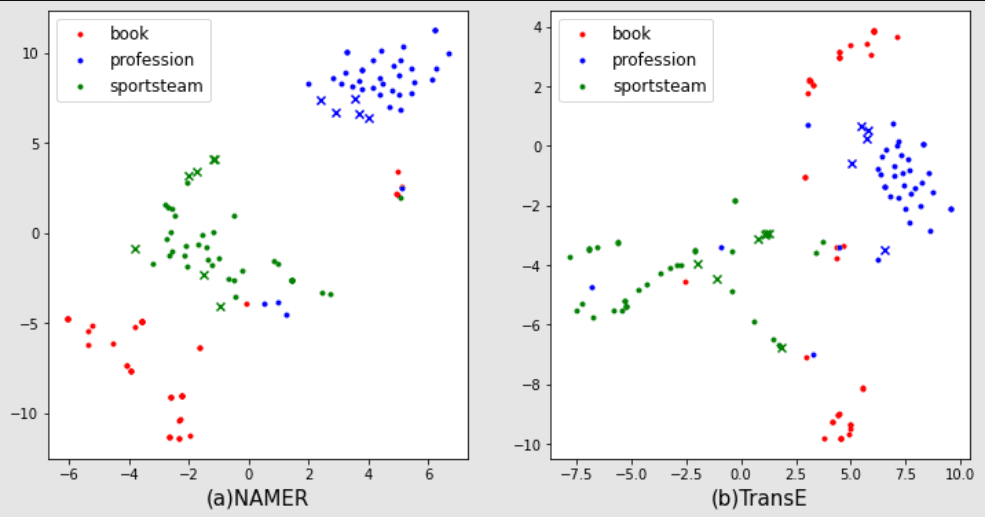
\includegraphics[width=0.75\textwidth]{4-1.png}
  \caption{实体嵌入可视化分析}
  \label{fig:4-1}
\end{figure}
图\ref{fig:4-1}中展示了本文提出的NAMER模型和去除元学习和本体嵌入的传统TransE模型在NELL-Ext数据集的测试集上实体嵌入的可视化。图中不同颜色展示了不同类型的实体,圆点代表未见的实体,叉号则代表了该类型下的已知实体。NAMER在实体获得初始化的向量表示后,通过两层GCN来学习邻域节点和相连关系的特征,使得同一类型的实体在表示空间上尽可能聚集在较紧密的邻域中。从可视化中也可以看出NAMER产生的嵌入分布与对应类型更加一致,在嵌入映射的距离上更近紧凑,而TransE-KGE产生的嵌入则混合了不同实体类型。NAMER将嵌入映射到了不同的聚类中,而TransE中不同实体类型的嵌入则混合在一起。此外,本文的模型在对未见的实体进行表示学习的过程中,采用聚合实体关系的特征来初始化实体向量,相邻关系的结构特征可以表现出实体的类型信息,因此模型可以将未见的实体的嵌入与同一类型的已知实体聚类。不同类型实体的聚类表明,NAMER能够用包含合理语义和信息性知识的嵌入来表示未见的实体。

\section{未见关系案例分析}
对于未见关系,本文同样选取了部分关系映射到了二维空间上进行可视化分析,如图\ref{fig:4-2}所示,其中圆点代表训练集中可见的关系,叉号代表测试集中的未见关系。
\begin{figure}[h]
  \centering
  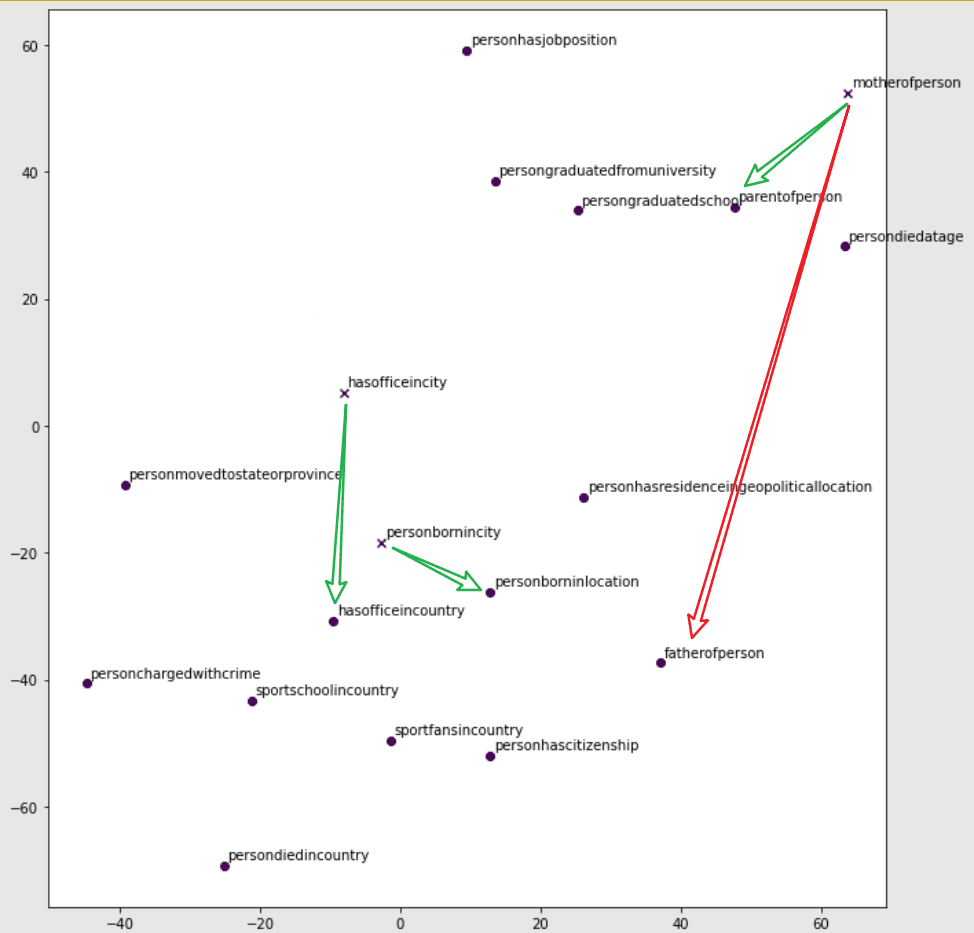
\includegraphics[width=0.7\textwidth]{4-2.png}
  \caption{实体嵌入可视化分析}
  \label{fig:4-2}
\end{figure}

本文模型通过采用关系位置图、根据关系的相对位置对关系局部的邻接关系进行建模学习到了关系的拓扑结构信息,同时引入本体信息作为语义补充,因此同一实体的具有相近语义的相邻关系在距离上应该表现为更加相近,从图上可以看出,对于未见关系has\_office\_in\_city贴近于具有类似语义的关系has\_office\_in\_coutry,未见关系person\_born\_in\_city更贴近于已知关系person\_born\_in\_location。而对于已知关系parent\_of\_person、father\_of\_person和未见关系mother\_of\_person,本文可知一个实体如果存在parent\_of\_person的关系那么该实体节点的邻接关系中只能存在其中一个father或者mother的关系,因此在图中本文可以观察到mother\_of\_person在距离上更接近于parent\_of\_person关系,而远离father\_of\_person关系。由此可见,本文模型通过在关系的位置图上联合本体语义信息有效的学习到了对应关系的语义关系,且其中相似的关系在向量空间中靠近,证明了本文提出的NAMER在嵌入未知关系方面的有效性。

\section{本章小结}
本章将本文提出的模型在测试数据集上NELL\_Ext和DB\_Ext上进行了链接预测任务的相关实验。与多个基准模型相比,本文提出的模型在任务得分上均有不同程度的提升,并通过对实验结果的分析验证了模型对于表示学习效果增强的有效性。同时通过对各个模型组件的消融实验发现明显的效果下降,证明了模型模块的重要性;最后对未见实体和未见关系的案例分析可知得到的嵌入表示符合模型原理设定,再次证明了该模型对未见组件表示上的突出能力。
\chapter{总结与展望}

\section{总结}
当下知识图谱技术的应用日益渗透到每个人的日常生活中,从搜索引擎到推荐系统,不断探索知识图谱知识的应用与补充是未来发展不可或缺的一个研究方向。但是出于数据隐私、成本等多方面的考量,大到公司多个图谱存储服务器,小到人们每日使用的移动终端,我们无法将所有分散知识图谱新添加的实体和关系完全覆盖。如何在源域知识图谱上训练,并且能够将表示学习能力泛化到应用于包含未见实体和关系的目标域知识图谱的研究是无可避免的需求。

面向跨域知识图谱的知识表示学习问题,本文采用了元学习的方法,在训练任务中模拟了跨域场景下的未见关系和未见实体,从而获得了模型处理未见组件的能力。元学习方法具有训练效率高的优点,可以在算力珍贵的时代大幅降低成本消耗。对于未见关系的表示能力学习,本文依据关系间的相对位置关系构建了一个以关系为结点的图,并通过预定义的元关系将其连接起来,以体现出关系的拓扑信息。此外,我们将本体信息嵌入作为关系语义信息的体现,再经过图卷积网络对关系节点进行拓扑信息和语义信息的联合学习,获得了对未见关系的表达。针对未见实体的表示能力学习,本文通过分析总结出相似类型实体在邻接结构上表现出高度相似性这一结论,并采用了实体的邻接关系特征聚合作为未见实体的初始化表示,避免了对未见实体周围节点的苛刻性要求。但聚合关系的表示仍然不足以支撑对实体特征的体现,为了能够充分利用到已知实体和关系的特征信息,我们使用CompGCN对实体和关系进行邻接信息的学习和更新,从而获得了各组件的嵌入。通过实验、基准模型比较和案例分析,本文证明了所提出模型的有效性。归纳起来,本文的工作主要包括:
\begin{enumerate}[label=\arabic*)]
  \item 为了充分捕捉到本体中实体和关系对应的语义信息,对本体三元组进行嵌入,学习到本体的向量表示。同时为了补充本体信息中的关系信息,构建了关系的位置元关系,补充了本体中的关系本体三元组。在本体三元组结构信息嵌入的基础上,基于描述文本进一步对本体嵌入加强。
  \item 在对跨域知识图谱的知识表示学习中引入了本体信息作为知识图谱的语义信息补充,通过对拓扑信息和语义信息的结合能够有效对未见实体和关系进行表示学习,同时采用复杂图卷积层对表示学习的效果进行加强,有效学习到了实体和关系的特征表示。模型总体采用元学习的任务设定对模型进行训练,在元学习的单任务中对跨域场景进行模拟,使得模型能够学习到处理未见实体和关系的能力,同时提高训练的效率,降低成本。
  \item 在两个知识图谱链接预测基准数据集的基础上构建满足跨域场景要求下的测试数据集,并与多个基准模型进行实验效果比较,通过对结果分析可知本文模型相比于其他基准模型均有不同程度的提升,证明了本文模型的有效性。
\end{enumerate}

\section{未来工作}
虽然本文在测试数据集上的效果相比于其他基准模型已经获得了明显的提升,但是在本文的整个研究过程中仍旧发现了当下模型在应用方面值得继续探究的几个研究方向:
\begin{enumerate}[label=\arabic*)]
  \item 本体嵌入的评分函数对模型效果的影响:在对本体的嵌入过程中,本文采用了目前传统KGE方法中效果最好的RotatE模型作为评分函数。但是从实验结果中我们可以发现对于DistMult和ComplEx评分函数的得分会比更简单的TransE更低,那么不同的本体嵌入方法可能对模型的效果会产生影响,是否本体嵌入评分函数和模型评分函数相对应会更获得更好的模型效果值得探究。
  \item 数据集本体信息的提取:本文模型研究本体信息对知识图谱表示学习的可用性,本体三元组是必不可少的一环。但当下的一些基准知识图谱有些并没有相应的本体三元组,如被广泛使用的FB15K-237数据集,因为其源数据集已经停止维护,本体类型信息也都比较杂乱无法使用。虽然本文在处理测试数据集时采用了对实例三元组类型信息补充了本体三元组中的关系信息,但面对一个数据集如何更充分获取到其本体信息仍旧是待解决的难题。
  \item 规则信息的引入:从DB\_Ext的基准模型测试信息可以看出基于规则提取的模型在未见的实体上也能够不错的表现效果,而且规则理论上可以同时作用于实体和关系,是对跨域知识图谱表示学习进行约束的良好设定。如何将规则信息融入到本文模型更好的学习到未见组件的表示也是未来工作的一个值得期待的方向。
\end{enumerate}
% \include{pages/chapter1}
% \include{pages/chapter2}
% \include{pages/chapter3}
% \include{pages/chapter4}
% \include{pages/chapter5}
% \include{pages/chapter6}
\end{document}
